% Elsevier submission build (CAS single-column class, els-cas-templates).
\documentclass[a4paper,fleqn]{cas-sc}
\usepackage[numbers,sort&compress]{natbib}
\usepackage{amsmath,amssymb,amsthm}
\usepackage{graphicx}
\graphicspath{{figures/}}
\usepackage{booktabs}
\usepackage{array}
\usepackage{microtype}
\usepackage{tikz}
\usetikzlibrary{positioning,arrows.meta,shapes.geometric,backgrounds,fit,calc}
\usepackage{float}
\usepackage{longtable}
% The class redefines the float mechanism at begin-document, which wipes
% the [H] placement that float.sty installs, so the two standard floats
% are restyled back after the class has finished.
\AtBeginDocument{\restylefloat{figure}\restylefloat{table}}
% Self-contained algorithm float and numbered pseudocode lines (no external
% algorithm packages; switch to algorithmicx at submission if preferred).
\floatstyle{ruled}
\newfloat{algorithm}{H}{loa}
\floatname{algorithm}{Algorithm}
\newcounter{algline}
\newenvironment{pseudolines}
  {\begin{list}{{\footnotesize\arabic{algline}:}}
     {\usecounter{algline}\setlength{\itemsep}{1pt}
      \setlength{\parsep}{0pt}\setlength{\topsep}{4pt}
      \setlength{\labelwidth}{1.4em}\setlength{\leftmargin}{2.2em}}}
  {\end{list}}
\newcommand{\kw}[1]{\textbf{#1}}
\newcommand{\algin}{\hspace*{1.4em}}
\newcommand{\algcomment}[1]{\hfill$\triangleright$~{\footnotesize #1}}
\emergencystretch=3em

\newtheorem{theorem}{Theorem}
\newtheorem{lemma}{Lemma}
\newtheorem{proposition}{Proposition}
\newtheorem{corollary}{Corollary}
\newtheorem{observation}{Observation}
\theoremstyle{definition}
\newtheorem{definition}{Definition}
\theoremstyle{remark}
\newtheorem{remark}{Remark}
\newtheorem{openproblem}{Open Problem}

\newcommand{\OPT}{\mathrm{OPT}}
\newcommand{\dist}{\mathrm{dist}}
\newcommand{\NP}{\textsf{NP}}
\newcommand{\Ppoly}{\textsf{P}}
\newcommand{\FPT}{\textsf{FPT}}
\newcommand{\XP}{\textsf{XP}}

\begin{document}
\let\WriteBookmarks\relax
\def\floatpagepagefraction{1}
\def\textpagefraction{.001}

\shorttitle{Parameterized complexity of the multiproduct two-stage
capacitated facility location problem}
\shortauthors{P.H. Gonz\'alez and R. Schneider}

\title[mode = title]{The Multiproduct Two-Stage Capacitated Facility
Location Problem: A Parameterized Complexity Analysis}

\author[1]{Pedro Henrique Gonz\'alez}
\cormark[1]
\ead{pegonzalez@cos.ufrj.br}

\author[1]{Rafael Schneider}
\ead{rschneider@cos.ufrj.br}

\affiliation[1]{organization={Federal University of Rio de Janeiro},
            city={Rio de Janeiro},
            country={Brazil}}

\cortext[1]{Corresponding author.}

\begin{abstract}
In the multiproduct two-stage capacitated facility location problem
(MP-TSCFLP), factories and depots open at fixed cost and route several
products to customers under per-product capacities and demands. Its
literature manages the difficulty with relaxations and hybrid
metaheuristics, and on the hundred-instance benchmark of Mauri and
coauthors no optimal value had, to our knowledge, ever been proven. We treat that
difficulty as a mathematical object. Parameterized analyses of
facility location cover uncapacitated single-stage variants, and we
give, to our knowledge, the first for the capacitated two-stage
multiproduct problem. Unless P equals NP, the four size parameters
obey a dichotomy in which the problem is fixed-parameter tractable
exactly when the parameter set contains both facility counts, through
a single algorithm exponential only in those two counts. One product
and one factory already force strong NP-hardness and logarithmic
set-cover inapproximability, while one customer and one product
isolate a numeric layer that separable first-stage costs render
pseudo-polynomial, strong hardness persisting outside the separable
class. In the number of opened facilities the problem is W[2]-hard,
and under the Exponential Time Hypothesis the direct enumeration is
optimal up to the constant in the exponent. Kernelization is delimited
from both sides, since no polynomial kernel exists in the facility
counts unless NP lies in coNP/poly, even under unary encodings,
whereas costs and total demands polynomially bounded in a slightly
larger parameter admit one. Roughly nine hundred thousand
computational checks validated every hardness gadget and the exact
codes, with no failure. The computational study closes three benchmark
instances to certified optimality for the first time, improving their
best-known values, and finds that a covering bound available before
any optimization tracks the tightness of the solver's root relaxation.
\end{abstract}

\begin{highlights}
\item First parameterized complexity analysis of the two-stage
multiproduct problem
\item The four size parameters obey a dichotomy around the two facility
counts
\item No polynomial kernel in the facility counts unless NP lies in
coNP/poly
\item W[2]-hardness in the opening count, with the XP enumeration
optimal under ETH
\item The covering bound tracks root relaxation tightness on the public
benchmark
\end{highlights}

\begin{keywords}
Facility Location \sep Supply Chain Design \sep Parameterized
Complexity \sep Fixed-Parameter Tractability \sep Kernelization Lower
Bounds \sep Branch-and-Bound
\MSC[2020] 90B80 \sep 68Q27 \sep 90C27
\end{keywords}

\maketitle

\section{Introduction}\label{sec:intro}

A manufacturer that supplies many markets rarely ships from the factory
gate to the customer in a single leg. Goods leave a small number of
production sites, pass through intermediate depots that consolidate and
break bulk, and only then reach the retailers. Deciding which factories
and which depots to operate, and how to route several products through
the two stages so that every demand is met at least total cost, is among
the oldest planning questions in distribution logistics
\citep{KloseDrexl2005,OrtizAstorquizaEtAl2018}, and it remains
a daily one wherever a supply chain is redesigned or a distribution
network is sized. The two layers interact from the start, because a depot
is worth opening only if some open factory can feed it and some customer
needs what it holds, so the fixed decisions and the transport decisions
cannot be taken apart, and it is this coupling that makes the problem more
than the sum of its two stages.

This interaction is captured by the multiproduct two-stage capacitated
facility location problem, which we abbreviate MP-TSCFLP. Several
products flow from candidate factories to candidate depots and on to
customers. Opening a factory or a depot costs a fixed charge, each unit
shipped on a stage carries a per-product transport cost, and every
factory and depot has a per-product capacity, while each customer has a
per-product demand that must be satisfied. Both stages are complete
bipartite, so any open factory may serve any depot and any open depot may
serve any customer. The uncapacitated single-product ancestor of the
model is the classical facility location problem, and the two-stage
capacitated multiproduct form was already observed to be \NP-hard by
\citet{PirkulJayaraman1998}. The benchmark and the solution methods we
build on are those of \citet{MauriEtAl2021}, who introduced the
hundred-instance benchmark and attacked it with two hybrid
metaheuristics, and of \citet{MoraisEtAl2022}, who later added local
branching to a genetic-algorithm hybrid for the same model.

Two facts recur in this literature, and both concern difficulty rather
than modelling. First, the instances resist exact solution. On the
hundred instances assembled by \citet{MauriEtAl2021} a commercial
mixed-integer solver solved none to proven optimality within a one-hour
budget per instance, which is why the authors turned to heuristics in the first place.
Second, this difficulty has no theoretical counterpart. Beyond the
inherited statement that the problem is \NP-hard
\citep{PirkulJayaraman1998}, no finer-grained account exists of \emph{where}
the hardness sits, which structural features drive it, or which of them could
be exploited to solve the problem faster.

This paper takes the empirical hardness as the phenomenon to be
explained. Facility location as such has a parameterized literature,
whose closest antecedent here is the parameterized view of
\citet{FellowsFernau2011}, a map of uncapacitated single-stage variants,
but no parameterized analysis covers the two-stage capacitated
multiproduct model, and we give what is, to our knowledge, the first. We
work throughout with the cardinality-constrained decision version, in which
a solution may open at most $k$ facilities, counting factories and depots
together, and $k$ is
the parameter that measures how lean a viable design is allowed to be.
Alongside $k$ we study the four size parameters of an instance, the numbers
$|I|$ of factories, $|J|$ of depots, $|K|$ of customers and $|L|$ of
products, both singly and in every combination. The guiding question is
which of these quantities, when held small, tames the exponential behaviour
of the problem, and which leave it intractable even when fixed. An
answer matters beyond taxonomy, because each tractable combination names
a regime in which exact solution scales, and each hard combination names
a feature whose cost no exact method avoids unless \Ppoly${}={}$\NP. The
analysis is a classification, so the algorithms it produces are devices for
locating the difficulty rather than candidates to beat a commercial solver,
and its practical residue is a covering bound that annotates an instance
before any optimisation is run.

Our findings fall into three groups, one locating the hardness along
the four dimensions, one drawing the tractability border together with
its preprocessing limits, and one certifying the map computationally and
confronting it with a solver. The hardness comes first because its
slices are the material from which the border is proved.

First, we locate the hardness. The problem collapses when all fixed
charges vanish and when a single factory faces a single depot
(Propositions~\ref{prop:fzero} and~\ref{prop:onebyone}), and hardness
begins one step above. With one product and one factory the problem is
already strongly \NP-hard, the depot-to-customer stage alone encoding a
covering problem, and no approximation beats the logarithmic Set Cover
threshold unless \Ppoly${}={}$\NP\ (Theorem~\ref{thm:cover},
Corollary~\ref{cor:coverinapprox}). Fixing any single size parameter to
a constant leaves the problem \NP-hard, which we prove through four
hard groups, each fixing two of the four dimensions to one. Behind the
groups sit four discrimination pairs, pairs in which one facility side
tells the members of another dimension apart through its cost matrix, a
notion Section~\ref{sec:complexity} fixes precisely, so hardness
survives every single restriction.

Second, we draw the tractability border. Parameterizing by any subset
$P$ of the four size parameters, the problem is fixed-parameter
tractable whenever $P$ contains both $|I|$ and $|J|$, through a single
$2^{|I|+|J|}\cdot\mathrm{poly}$ algorithm, and para-\NP-hard for every
other $P$, so under $\Ppoly\neq\NP$ the tractable subsets are exactly
those containing both (Theorem~\ref{thm:dichotomy}). MP-TSCFLP is
$\mathrm{W}[2]$-hard in the cardinality parameter $k$, already with one
product and one factory and already when only the depots are counted
(Theorem~\ref{thm:w2}), and under the Exponential Time Hypothesis the
naive $n^{k}$ enumeration is essentially optimal
(Theorem~\ref{thm:eth}). A separate numeric layer, our label for
hardness that persists after the combinatorial dimensions are
trivialised, governs the smallest instances. With a single customer and
a single product the problem is \NP-hard, separability of the
first-stage cost delimits a pseudo-polynomially solvable part, and
strong hardness persists outside the separable class, the general
boundary remaining open (Theorem~\ref{thm:numeric} and
Theorem~\ref{thm:separable}). On the preprocessing side, the problem
admits no polynomial kernel in $|I|+|J|$ unless
\NP${}\subseteq{}$coNP/poly (Theorem~\ref{thm:nokernel}), and over the
incidence representation we analyse the obstruction is numeric rather
than structural, for that incidence graph always has clique-width at
most two (Observation~\ref{obs:cliquewidth}). Several further positive
results, the pseudo-polynomial regimes and the
customer aggregation among them, are stated and classified but kept
outside the algorithmic core, since our aim is the map and not the
tuning of any one route through it.

Third, every construction behind the map is checked computationally.
The gadgets were validated by a shared battery of roughly
$9\times 10^{5}$ individual checks, none of which failed, and the enumeration algorithm agrees
with an independent brute-force solver across all $1{,}381$
comparisons. The computational study asks in what regime the
enumeration is practical and how it stands against Gurobi, the
mixed-integer baseline of Section~\ref{sec:experiments}. It then asks
whether the pruning threshold $k^{\ast}$ that our branch-and-bound
derives, available before any optimisation is run, tracks the
empirical difficulty of an instance, and through what mechanism it
does so. The protocol, instances and seeds are fixed in advance so
that every figure can be regenerated.

The remainder of this paper is organised as follows.
Section~\ref{sec:literature} places the model in the exact, heuristic and
parameterized literatures and closes with a positioning table.
Section~\ref{sec:prelim} fixes the model, proves the routing oracle,
that is the subroutine that, given a design, computes its optimal
routing cost, together with the
feasibility test and the monotonicity on which every later argument
rests, and maps the polynomial cases. Section~\ref{sec:complexity}
develops the four covering reductions, the numeric layer and the lower
bounds for the parameter $k$. Section~\ref{sec:algorithms} gives the
enumeration algorithm with its branch-and-bound, the dichotomy theorem
and the two sides of the kernelization question, and
Section~\ref{sec:experiments} reports the computational study built on
them. Section~\ref{sec:conclusion} states the two-layer synthesis and
five open problems.

\section{Related work}\label{sec:literature}

Two-stage capacitated facility location entered the operations research
literature as a distribution-planning model. General surveys of facility
location and of multi-level location are given by \citet{KloseDrexl2005}
and \citet{OrtizAstorquizaEtAl2018}.
\citet{PirkulJayaraman1998} formulated the multiproduct two-stage
capacitated version, observed its \NP-hardness and solved it by
Lagrangian relaxation, and this is the formulation that the later
benchmark work inherits. Exact and heuristic effort has continued on both
the single- and multi-stage variants. \citet{LitvinchevOzuna2012} derived
Lagrangian bounds for two-stage capacitated location, together with an
accompanying heuristic, and \citet{FernandesEtAl2014} proposed a simple
and effective genetic algorithm for the single-product two-stage problem
along with the large benchmark instance sets that the multiproduct
studies later reused. On the exact side, Benders decompositions tailored
to facility location are a mature computational line
\citep{FischettiLjubicSinnl2017}, and the disaggregated cuts of
Section~\ref{sec:certificates}, derived from the routing oracle of
Proposition~\ref{prop:oracle}, sit in that tradition. The benchmark this paper builds on is due
to \citet{MauriEtAl2021}, who assembled a hundred multiproduct instances
and, finding that a commercial mixed-integer solver closed none of them
within the imposed limits, proposed two hybrid metaheuristics, a
clustering search matheuristic that calls CPLEX on network-flow
subproblems and a biased random-key genetic algorithm with local search.
\citet{MoraisEtAl2022} then addressed the same multiproduct problem with
a hybrid biased random-key genetic algorithm that adds local branching,
extending a single-product hybrid from the same group. Across this line the model is treated as empirically hard, and
the hardness is managed rather than explained.

The complexity of facility location itself is well understood in the
uncapacitated single-product case, and it is where our covering arguments
originate. Without the metric assumption, uncapacitated facility location
contains Set Cover, so \citet{Hochbaum1982} obtained a greedy
$O(\log n)$ approximation, and the lower bounds recorded next show that no
better guarantee is possible in general unless $\Ppoly=\NP$.
The matching lower bounds are those of \citet{Feige1998} and, under the
weaker assumption \Ppoly${}\neq{}$\NP, of \citet{DinurSteurer2014},
which together pin the Set Cover threshold at $(1-\varepsilon)\ln n$.
These bounds transfer to the depot-to-customer stage of MP-TSCFLP and
account for its inapproximability. The classical hardness of the
underlying decision problems traces back to \citet{Karp1972}, and the
distinction between weak and strong \NP-hardness that organises our
numeric layer is that of \citet{GareyJohnson1979}.

Parameterized complexity has been brought to bear on optimisation and
covering problems for two decades, and the vocabulary and lower-bound
machinery we use are standard \citep{DowneyFellows2013,Cygan2015}. The
$\mathrm{W}[2]$-hardness of \textsc{Set Cover} parameterized by the
solution size is classical \citep{DowneyFellows2013}, the ETH-based lower
bounds we compose with are due to \citet{ChenHuangKanjXia2006}, and the
compression arguments in the kernelization section rely on
the number-reduction technique of \citet{FrankTardos1987}. The parameterized
view of location and network problems has grown quickly, though along axes
different from ours. The closest antecedent is the parameterized view of
facility location by \citet{FellowsFernau2011}, published in this
journal, which establishes W-hardness and \FPT\ results for
uncapacitated facility location variants under related parameters.
Capacities, a second stage and multiple products all lie outside its
scope, and that is the gap the present analysis fills.
Facility-location-flavoured clustering admits tight
fixed-parameter approximations in the number of centres
\citep{CohenAddadEtAl2019}. Under uniform capacities tight \FPT\
approximations in the number of centres remain available, and
constant-factor \FPT\ approximations with larger factors extend to the
general capacitated setting \citep{CohenAddadLi2019}. The survivable
network design problem is fixed-parameter tractable in its edge- and
element-connectivity forms while turning $\mathrm{W}[1]$-hard for vertex
connectivity \citep{FeldmannMukherjeevanLeeuwen2025}. Covering objectives
on structured graphs, tractable by treewidth alone in their nonnegative
form, in general require treewidth combined with maximum degree
\citep{FominRamamoorthi2022}. Each of the clustering, connectivity and
covering results turns on a metric, a connectivity
requirement or a graph width, whereas the hardness we isolate is arithmetic,
carried by capacities and demands, so their positive machinery does not
transfer to the representations analysed here, while richer
representations remain unanalysed rather than excluded. The contrast is sharpest on the
approximation side. What separates our covering core from the capacitated clustering results
is the absence of a metric. There the parameterized lower bounds have
recently caught up with the classical ones, since approximating
\textsc{Set Cover} parameterized by the solution size within any constant
factor is itself $\mathrm{W}[2]$-hard \citep{LinRenSunWang2023}. This suggests the same barrier for
MP-TSCFLP, a transfer we state as a conjecture among the open problems
of Section~\ref{sec:conclusion}. Closest in
spirit to the present analysis is the parameterized study of
minimum-weight solution subgraphs of and-or graphs by
\citet{DantasProttiSouza2013}, where a cheapest subnetwork must respect
local dependency semantics and zero-weight arcs are exactly what turns a
fixed-parameter tractable problem $\mathrm{W}[2]$-hard. Zero fixed charges play a
comparable role in our constructions, which require either large numbers,
many products or positive charges to produce hardness.

Table~\ref{tab:positioning} closes the section by placing this paper
against the works discussed above, one line per selected work and one
column per feature, with a mark recording only what the corresponding
paragraph of this section states. The last line of the table records a
combination of features that no previous line fills, a parameterized
analysis of the two-stage capacitated multiproduct model.

\begin{table}[H]
\footnotesize
\centering
\caption{Positioning against the related work of this section. A check
mark means the feature is treated in the cited work as described above.
The circle marks bounds or partial guarantees claimed without an
exactness or completeness proof. Blank means not
treated.}
\label{tab:positioning}
\resizebox{\textwidth}{!}{%
\begin{tabular}{lcccccc}
\toprule
 & two-stage & multi- & capa- & exact or & heuris- & parameterized \\
 & location & product & cities & lower bounds & tics & analysis \\
\midrule
\citet{PirkulJayaraman1998} & \checkmark & \checkmark & \checkmark &
$\circ$ & \checkmark & \\
\citet{LitvinchevOzuna2012} & \checkmark & & \checkmark & $\circ$ &
\checkmark & \\
\citet{FernandesEtAl2014} & \checkmark & & \checkmark &
 & \checkmark & \\
\citet{MauriEtAl2021} & \checkmark & \checkmark & \checkmark & &
\checkmark & \\
\citet{MoraisEtAl2022} & \checkmark & \checkmark & \checkmark & &
\checkmark & \\
\citet{DantasProttiSouza2013} & & & & \checkmark & & \checkmark \\
\citet{CohenAddadLi2019} & & & \checkmark & $\circ$ & &
\checkmark \\
\citet{FeldmannMukherjeevanLeeuwen2025} & & & & \checkmark & &
\checkmark \\
This paper & \checkmark & \checkmark & \checkmark & \checkmark & &
\checkmark \\
\bottomrule
\end{tabular}}
\end{table}

\section{Problem definition and structural properties}\label{sec:prelim}

This section fixes the model, records its decision versions and the
parameterized objects we study, and collects the structural facts that
the later sections use as tools. The facts are elementary but used
throughout the subsequent proofs, so we prove them in full, with the
three longest proofs collected in Appendix~\ref{app:proofs}. Each is additionally checked
computationally, over the bounded instance families recorded in the
accompanying software archive.

An instance of MP-TSCFLP is given by four finite sets, the factories
$I$, the depots $J$, the customers $K$ and the products $L$, together
with nonnegative integer data. Opening factory $i$ costs $f_i$ and
opening depot $j$ costs $g_j$. Shipping one unit of product $l$ from
factory $i$ to depot $j$ costs $c_{ijl}$, and shipping it from depot $j$
to customer $k$ costs $d_{jkl}$. Factory $i$ can supply $b_{il}$ units of
product $l$ and depot $j$ can hold $p_{jl}$, while customer $k$ demands
$q_{kl}$. Both stages are complete bipartite, so no arc is forbidden a
priori. A solution opens a set of factories and depots, encoded by
$y\in\{0,1\}^{|I|}$ and $z\in\{0,1\}^{|J|}$, and routes the products through
nonnegative flows $x_{ijl}$ on the first stage and $w_{jkl}$ on the
second. We write $D_l=\sum_{k\in K}q_{kl}$ for the total demand of
product $l$ and $n=|I|+|J|$ for the number of candidate facilities.
Following \citet{MauriEtAl2021,PirkulJayaraman1998}, the problem
minimizes total cost,
\begin{align}
\min\;&\sum_{i\in I}f_iy_i+\sum_{j\in J}g_jz_j
      +\sum_{i,j,l}c_{ijl}\,x_{ijl}+\sum_{j,k,l}d_{jkl}\,w_{jkl}
\label{eq:obj}\\
\text{s.t.}\;
&\textstyle\sum_{j\in J}w_{jkl}\ge q_{kl}
   &&\forall k\in K,\ l\in L,\label{eq:C1}\\
&\textstyle\sum_{i\in I}x_{ijl}\ge\sum_{k\in K}w_{jkl}
   &&\forall j\in J,\ l\in L,\label{eq:C2}\\
&\textstyle\sum_{j\in J}x_{ijl}\le b_{il}\,y_i
   &&\forall i\in I,\ l\in L,\label{eq:C3}\\
&\textstyle\sum_{k\in K}w_{jkl}\le p_{jl}\,z_j
   &&\forall j\in J,\ l\in L,\label{eq:C4}\\
&y_i,z_j\in\{0,1\},\quad x_{ijl},w_{jkl}\ge 0.\label{eq:dom}
\end{align}
Constraint~\eqref{eq:C1} serves each demand, \eqref{eq:C2} balances flow
through a depot, and \eqref{eq:C3} and~\eqref{eq:C4} cap the throughput of
a factory and a depot by its capacity while forcing the facility open
before any flow may use it. At $y_i=0$ the right-hand side
of~\eqref{eq:C3} vanishes and nonnegativity forces $x_{ijl}=0$ for every
$j$ and $l$, and \eqref{eq:C4} acts on the $w_{jkl}$ in the same way at
$z_j=0$. Capacities and demands are per product and
never couple two products, a feature the analysis exploits throughout.
Figure~\ref{fig:network} shows the two-stage network and the decisions a
solution fixes.

% Requires: \usetikzlibrary{positioning,arrows.meta,shapes.geometric}
\begin{figure}[H]
  \centering
  \resizebox{0.86\textwidth}{!}{%
  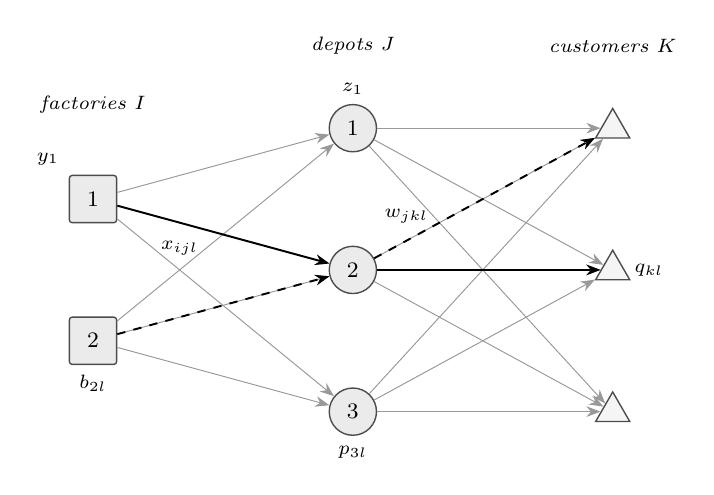
\begin{tikzpicture}[
      >={Stealth[length=1.8mm]},
      thin,
      every node/.style={font=\footnotesize},
      fac/.style={draw=black!70,line width=0.5pt,fill=black!8,rounded corners=1pt,minimum size=6mm,inner sep=1pt},
      dep/.style={draw=black!70,line width=0.5pt,circle,fill=black!8,minimum size=6mm,inner sep=0pt},
      cus/.style={draw=black!70,line width=0.5pt,regular polygon,regular polygon sides=3,fill=black!4,minimum size=5mm,inner sep=0pt},
      lite/.style={draw=black!40,line width=0.35pt,->},
      p1/.style={draw=black,line width=0.7pt,->},
      p2/.style={draw=black,line width=0.7pt,dashed,->}
    ]
    % factories I
    \node[fac] (i1) at (0,2.1) {$1$};
    \node[fac] (i2) at (0,0.3) {$2$};
    % depots J
    \node[dep] (j1) at (3.3,3.0) {$1$};
    \node[dep] (j2) at (3.3,1.2) {$2$};
    \node[dep] (j3) at (3.3,-0.6) {$3$};
    % customers K
    \node[cus] (k1) at (6.6,3.0) {};
    \node[cus] (k2) at (6.6,1.2) {};
    \node[cus] (k3) at (6.6,-0.6) {};
    % layer captions
    \node[font=\scriptsize\itshape] at (0,3.3) {factories $I$};
    \node[font=\scriptsize\itshape] at (3.3,4.05) {depots $J$};
    \node[font=\scriptsize\itshape] at (6.6,4.05) {customers $K$};
    % stage-1 complete bipartite (light)
    \foreach \a in {i1,i2}{\foreach \b in {j1,j2,j3}{\draw[lite] (\a) -- (\b);}}
    % stage-2 complete bipartite (light)
    \foreach \a in {j1,j2,j3}{\foreach \b in {k1,k2,k3}{\draw[lite] (\a) -- (\b);}}
    % highlighted multiproduct arcs (two products)
    \draw[p1] (i1) -- (j2);
    \draw[p2] (i2) -- (j2);
    \draw[p1] (j2) -- (k2);
    \draw[p2] (j2) -- (k1);
    % annotations, each placed in a stroke-free pocket
    \node[anchor=south east,font=\scriptsize] at (i1.north west) {$y_1$};
    \node[anchor=north,font=\scriptsize] at (i2.south) {$b_{2l}$};
    \node[anchor=south,font=\scriptsize] at (j1.north) {$z_1$};
    \node[anchor=north,font=\scriptsize] at (j3.south) {$p_{3l}$};
    \node[font=\scriptsize] at (1.1,1.48) {$x_{ijl}$};
    \node[font=\scriptsize] at (3.98,1.88) {$w_{jkl}$};
    \node[anchor=west,font=\scriptsize] at (k2.east) {$q_{kl}$};
  \end{tikzpicture}%
  }
  \caption{The MP-TSCFLP network of
  model~\eqref{eq:obj}--\eqref{eq:dom}. A designer opens factories
  ($y_i$) and depots ($z_j$), after which each product flows across two
  capacitated stages, from factories through depots to customers, along
  stage-1 arcs carrying $x_{ijl}$ and stage-2 arcs carrying $w_{jkl}$.
  Factory capacities $b_{il}$ and depot capacities $p_{jl}$ bound the
  flow, which must meet every customer demand $q_{kl}$. The heavy solid
  arcs trace product $l=1$ and the heavy dashed arcs product $l=2$, so
  the two line styles convey the multiproduct structure, while the light
  arcs show that both stages are complete. The coupling of the two stages
  through the depots is the interaction that the reductions of
  Section~\ref{sec:complexity} turn into hardness.}
  \label{fig:network}
\end{figure}


A tiny instance already shows the interaction that drives the hardness.
Take one product and one factory of ample capacity, two depots and three
customers, with unit second-stage cost $d_{jk}$ equal to $0$ when depot
$j$ can reach customer $k$ cheaply and to $1$ otherwise, the product
index suppressed as there is a single product. Choosing which
depots to open so that every customer is served through a zero-cost arc
is exactly a set-cover decision, and no amount of first-stage freedom
removes it, because the single factory feeds whichever depots are open.
A core of the problem's combinatorial difficulty is thus already present
in the second stage, and the reductions of Section~\ref{sec:complexity}
grow from this observation.

The optimization problem has two decision versions. In the first only the
budget is bounded, and in the second the number of opened facilities is
bounded as well, which is the version we parameterize.

\begin{definition}[$\mathrm{MP\text{-}TSCFLP}(B)$]\label{def:B}
Given an MP-TSCFLP instance and an integer $B\ge 0$, decide whether some
feasible solution has total cost at most $B$.
\end{definition}

\begin{definition}[$\mathrm{MP\text{-}TSCFLP}(B,k)$]\label{def:Bk}
Given an MP-TSCFLP instance and integers $B\ge 0$ and $k\ge 0$, decide
whether some feasible solution has total cost at most $B$ and opens at
most $k$ facilities, that is $\sum_{i}y_i+\sum_{j}z_j\le k$. The
parameter is $k$.
\end{definition}

A tempting alternative would parameterize by the number of facilities
open in an optimal solution. Solution-dependent parameters are studied
in other settings, but this one is not well defined here, because the
optimum is not unique.
When a closed facility carries zero fixed charge, opening it yields
another optimum, since by Proposition~\ref{prop:mono} below the total
cost cannot rise and optimality of the original solution means it cannot
fall. On such instances the count can therefore
vary by up to $n$ depending on which optimum one names, so we do not
adopt it. Turning the count into an explicit
budget repairs the defect, and setting $k=n$ recovers
Definition~\ref{def:B}, so nothing is lost.

We phrase the complexity statements in the standard parameterized
vocabulary, which we recall briefly following
\citet{DowneyFellows2013} and \citet{Cygan2015}. A parameterized problem
is fixed-parameter tractable, in the class \FPT, when it is solvable in
time $h(p)\cdot\mathrm{poly}(N)$ for a computable function $h$ of the
parameter $p$, with $N$ the instance size, and it lies in \XP\ when the
polynomial degree may depend on $p$. A problem that is \NP-hard already at
a fixed value of $p$ is para-\NP-hard and, unless $\Ppoly=\NP$, admits
neither an \FPT\ nor an \XP\ algorithm. We call a parameterization
strongly para-\NP-hard when some fixed slice is strongly \NP-hard, so
that the exclusion survives a unary encoding.\footnote{The term is our
coinage for the combination, para-\NP-hardness witnessed by a strongly
\NP-hard slice, and we are not aware of an established name.} Hardness within the W
hierarchy is transferred by \FPT\ reductions. An \FPT\ reduction maps an
instance of one parameterized problem to an equivalent instance of
another in \FPT\ time, with the parameter of the image bounded by a
computable function of the source parameter
\citep{DowneyFellows2013,Cygan2015}. A parameterized problem is
W[2]-hard when some W[2]-complete problem, \textsc{Set Cover}
parameterized by the cover size for instance, admits an \FPT\ reduction
to it, and a W[2]-hard problem is fixed-parameter tractable only if
every problem in W[2] is, which is considered implausible. A kernel is a
polynomial-time self-reduction that maps an instance to an equivalent
instance of the same problem whose size is bounded by a computable
function of $p$ alone, and a polynomial kernel is one whose size bound is
polynomial. More generally, a polynomial compression is a polynomial-time
reduction that maps an instance of a parameterized problem to an
equivalent instance of some fixed problem, not necessarily the same one,
whose size is bounded by a polynomial of the parameter alone. A
polynomial kernel is thus the special case of a polynomial compression in
which the target problem is the problem itself.

The first structural fact isolates the routing subproblem. Once the open
facilities are fixed the remaining decisions are pure transport, and
because capacities and costs never couple products the transport splits
into one independent flow per product. Each such flow is an ordinary
minimum-cost flow on a layered network, which both makes the residual
value computable in strongly polynomial time and, by total unimodularity,
forces it to be an integer. A routing for the fixed design $(y,z)$ is a
pair of nonnegative flow vectors $(x,w)$ satisfying
\eqref{eq:C1}--\eqref{eq:C4} with $(y,z)$ held fixed, and its block $l$ is
the slice of $(x,w)$ formed by the variables of product $l$. We write
$v(y,z)$ for the least total cost of a routing for the design, a minimum
that Proposition~\ref{prop:oracle} shows to be attained whenever a routing
exists, with the convention $v(y,z)=+\infty$ when no routing exists, that
is when the design is infeasible.

\paragraph{The layered network} For a fixed design $(y,z)$ and a product
$l$, build the network $N_l(y,z)$ with a source $S$, a sink $T$, one node
per open factory ($y_i=1$), one node per customer, and, for each open
depot ($z_j=1$), a split pair $j_{\mathrm{in}}\!\to\! j_{\mathrm{out}}$.
The arcs are as follows. From the source, each $S\!\to\! i$ has capacity
$b_{il}$ and cost $0$. Each $i\!\to\! j_{\mathrm{in}}$ has infinite
capacity and cost $c_{ijl}$, the split arc
$j_{\mathrm{in}}\!\to\! j_{\mathrm{out}}$ has capacity $p_{jl}$ and cost
$0$, each $j_{\mathrm{out}}\!\to\! k$ has infinite capacity and cost
$d_{jkl}$, and each $k\!\to\! T$ has capacity $q_{kl}$ and cost $0$. A
closed facility contributes no node, so its flow is forced to $0$, in
accordance with the vanishing right-hand sides of \eqref{eq:C3}
and~\eqref{eq:C4} noted after the model. An open depot caps its throughput at $p_{jl}$
through the split arc, which is~\eqref{eq:C4} at $z_j=1$, and the
source-arc capacity $b_{il}$ of an open factory is~\eqref{eq:C3} at
$y_i=1$. Every $S$--$T$ path has the form
$S\!\to\! i\!\to\! j_{\mathrm{in}}\!\to\! j_{\mathrm{out}}\!\to\! k\!\to\!
T$, because every arc leads from one layer of nodes to the next and no
arc skips a layer or returns to an earlier one.
Figure~\ref{fig:oraclenet} draws $N_l(y,z)$ for a small design and
labels each arc family with its capacity, its cost and the model
variable it carries.

% Requires: \usetikzlibrary{positioning,arrows.meta,shapes.geometric}
\begin{figure}[H]
  \centering
  \resizebox{0.96\textwidth}{!}{%
  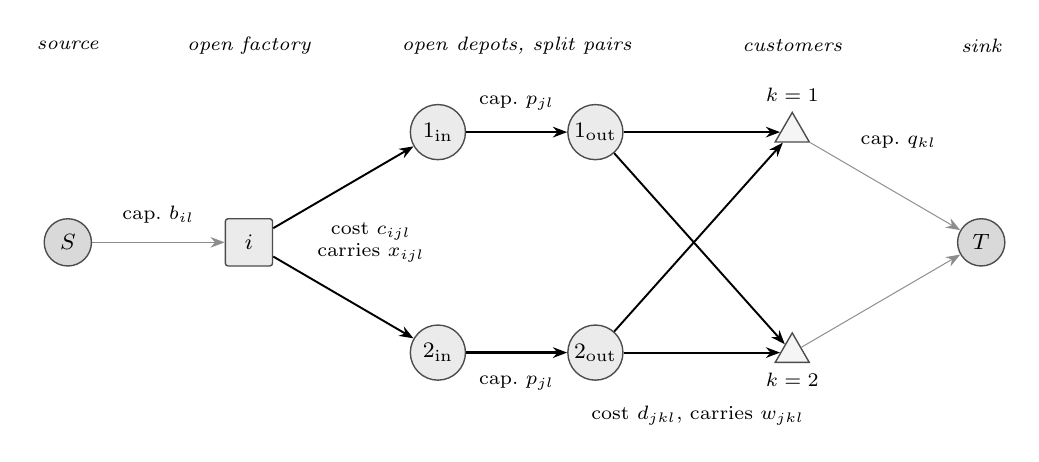
\begin{tikzpicture}[
      >={Stealth[length=1.8mm]},
      thin,
      every node/.style={font=\footnotesize},
      term/.style={draw=black!70,line width=0.5pt,circle,fill=black!15,minimum size=6mm,inner sep=1pt},
      fac/.style={draw=black!70,line width=0.5pt,fill=black!8,rounded corners=1pt,minimum size=6mm,inner sep=1pt},
      dep/.style={draw=black!70,line width=0.5pt,circle,fill=black!8,minimum size=7mm,inner sep=0pt},
      cus/.style={draw=black!70,line width=0.5pt,regular polygon,regular polygon sides=3,fill=black!4,minimum size=5mm,inner sep=0pt},
      capr/.style={draw=black!45,line width=0.35pt,->},
      cost/.style={draw=black,line width=0.7pt,->},
      splt/.style={draw=black,line width=0.9pt,->}
    ]
    % source and sink
    \node[term] (S) at (0,0.9) {$S$};
    \node[term] (T) at (11.6,0.9) {$T$};
    % open factory
    \node[fac] (i1) at (2.3,0.9) {$i$};
    % split pairs of the two open depots
    \node[dep] (j1in) at (4.7,2.3) {$1_{\mathrm{in}}$};
    \node[dep] (j1out) at (6.7,2.3) {$1_{\mathrm{out}}$};
    \node[dep] (j2in) at (4.7,-0.5) {$2_{\mathrm{in}}$};
    \node[dep] (j2out) at (6.7,-0.5) {$2_{\mathrm{out}}$};
    % customers
    \node[cus] (k1) at (9.2,2.3) {};
    \node[cus] (k2) at (9.2,-0.5) {};
    \node[font=\scriptsize,anchor=south] at (k1.north) {$k=1$};
    \node[font=\scriptsize,anchor=north] at (k2.south) {$k=2$};
    % layer captions
    \node[font=\scriptsize\itshape] at (0,3.4) {source};
    \node[font=\scriptsize\itshape] at (2.3,3.4) {open factory};
    \node[font=\scriptsize\itshape] at (5.7,3.4) {open depots, split pairs};
    \node[font=\scriptsize\itshape] at (9.2,3.4) {customers};
    \node[font=\scriptsize\itshape] at (11.6,3.4) {sink};
    % source arc: capacity b_il, cost 0
    \draw[capr] (S) -- (i1);
    \node[font=\scriptsize,anchor=south] at (1.15,1.02) {cap.\ $b_{il}$};
    % first-stage arcs: cost c_ijl, carry x_ijl; label inside the wedge
    \draw[cost] (i1) -- (j1in);
    \draw[cost] (i1) -- (j2in);
    \node[font=\scriptsize,align=center] at (3.85,0.9)
      {cost $c_{ijl}$\\ carries $x_{ijl}$};
    % split arcs: capacity p_jl, cost 0
    \draw[splt] (j1in) -- (j1out);
    \draw[splt] (j2in) -- (j2out);
    \node[font=\scriptsize,anchor=south] at (5.7,2.45) {cap.\ $p_{jl}$};
    \node[font=\scriptsize,anchor=north] at (5.7,-0.68) {cap.\ $p_{jl}$};
    % second-stage arcs: cost d_jkl, carry w_jkl; label below the network
    \draw[cost] (j1out) -- (k1);
    \draw[cost] (j1out) -- (k2);
    \draw[cost] (j2out) -- (k1);
    \draw[cost] (j2out) -- (k2);
    \node[font=\scriptsize,anchor=north] at (8.0,-1.05)
      {cost $d_{jkl}$, carries $w_{jkl}$};
    % demand arcs: capacity q_kl, cost 0; label above the upper arc
    \draw[capr] (k1) -- (T);
    \draw[capr] (k2) -- (T);
    \node[font=\scriptsize,anchor=south] at (10.55,1.97) {cap.\ $q_{kl}$};
  \end{tikzpicture}%
  }
  \caption{The layered network $N_l(y,z)$ of
  Proposition~\ref{prop:oracle} for one product $l$, drawn for a design
  with one open factory, two open depots and two customers. Source arcs
  $S\to i$ have capacity $b_{il}$ and cost $0$, each arc
  $i\to j_{\mathrm{in}}$ costs $c_{ijl}$ and carries the model variable
  $x_{ijl}$, each split arc $j_{\mathrm{in}}\to j_{\mathrm{out}}$ has
  capacity $p_{jl}$ and cost $0$, each arc $j_{\mathrm{out}}\to k$ costs
  $d_{jkl}$ and carries $w_{jkl}$, and each demand arc $k\to T$ has
  capacity $q_{kl}$ and cost $0$. This correspondence between the arc
  families and the model variables is the content of the proposition's
  proof.}
  \label{fig:oraclenet}
\end{figure}


\begin{proposition}[routing oracle]\label{prop:oracle}
Fix $(y,z)\in\{0,1\}^{|I|}\times\{0,1\}^{|J|}$. The residual routing problem
separates over products, and for each product $l$ its optimal cost equals
the minimum cost $\mu_l$ of an $S$--$T$ flow of value $D_l$ in the layered
network $N_l(y,z)$ defined above, with $\mu_l=+\infty$ when no such flow
exists. The finite $\mu_l$ are attained by integral flows and are
nonnegative integers, and $v(y,z)=\sum_l\mu_l$. Hence $v(y,z)$ is
computable in strongly polynomial time by $|L|$ minimum-cost flow
computations \citep{Orlin1993}.
\end{proposition}
The proof identifies each per-product block with a minimum-cost flow of
value $D_l$ in the layered network $N_l(y,z)$, matching routings and
flows in both directions at equal cost after a trimming step that
tightens \eqref{eq:C1} and~\eqref{eq:C2}. Total unimodularity of the
node--arc incidence matrix makes every finite block optimum an integer
attained by an integral flow. Summing the blocks delivers the identity
$v(y,z)=\sum_l\mu_l$ used throughout the paper. The full proof is in
Appendix~\ref{app:proofs}.

Whether a fixed design can serve the demand at all is settled without
solving any flow, by an aggregate test on each product. The completeness
of the two stages is what makes the test exact, since any open factory
reaches any open depot and any open depot reaches any customer, so only
the totals matter.

\begin{proposition}[feasibility]\label{prop:feas}
A design $(y,z)$ is feasible if and only if, for every product $l$,
\begin{equation}
\textstyle\sum_{i\in I}b_{il}\,y_i\ \ge\ D_l
\quad\text{(F1)}\qquad\text{and}\qquad
\sum_{j\in J}p_{jl}\,z_j\ \ge\ D_l\quad\text{(F2)}.
\label{eq:feas}
\end{equation}
The test runs in $O((n+|K|)\,|L|)$ time, of which $O(|K|\,|L|)$ computes
the totals $D_l$.
\end{proposition}
Necessity follows by aggregating the four constraint groups per
product, which bounds the served demand by the total open capacity of
each of the two layers, a two-cut argument. Sufficiency exhibits an
explicit flow of value $D_l$ in $N_l(y,z)$ through northwest-corner
transport constructions on the two complete stages, so the aggregate
test (F1) and (F2) is exact. The full proof is in Appendix~\ref{app:proofs}.

The characterization rests on the completeness of the two stages in an
essential way, and the following counterexample shows that
the dependence is real rather than an artefact of the proof.

\begin{remark}[completeness is essential]\label{rem:sparse}
The aggregate test fails once an arc may be forbidden, a forbidden arc
being modelled by deleting its flow variable. Take one product, two
factories, two depots and one customer, and open all four facilities.
Since there is a single product and a single customer we drop those
indices and write $b_i$, $p_j$ and $D$ for the capacities and the
demand, with $b_1=b_2=1$, $p_1=p_2=1$ and $D=2$, so (F1) and (F2) both
read $2\ge 2$ and hold. Suppose the first stage is sparse and both
factories may ship only to depot $1$. Depot $2$ then receives nothing,
so \eqref{eq:C2} forces it to forward nothing, while depot $1$ forwards
at most one unit by~\eqref{eq:C4}. The customer therefore receives at
most one unit, which violates \eqref{eq:C1} against the demand of two,
so no routing exists although both tests pass. The per-product totals no
longer determine feasibility, which is why the characterization is
stated only for the complete model.
\end{remark}

Opening more facilities preserves feasibility and never raises the
routing cost, only the fixed charge. This monotonicity underlies both the polynomial
cases below and the admissible bound used by the enumeration algorithm.

\begin{proposition}[monotonicity]\label{prop:mono}
If $(y,z)\le(y',z')$ componentwise then feasibility of $(y,z)$ implies
feasibility of $(y',z')$, and $v(y',z')\le v(y,z)$ always, with the
convention $v=+\infty$ on infeasible designs. In particular the all-open
design attains the least routing value among all feasible designs.
\end{proposition}
The feasibility part holds because the left-hand sides of (F1) and
(F2) are nondecreasing in the design. For the value part, $N_l(y,z)$ is
a subnetwork of $N_l(y',z')$, so every value-$D_l$ flow of the smaller
network is one of the larger network at the same cost and no block
optimum increases. Enlarging a design therefore preserves feasibility
and never raises the routing value, which is the form in which later
sections use the proposition. The full proof is in Appendix~\ref{app:proofs}.

Two regimes collapse to polynomial-time problems. When all fixed charges
vanish the fixed cost drops out and monotonicity makes opening everything
optimal, and when a single factory faces a single depot the routing is
forced and the optimum has a closed form.

\begin{proposition}[polynomial cases]\label{prop:fzero}
If $f\equiv 0$ and $g\equiv 0$, then MP-TSCFLP is solvable in strongly
polynomial time, its instance is feasible exactly when
$\sum_i b_{il}\ge D_l$ and $\sum_j p_{jl}\ge D_l$ for every $l$, and its
optimum is the all-open routing value $v(\mathbf 1,\mathbf 1)$.
\end{proposition}
\begin{proof}
With no fixed charge the cost of a design is its routing
value alone. By Proposition~\ref{prop:mono} the all-open design attains
the least routing value among feasible designs, and by
Proposition~\ref{prop:feas} it is feasible precisely under the displayed
conditions, which are (F1) and (F2) at $(y,z)=(\mathbf 1,\mathbf 1)$. If
they fail, no design at all is feasible, for every design lies
componentwise below $(\mathbf 1,\mathbf 1)$, so its feasibility would
imply that of the all-open design by the feasibility part of
Proposition~\ref{prop:mono}. In the feasible case the all-open design is
itself a solution of cost $v(\mathbf 1,\mathbf 1)$, and no feasible
design costs less, so the optimum equals $v(\mathbf 1,\mathbf 1)$,
computed in strongly polynomial time by Proposition~\ref{prop:oracle}.
\end{proof}

The second polynomial regime fixes one facility on each side. There the
design is forced and the optimum admits a closed form.

\begin{proposition}[single factory and depot]\label{prop:onebyone}
If $|I|=|J|=1$, then MP-TSCFLP is solvable in $O(|K|\,|L|)$ time after
reading the input, and feasibility reduces to $b_{1l}\ge D_l$ and
$p_{1l}\ge D_l$ for every $l$. When the instance is feasible and some
demand is positive the optimum equals
$f_1+g_1+\sum_{l}\bigl(c_{11l}D_l+\sum_k d_{1kl}q_{kl}\bigr)$, and when all
demand is zero the optimum is $0$, attained by opening nothing.
\end{proposition}
\begin{proof}
Feasibility forces the design, and nonnegativity of the costs then
makes the cheapest routing explicit. By
Proposition~\ref{prop:feas}, a design $(y_1,z_1)$
is feasible if and only if $b_{1l}y_1\ge D_l$ and $p_{1l}z_1\ge D_l$ for
every $l$, which is what (F1) and (F2) read with one facility per side.
If all demand is zero, these conditions hold for every design and the
stated condition holds because every $D_l$ equals $0$. In that case the
empty design is feasible, since (F1) and (F2) read $0\ge 0$ and the
all-zero routing satisfies \eqref{eq:C1}--\eqref{eq:C4}, and its cost $0$
is optimal by nonnegativity of the costs. Otherwise some $D_l>0$, and
any feasible design has $y_1=z_1=1$, since $y_1=0$ or $z_1=0$ would make
(F1) or (F2) read $0\ge D_l>0$. For such a design the conditions become
$b_{1l}\ge D_l$ and $p_{1l}\ge D_l$, so the instance is feasible exactly
under the stated condition, and feasibility forces the fixed charge to be
exactly $f_1+g_1$. The only remaining variables are $x_{11l}$ and
$w_{1kl}$. Feasibility needs $w_{1kl}\ge q_{kl}$ by~\eqref{eq:C1} and
$x_{11l}\ge\sum_k w_{1kl}\ge D_l$ by~\eqref{eq:C2}, and since all costs
are nonnegative the cheapest choice is $w_{1kl}=q_{kl}$ and
$x_{11l}=D_l$, of cost $\sum_k d_{1kl}q_{kl}$ on the second stage and
$c_{11l}D_l$ on the first. This choice is itself feasible, since
\eqref{eq:C3} reads $x_{11l}=D_l\le b_{1l}$ and \eqref{eq:C4} reads
$\sum_k w_{1kl}=D_l\le p_{1l}$, both guaranteed by the feasibility
condition, while \eqref{eq:C1} and~\eqref{eq:C2} hold with equality. No
feasible routing costs less, since its variables dominate this choice
componentwise by the bounds just derived and every cost coefficient is
nonnegative. Summing over $l$ and adding $f_1+g_1$ gives the closed
form, evaluated in $O(|K||L|)$ time.
\end{proof}

Finally, the cardinality version sits in \XP\ by brute force over the
opening pattern, a bound the algorithms of
Section~\ref{sec:algorithms} later refine and, under the Exponential
Time Hypothesis, match up to the constant in the exponent.

\begin{observation}[membership in \XP]\label{obs:xp}
$\mathrm{MP\text{-}TSCFLP}(B,k)$ is decidable in time
$n^{k+O(1)}\cdot\mathrm{poly}(N)$, with $N$ the instance size. When $n=0$ the empty
design is the only design, one application of
Propositions~\ref{prop:oracle} and~\ref{prop:feas} to it decides the
instance in polynomial time, and the counting below is not needed, so
assume $n\ge 1$. One may further normalize $k\le n$, since no design
opens more than $n$ facilities. Enumerating every set
$S\subseteq I\cup J$ of at most $k$ facilities then decides the
instance. Each $S$ is identified with the design $(y,z)$ whose
indicators it defines, so that $v(S)$ denotes $v(y,z)$, feasibility of
$S$ is tested by Proposition~\ref{prop:feas}, and for feasible $S$ the
total cost
$\sum_{i\in S\cap I}f_i+\sum_{j\in S\cap J}g_j+v(S)$ is evaluated with
$v(S)$ from
Proposition~\ref{prop:oracle}. The answer is \textsc{yes} if and only if
some such cost is at most $B$, since by the definition of $v$ the
cheapest solution whose opening pattern is $S$ costs exactly this
amount, and every solution opening at most $k$ facilities has its
pattern among the enumerated sets. The number of sets is
$\sum_{r=0}^{k}\binom{n}{r}\le\sum_{r=0}^{k}n^{r}\le(k+1)\,n^{k}$, using
$\binom{n}{r}\le n^{r}\le n^{k}$ for $r\le k$ and $n\ge 1$. Each set is
processed in polynomial time, and the factor $k+1\le n+1$ is absorbed
into the $n^{O(1)}$ term, which gives the stated bound.
\end{observation}

\section{Hardness}\label{sec:complexity}

This section locates the intractability of MP-TSCFLP along the four
dimensions of an instance. We first show that shrinking two of the four sets to a single element
already forces strong NP-hardness and logarithmic inapproximability, and
then that the same covering mechanism can be lodged in the products or in
the second layer of facilities rather than in the customers. The
cardinality parameter $k$ then inherits W[2]-hardness together with a
tight ETH lower bound, and finally a purely numeric group of instances,
in which both demand dimensions are trivial, turns out to be hard as
well. The reductions grow from the second-stage
set-cover decision already visible in Section~\ref{sec:prelim}, and the computational checks behind the constructions are reproducible
from the accompanying software archive. Two conventions hold throughout
the section. In every construction with a single product the product
index is suppressed, so the data of that product are written $b_i$,
$p_j$, $q_k$, $c_{ij}$ and $d_{jk}$. We also impose a nondegeneracy
convention on the source instances, requiring the universe $U$ of each
\textsc{Set Cover} instance to be nonempty and the item total $A$ of
each \textsc{Partition} instance to be positive, for an instance
violating either requirement is a yes-instance witnessed by the empty
solution. Three recurring terms organise the section. The covering
layer, or covering mechanism, is the \textsc{Set Cover} structure a
construction embeds, and the discriminating layer is the facility side
whose cost matrix tells the members of the covered dimension apart. The
numeric layer is the hardness that survives when both demand dimensions
are trivial.

The constructions of the section share one architecture.
Theorem~\ref{thm:cover} is the canonical covering reduction,
Theorem~\ref{thm:products} and Corollary~\ref{cor:mirror} relocate the
same mechanism to the products and to the factory layer, and
Corollary~\ref{cor:coverinapprox} and Theorem~\ref{thm:w2} are
consequences of the canonical reduction rather than new constructions.
Theorem~\ref{thm:numeric} completes the fourth discrimination pair by a
different mechanism, the forced saturation of the factories, and
Table~\ref{tab:reductions} summarises the constructions side by side.

\begin{table}[H]
\small
\centering
\caption{The covering constructions of Section~\ref{sec:complexity},
one column per construction. Each column names the dimension whose
members play the \textsc{Set Cover} elements, the facility side whose
openings choose the sets, the cost block in $\{0,1\}$ that
discriminates the covered dimension, the openings forced by
feasibility, and the amplifier $Q$ that makes an uncovered element
incompatible with the budget, with $U$ the source universe, $n_U=|U|$,
$m$ the number of sets and $Q=m+1$ throughout. Theorem~\ref{thm:w2} inherits the
construction of the first column unchanged, with the cardinality bound
$k=t+1$.}
\label{tab:reductions}
\setlength{\tabcolsep}{5pt}
\begin{tabular}{@{}>{\raggedright\arraybackslash}p{2.6cm}
  >{\raggedright\arraybackslash}p{2.25cm}
  >{\raggedright\arraybackslash}p{2.25cm}
  >{\raggedright\arraybackslash}p{2.25cm}
  >{\raggedright\arraybackslash}p{2.45cm}@{}}
\toprule
 & Thm.~\ref{thm:cover} & Thm.~\ref{thm:products} &
Cor.~\ref{cor:mirror} & Thm.~\ref{thm:numeric}\\
\midrule
covered dimension & customers, $K=U$ & products, $L=U$ &
products, $L=U$ & factories, $I=U$\\[2pt]
deciding side & depots, $g\equiv 1$ & factories, $f\equiv 1$ &
depots, $g\equiv 1$ & depots, $g\equiv 1$\\[2pt]
discriminating block & second stage, $d_{ju}=0$ iff $u\in S_j$ &
first stage, $c_{i1l}=0$ iff $l\in S_i$ &
second stage, $d_{j1l}=0$ iff $l\in S_j$ &
first stage, $c_{ij}=0$ iff $i\in S_j$\\[2pt]
forced openings & the single free factory & the single free depot &
the single free factory & all $n_U$ free factories, saturated\\[2pt]
amplifier & $Q=m+1$ on each demand $q_u$ &
$Q=m+1$ on each demand $q_{1l}$ & $Q=m+1$ on each demand $q_{1l}$ &
$Q=m+1$ on each factory load\\
\bottomrule
\end{tabular}
\end{table}


\subsection{Two restrictions already suffice}\label{sec:cover}

After the preliminaries the first question is how much of the model can
be disabled before the difficulty disappears, and the answer is that
almost all of it can. One product and one factory, no factory charge,
uniform unit depot charges, and second-stage costs restricted to two
values leave a subclass that any casual reading would call trivial. The single factory feeds whichever
depots are open, so the only
decision left is which depots to install, and choosing them so that every
customer is reached through a zero-cost arc is a set-cover decision in
disguise. Figure~\ref{fig:coverage} draws the reduced instance. The
hypotheses of the next theorem are severe, and the difficulty survives all
of them at once.

% Requires: \usetikzlibrary{positioning,arrows.meta}
\begin{figure}[H]
  \centering
  \resizebox{0.8\textwidth}{!}{%
  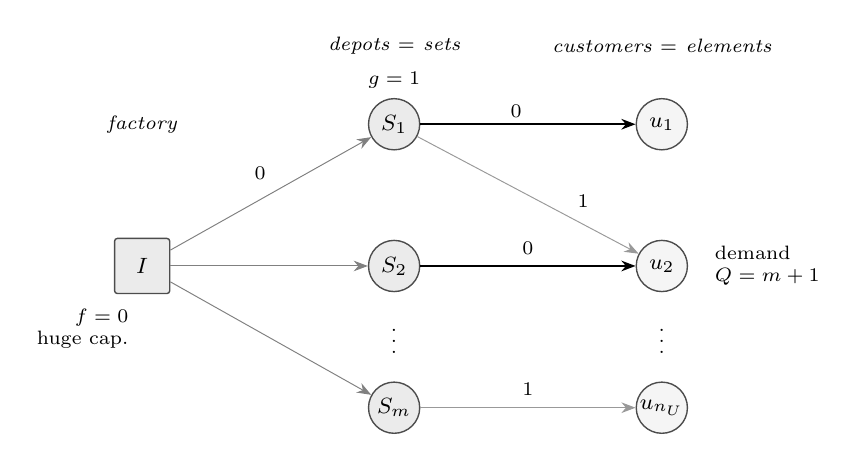
\begin{tikzpicture}[
      >={Stealth[length=1.8mm]},
      every node/.style={font=\footnotesize},
      fac/.style={draw=black!70,line width=0.5pt,fill=black!8,rounded corners=1pt,minimum size=7mm,inner sep=1pt},
      dep/.style={draw=black!70,line width=0.5pt,circle,fill=black!8,minimum size=6.5mm,inner sep=0pt},
      cus/.style={draw=black!70,line width=0.5pt,circle,fill=black!4,minimum size=6.5mm,inner sep=0pt},
      s1/.style={draw=black!50,line width=0.35pt,->},
      cost0/.style={draw=black,line width=0.9pt,->},
      cost1/.style={draw=black!40,line width=0.35pt,->}
    ]
    % factory
    \node[fac] (I) at (0,1.2) {$I$};
    \node[font=\scriptsize,anchor=north east,align=right] at (-0.05,0.78) {$f=0$\\ huge cap.};
    % depots = sets
    \node[dep] (s1) at (3.2,3.0) {$S_1$};
    \node[dep] (s2) at (3.2,1.2) {$S_2$};
    \node[dep] (sm) at (3.2,-0.6) {$S_m$};
    \node[font=\scriptsize,anchor=south] at (s1.north) {$g=1$};
    \node[font=\scriptsize] at (3.2,0.35) {$\vdots$};
    % customers = universe
    \node[cus] (u1) at (6.6,3.0) {$u_1$};
    \node[cus] (u2) at (6.6,1.2) {$u_2$};
    \node[cus] (un) at (6.6,-0.6) {$u_{n_U}$};
    \node[font=\scriptsize] at (6.6,0.35) {$\vdots$};
    \node[font=\scriptsize,anchor=west,align=left] at (7.15,1.2) {demand\\ $Q=m+1$};
    % layer captions
    \node[font=\scriptsize\itshape] at (0,3.0) {factory};
    \node[font=\scriptsize\itshape] at (3.2,4.0) {depots $=$ sets};
    \node[font=\scriptsize\itshape] at (6.6,4.0) {customers $=$ elements};
    % stage-1 arcs cost 0
    \foreach \b in {s1,s2,sm}{\draw[s1] (I) -- (\b);}
    \node[font=\scriptsize] at (1.5,2.38) {$0$};
    % stage-2: solid cost 0 (u in S), faint cost 1 (u notin S)
    \draw[cost0] (s1) -- (u1); \node[font=\scriptsize] at (4.75,3.17) {$0$};
    \draw[cost0] (s2) -- (u2); \node[font=\scriptsize] at (4.9,1.43) {$0$};
    \draw[cost1] (s1) -- (u2); \node[font=\scriptsize] at (5.6,2.02) {$1$};
    \draw[cost1] (sm) -- (un); \node[font=\scriptsize] at (4.9,-0.36) {$1$};
  \end{tikzpicture}%
  }
  \caption{The Set Cover reduction behind Theorem~\ref{thm:cover}, with
  a single product and a single free factory of ample capacity. Each
  depot is a set $S_j$ with opening cost $1$, each customer is a
  universe element with demand $Q=m+1$, and a heavy stage-2 arc costs
  $0$ when the element lies in the set while a light arc costs $1$.
  Opening a depot is choosing its set into the cover, an uncovered
  element can be served only at cost at least $Q>B$, and the budget
  $B=t$ is therefore attainable exactly when a cover of size $t$
  exists.}
  \label{fig:coverage}
\end{figure}


\begin{theorem}\label{thm:cover}
$\mathrm{MP\text{-}TSCFLP}(B)$ is strongly NP-hard even when,
simultaneously, $|L|=1$ and $|I|=1$, the charges satisfy $f\equiv 0$ and
$g\equiv 1$, all transport costs lie in $\{0,1\}$, with in fact
$c\equiv 0$ and $d\in\{0,1\}$, and every number of the instance is bounded
by $|K|\,(|J|+1)$. In particular the problem is NP-hard already under a
unary encoding of the data.
\end{theorem}

We sketch the reduction before giving the formal proof. From an
instance of \textsc{Set Cover} with universe $U$, family
$\mathcal S=\{S_1,\dots,S_m\}$ and target $t$ we build one depot per set,
one customer per element with demand $Q=m+1$, and a single free factory
of ample capacity. The second-stage cost $d_{ju}$ is zero when
$u\in S_j$ and one otherwise, so a customer whose element is covered by
some open depot is served for free, while a customer left uncovered pays
one unit on every unit of its demand and therefore at least $Q$. Since
$Q=m+1$ exceeds both the number of depots and the target $t$, a solution can
stay within budget $B=t$ only if its open depots cover $U$, and then its
cost is exactly the number of open depots. Deciding whether budget $t$ is
attainable is thus deciding whether a cover of size $t$ exists. The
amplifier $Q$ is what makes an uncovered element incompatible with the
budget, and the per-unit accounting is what keeps
divisible service from diluting the penalty.

\begin{proof}
The plan follows the sketch, with the amplifier making the accounting
exact. We reduce from \textsc{Set Cover}, which is NP-complete
\citep{Karp1972}, under the harmless convention $1\le t\le m$. The
remaining values of $t$ are decidable in polynomial time, since an
instance with $t=0$ is a yes-instance exactly when $U=\emptyset$, while
an instance with $t>m$ is a yes-instance exactly when
$\bigcup_j S_j\supseteq U$. The nondegeneracy convention guarantees in
addition that every cover of $U$ is nonempty.

\emph{Construction.} Put $L=\{1\}$ and $I=\{1\}$ with $f_1=0$ and
capacity $b_1=n_U Q$, where $n_U=|U|$ and $Q=m+1$. Take one depot per
set, $J=\{1,\dots,m\}$ with $g_j=1$ and $p_j=n_U Q$, and one customer per
element, $K=U$ with demand $q_u=Q$. Set $c_{1j}=0$ for every $j$, set
$d_{ju}=0$ when $u\in S_j$ and $d_{ju}=1$ otherwise, and ask whether
$\OPT\le B=t$. The construction runs in $O(n_U m)$ time and its largest
number is $n_U(m+1)\le|K|(|J|+1)$.

\emph{Feasibility.} By Proposition~\ref{prop:feas} a design that opens the
factory and a depot set $Z$ is feasible if and only if $b_1\ge D_1$ and
$\sum_{j\in Z}p_j\ge D_1$, where the single product has total demand
$D_1=\sum_u q_u=n_U Q$. Since $b_1=n_U Q$ and each $p_j=n_U Q$, (F1) holds
whenever the factory is open and (F2) holds whenever $Z\ne\emptyset$.
Positive demand, guaranteed by the nondegeneracy convention, forces the
factory open, so the feasible designs are
exactly those with $Z\ne\emptyset$, and the empty design is infeasible.

\emph{Correctness.} Let $Z\subseteq J$ be the depots opened by a feasible
solution. Because $f_1=0$ and $c\equiv 0$, its cost equals
$|Z|+\sum_{j\in Z}\sum_{u\notin S_j}w_{ju}$, the transport sum ranging
over open depots because a closed depot forwards nothing
by~\eqref{eq:C4}. By constraint~\eqref{eq:C1} every unit sent to an
uncovered customer travels on an arc of cost one, so the cost is at least
$|Z|+Q\cdot V_Z$, where $V_Z$ counts the elements no open depot covers.
This lower bound holds for arbitrary divisible flows, since the second
term is charged one unit per unit of flow and an uncovered customer has
no cheaper arc available. It is attained by routing each covered
customer through a covering depot and each uncovered one through any open
depot, with the first-stage flow $x_{1j}$ set to the outflow of depot
$j$, a choice that costs nothing since $c\equiv 0$. The capacities
accommodate this routing, because $b_1=p_j=n_UQ$ equals the total demand
and so \eqref{eq:C2}--\eqref{eq:C4} hold. Now, if $C$ covers
$U$ with $|C|\le t$, then $C$ is nonempty by the nondegeneracy
convention, so opening $Z=C$ is feasible and serves every customer
for free at cost $|C|\le t$. Conversely a solution of cost at most $t$ cannot leave an
element uncovered, for that would force cost at least
$|Z|+Q\ge Q=m+1>m\ge t$, so its open depots form a cover, and
$\text{cost}\ge|Z|$ gives $|Z|\le t$. Neither direction used any
restriction beyond the budget, a fact that Theorem~\ref{thm:w2} reuses
when a cardinality bound is added.

All numbers are bounded by $n_U(m+1)$ and hence polynomial in the input
size, so the subclass remains NP-hard when its data are written in
unary, which is strong NP-hardness in the sense of
\citet{GareyJohnson1979}. A pseudo-polynomial algorithm would run in
polynomial time on this subclass, whose numbers are polynomially
bounded, and would therefore give $\Ppoly=\NP$.
\end{proof}

For coverable instances the value of the reduced instance equals the
minimum cover size, so the approximation threshold of \textsc{Set Cover} transfers verbatim.
The only care needed is that a multiplicative factor below one is
unsatisfiable once the optimum is at least one, which holds here because
a depot must open, and this is why the factor is stated as a maximum
with one.

\begin{corollary}\label{cor:coverinapprox}
For every $\varepsilon>0$, unless $\Ppoly=\NP$, no polynomial-time
algorithm approximates the optimisation version of MP-TSCFLP within a
factor $\max\{1,(1-\varepsilon)\ln|K|\}$, even with $|L|=|I|=1$,
$f\equiv 0$, $g\equiv 1$, $c\equiv 0$, $d\in\{0,1\}$ and all numbers
polynomially bounded in the instance size. The same conclusion follows under the stronger
assumption $\NP\not\subseteq\mathrm{DTIME}(n^{O(\log\log n)})$ from the
earlier bound of \citet{Feige1998}.
\end{corollary}

\begin{proof}
Enlarging the amplifier forces even approximately optimal solutions to
be covering. Rerun the construction with the
larger amplifier $Q'=n_U m+m+1$, so that $q_u=Q'$ and $b_1=p_j=n_UQ'$,
whose only effect is to widen the penalty. The cost identity of
Theorem~\ref{thm:cover}, namely that any feasible solution costs at
least $|Z|+Q'\,V_Z$ with equality for the routing described there, is
unchanged. The optimum of a coverable instance therefore equals its
minimum cover size $t^*$, attained by covering designs, since any
non-covering design costs at least $Q'$ and $Q'>m\ge t^*$ prevents it
from being optimal. Write
$\rho=\max\{1,(1-\varepsilon)\ln n_U\}$ for the claimed factor, and note
$\rho\le 1+\ln n_U$ and $t^*\le m$, so a $\rho$-approximation returns a
solution of cost at most $\rho\,t^*\le(1+\ln n_U)\,m$. Since $\ln n_U<n_U$
this is below $Q'=(n_U+1)m+1$, so the returned design is covering. The
returned solution costs at least $|Z|$ by the identity, where
$Z$ denotes its open depots, so $|Z|\le\rho\,t^*$. As
$|K|=|U|=n_U$, this yields a polynomial-time approximation of factor
$\rho$ for minimum set cover on the coverable instances. The hardness of
\citet{DinurSteurer2014} concerns exactly that minimisation problem,
whose instances are coverable by definition, since a cover is required
for the objective to exist. On instances with $(1-\varepsilon)\ln n_U<1$ the
universe has constant size at most $e^{1/(1-\varepsilon)}$, every
minimal cover has at most $n_U$ sets, and exhaustive search over the
polynomially many subfamilies of at most $n_U$ sets solves the problem
exactly in polynomial time. On all remaining instances
$\rho=(1-\varepsilon)\ln n_U$, so the combined algorithm achieves the
factor $\max\{1,(1-\varepsilon)\ln|U|\}$ on every instance of minimum
set cover, exactly on the small universes and within
$(1-\varepsilon)\ln|U|$ elsewhere. In either regime the combined
procedure would approximate minimum set cover within a factor smaller
than the threshold of \citet{DinurSteurer2014} on every instance, and
that is impossible unless $\Ppoly=\NP$. The
variant under Feige's assumption is identical.
\end{proof}

Fixing a set to a single element removes tractability entirely rather
than merely obstructing efficiency, which is the parameterized reading of the
same reduction.

\begin{corollary}\label{cor:coverpara}
$\mathrm{MP\text{-}TSCFLP}(B)$ is para-NP-hard with respect to $|L|$,
with respect to $|I|$, and with respect to the pair $(|L|,|I|)$. Unless
$\Ppoly=\NP$, none of these parameters admits an \XP\ algorithm, and a
fortiori none is \FPT.
\end{corollary}

\begin{proof}
The claims follow from the fixed slice. The hard subclass of
Theorem~\ref{thm:cover} has $|L|=|I|=1$, so a fixed
slice of each parameter is already NP-hard. A parameterized problem
NP-hard at a fixed parameter value is para-NP-hard, and an \XP\ algorithm
would decide that slice in polynomial time \citep{DowneyFellows2013}.
\end{proof}

Before the covering elements migrate to other dimensions of the model,
we record what the uniform costs of the construction do and do not imply.

\begin{remark}\label{rem:ufl}
The uniformity in Theorem~\ref{thm:cover} is deliberate. All of the
difficulty is already present with $f\equiv 0$, $g\equiv 1$ and binary
transport, so parameters counting distinct cost values, or bounding the ratio of the
positive costs, are constant on this hard subclass and help nothing on
their own. The instance is, in essence, a
non-metric uncapacitated facility location problem with a free source
stage attached, and its equivalence with \textsc{Set Cover} traces back
to \citet{Hochbaum1982}. What the theorem contributes is not the
technique but the location of the difficulty in the most restricted
subclass the model contains.
\end{remark}

\subsection{Products and customers as covering elements}\label{sec:products}

Theorem~\ref{thm:cover} kept the customers as the covering elements and
let the depots do the discriminating, but nothing forces that assignment.
If the products carry the elements and the factories discriminate through
their first-stage costs, the same amplifier argument reaches a group of
instances that Theorem~\ref{thm:cover} cannot, namely one where the
customers collapse to a single point. The hypotheses stay just as tight,
and the difficulty is now carried by the product dimension.

\begin{theorem}\label{thm:products}
$\mathrm{MP\text{-}TSCFLP}(B)$ is strongly NP-hard even when,
simultaneously, $|J|=|K|=1$, the charges satisfy $f\equiv 1$ and $g_1=0$,
first-stage costs lie in $\{0,1\}$ while second-stage costs vanish, and
every number is bounded by $|I|+1$.
The difficulty is carried by $|L|$, which remains unrestricted.
\end{theorem}

The elements have migrated from the customers to the products and
the discriminating layer from the depots to the factories, which is what
moves the hard group to $|J|=|K|=1$.

\begin{proof}
Again the source is \textsc{Set Cover} \citep{Karp1972}, with
$1\le t\le m$ and $Q=m+1$.

\emph{Construction.} Let $L=U$ and $I=\{1,\dots,m\}$ with $f_i=1$ and
$b_{il}=Q$ for every $l$. Take one depot with $g_1=0$ and $p_{1l}=Q$, one
customer with $q_{1l}=Q$, first-stage cost $c_{i1l}=0$ when $l\in S_i$
and $1$ otherwise, second-stage cost $d\equiv 0$, and budget $B=t$. The
construction takes $O(n_U m)$ time, since each cost $c_{i1l}$ is a
membership test. Full
capacity on every product makes feasibility of a design independent of
coverage, so coverage is punished only in the cost.

\emph{Correctness.} By Proposition~\ref{prop:feas}, applied per product
with $b_{il}=p_{1l}=Q$ and $D_l=q_{1l}=Q$, a design $(Y,z_1)$ is feasible
exactly when $Y\ne\emptyset$ and $z_1=1$. Products exist because
$L=U\ne\emptyset$ under the nondegeneracy convention, and for each
product (F1) reads $Q|Y|\ge Q$ and holds precisely when
$Y\ne\emptyset$, while (F2) reads $Qz_1\ge Q$ and forces $z_1=1$, an
opening that is free since $g_1=0$.
A feasible solution with open factories $Y$ and $z_1=1$ costs
$|Y|+\sum_l\sum_{i\in Y,\,l\notin S_i}x_{i1l}$, where the sum ranges over
open factories only, by~\eqref{eq:C3}. For each product the depot must receive $Q$ units
by~\eqref{eq:C1}--\eqref{eq:C2}. If no open factory contains that product
all $Q$ units travel on cost-one arcs, so the cost is at least
$|Y|+Q\,V_Y$, where $V_Y$ counts uncovered products. Equality is
attained by routing each covered product through a containing factory
and each uncovered product through any open factory, within the
per-product capacities $b_{il}=Q$, and the second stage forwards the $Q$
units to the customer at no charge. In
the forward direction a cover $C$ opens $Y=C$ and $z_1=1$ at cost
$|C|\le t$. Conversely a solution of cost at most $t<Q$ leaves no product
uncovered, since one uncovered product would force cost at least
$|Y|+Q\ge 1+Q>m\ge t$, feasibility having forced $Y\ne\emptyset$, and
then $\text{cost}\ge|Y|$ gives $|Y|\le t$, a cover. The
largest number is $Q=m+1$, so the hardness is strong
\citep{GareyJohnson1979}.
\end{proof}

The stages of the model are not interchangeable, because the balance
constraint~\eqref{eq:C2} orients the flow, so the mirror image with
depots as the discriminating layer needs its own short argument rather
than a symmetry appeal.

\begin{corollary}\label{cor:mirror}
$\mathrm{MP\text{-}TSCFLP}(B)$ is strongly NP-hard even when,
simultaneously, $|I|=|K|=1$, the charges satisfy $f_1=0$ and $g\equiv 1$,
first-stage costs vanish while second-stage costs lie in $\{0,1\}$, and
every number is bounded by $|J|+1$.
\end{corollary}

\begin{proof}
The construction of Theorem~\ref{thm:products} transfers across the two
stages, and the proof is the following list of changes. Exchange the
two facility layers, so the sets become depots $J=\{1,\dots,m\}$ with
$g_j=1$ and $p_{jl}=Q$, the single free facility becomes a factory with
$f_1=0$ and $b_{1l}=Q$, and the penalty moves onto the second stage,
$c\equiv 0$ and $d_{j1l}=0$ when $l\in S_j$ and $1$ otherwise, with
$L=U$, the demands $q_{1l}=Q$, the budget $B=t$ and the construction
time unchanged. In the correctness argument the two feasibility tests
swap parts, (F1) reading $Qy_1\ge Q$ and forcing $y_1=1$ at no charge,
(F2) reading $Q|Z|\ge Q$, that is $Z\ne\emptyset$. The cost of a
feasible solution becomes
$|Z|+\sum_l\sum_{j\in Z,\,l\notin S_j}w_{j1l}$ with the sum over open
depots by~\eqref{eq:C4}, and the lower bound $|Z|+Q\,V_Z$, with $V_Z$
the number of uncovered products, holds as before, each product's $Q$
units reaching the customer by~\eqref{eq:C1}. Equality is attained by
the routing of Theorem~\ref{thm:products} with each first-stage flow
$x_{1jl}$ set equal to $w_{j1l}$, at no cost since $c\equiv 0$, within
$b_{1l}=Q$ and satisfying \eqref{eq:C2} and~\eqref{eq:C3}. The two
directions of the equivalence then read verbatim with $Y$ replaced by
$Z$, one uncovered product forcing cost at least $1+Q>m\ge t$. Every
number of the image is again at most $Q=m+1$, so the reduction is
unary-robust and strong NP-hardness follows \citep{GareyJohnson1979}.
\end{proof}

Because these slices are strongly hard, the customer and depot parameters
already fail at the value one, and unlike the weak slice below the
difficulty does not vanish under a unary encoding.

\begin{corollary}\label{cor:parak}
$\mathrm{MP\text{-}TSCFLP}(B)$ is strongly para-NP-hard with respect to
$|K|$, to $|J|$, and to each of the pairs $(|J|,|K|)$ and $(|I|,|K|)$. No
\XP\ algorithm exists for any of these parameters unless $\Ppoly=\NP$, and
every one of these exclusions holds even under a unary encoding.
\end{corollary}

\begin{proof}
Two fixed slices supply the claims.
Theorem~\ref{thm:products} gives a strongly NP-hard slice with
$|J|=|K|=1$ and $|L|$ free, and Corollary~\ref{cor:mirror} one with
$|I|=|K|=1$. The parameterized reading is that of
Corollary~\ref{cor:coverpara}.
\end{proof}

Where no facility layer sees a demand dimension it can distinguish, the
covering mechanism becomes inactive and only the numbers remain hard. This
happens exactly with one depot and one product, and there the difficulty
drops from strong to weak.

\begin{theorem}\label{thm:partition}
$\mathrm{MP\text{-}TSCFLP}(B)$ is NP-hard even when $|J|=|L|=|K|=1$,
$g_1=0$, all transport costs vanish, and $f_i=b_i$ for every factory.
The hardness is only weak, since this group of instances is solvable in
pseudo-polynomial time $O(|I|\cdot(D+b_{\max}))$ with $D=q_{11}$ and
$b_{\max}=\max_i b_i$, and is therefore in $\Ppoly$ under a unary
encoding, hence not strongly NP-hard unless $\Ppoly=\NP$.
\end{theorem}

\begin{proof}
The reduction is from \textsc{Partition}
\citep{Karp1972}, which asks whether
integers $a_1,\dots,a_m$ with even sum $A$ admit a subset summing to
$A/2$, and the matching pseudo-polynomial program follows it.

\emph{Construction.} Take $L=K=\{1\}$ with demand $q=A/2$, one factory
per item with $f_i=b_i=a_i$, one depot with $g_1=0$ and $p_1=A/2$, all
transport costs zero, and budget $B=A/2$.

\emph{Correctness.} Every transport coefficient is zero and $g_1=0$, so
the cost of any feasible solution is $\sum_{i\in S}a_i$ with $S$ the open
factories. By Proposition~\ref{prop:feas} the design is feasible exactly
when $z_1=1$ and $\sum_{i\in S}a_i\ge A/2$. The first condition is
forced by (F2), which reads $p_1z_1=(A/2)z_1\ge A/2$ with $A>0$ by the
nondegeneracy convention, and the opening carries no charge. The second
condition is (F1). A partition $S^\ast$ opens a
feasible solution of cost exactly $A/2$, and a feasible solution of cost
at most $A/2$ has $\sum_S a_i\ge A/2$ and $\le A/2$, hence a partition. The instance
numbers are the $a_i$ themselves, written in binary, so the reduction is
not unary-robust and the hardness is only weak
\citep{GareyJohnson1979}.

\emph{The matching program.} On the general group of the statement the
depot capacity $p_1$ is arbitrary, so we first test $p_1\ge D$ in $O(1)$
time and declare the instance infeasible when the test fails. When it
holds the depot opens at no charge, the cost of opening $S$
is $\sum_{i\in S}f_i=\sum_{i\in S}b_i$, and feasibility is
$\sum_{i\in S}b_i\ge D$ by Proposition~\ref{prop:feas}, so the problem is
the knapsack-cover of minimising a subset sum subject to reaching $D$.
Let $T(i,s)\in\{0,1\}$ record whether some subset of the first $i$
factories has capacity sum exactly $s$, for $0\le s\le D+b_{\max}$. Sums
beyond $D+b_{\max}$ are irrelevant, for if a feasible $S$ has
$\sum_{i\in S}b_i\ge D+b_{\max}$ then removing any item of $S$ keeps the
sum at least $D$, so repeated removal produces a feasible subset of no
larger cost whose sum lies below $D+b_{\max}$. The recurrence
$T(i,s)=T(i-1,s)\vee T(i-1,s-b_i)$, with $T(0,0)=1$, with $T(0,s)=0$ for
$s>0$, and with the convention $T(i-1,s-b_i)=0$ when $s<b_i$, fills the
table in $O(|I|\cdot(D+b_{\max}))$ time. By induction on $i$ the
recurrence is sound and complete, every set bit corresponding to a
genuine subset sum and every subset sum in range setting its bit. The
optimum is the least $s\ge D$ with $T(|I|,s)=1$, and if no such $s$
exists the instance is infeasible, since the removal argument above
would otherwise produce a feasible sum within the range of the table.
The table
is pseudo-polynomial, so under a unary encoding this group lies in
$\Ppoly$ and the weak hardness is best possible.
\end{proof}

The same weak reduction runs with the two facility layers exchanged, which is
what closes the last quadrant of the dichotomy, the one that keeps the depots
free.

\begin{corollary}[depot mirror of the weak group]\label{cor:partitionmirror}
$\mathrm{MP\text{-}TSCFLP}(B)$ is NP-hard even when $|I|=|L|=|K|=1$, $f_1=0$, all
transport costs vanish, and $g_j=p_j$ for every depot. The hardness is only weak,
since this group is solvable in pseudo-polynomial time and hence lies in
$\Ppoly$ under a unary encoding.
\end{corollary}
\begin{proof}
Exchanging the two facility layers in the construction of
Theorem~\ref{thm:partition} yields the reduction, and the proof is the
list of changes. The items become depots with $g_j=p_j=a_j$, the single
free depot becomes a factory with $f_1=0$ and $b_1=A/2$, and the
customer, the demand $q=A/2$, the zero transport costs and the budget
$B=A/2$ are unchanged. In the correctness argument the two feasibility
tests swap parts, (F1) reading $b_1y_1=(A/2)y_1\ge A/2$ with $A>0$ by
the nondegeneracy convention, forcing the free factory opening, and
(F2) supplying the covering test $\sum_{j\in Z}a_j\ge A/2$ over the
open depots $Z$. The equivalence between solutions of cost at most
$A/2$ and partitions then reads word for word as in
Theorem~\ref{thm:partition} with $Z$ in place of $S$. The instance
numbers are the $a_j$ in binary, so the reduction is not unary-robust.
The dynamic program of Theorem~\ref{thm:partition}, run with
$g_j=p_j=a_j$ in place of $f_i=b_i$ after the $O(1)$ test $b_1\ge D$,
whose failure means infeasibility,
places the group in $\Ppoly$ under a unary encoding \citep{GareyJohnson1979}.
\end{proof}

Together the two weak slices delimit the quadrant of the model in which
the covering layer is silent, and the next observation makes that
delimitation explicit.

\begin{observation}\label{obs:quadrant}
With $|J|=|L|=1$ and $|I|,|K|$ free the covering layer is entirely
inactive. Through a single depot the factories cannot tell customers
apart, and a single product offers no dimension to discriminate either,
so the group of instances is at once weakly NP-hard, by
Theorem~\ref{thm:partition}, and pseudo-polynomially solvable. With one
product and one depot every unit of every $q_{k}$ crosses the same depot
to its customer, so the second-stage cost of any trimmed routing is the fixed constant
$\sum_k d_{1k}q_{k}$, independent of the design. Feasibility further
requires $p_1\ge\sum_k q_k$, an $O(1)$ test supplied by (F2) whose
failure means the instance is infeasible, and when the total demand is
positive the forced opening $z_1=1$ adds the constant charge $g_1$ to
every solution. What remains is a
factory-side knapsack-cover with opening charges $f_i$ and per-unit costs
$c_{i1}$ against demand $\sum_k q_k$, solvable in pseudo-polynomial time
by the factory half of the dynamic program behind
Theorem~\ref{thm:separable}, of which the subset-sum of
Theorem~\ref{thm:partition} is the special case $f_i=b_i$, $c\equiv 0$. This is the only quadrant we identify with such
a mixed profile, and it witnesses the two-layer picture directly. The
covering layer becomes active only when a facility layer sees a demand
dimension that distinguishes its members, and where none does the numeric
layer alone remains, vanishing under a unary encoding.
\end{observation}

\subsection{The parameter \texorpdfstring{$k$}{k}}\label{sec:paramk}

The genuine parameter of the study is the number of opened facilities
$k=\sum_i y_i+\sum_j z_j$ of Definition~\ref{def:Bk}, and the covering
reductions already say what to expect of it. \textsc{Set Cover}
parameterized by the cover size is the canonical W[2]-complete problem,
and the construction of Theorem~\ref{thm:cover} maps that parameter
almost onto $k$. The only subtlety is that the forced free factory
consumes one unit of cardinality without consuming budget.

\begin{theorem}\label{thm:w2}
$\mathrm{MP\text{-}TSCFLP}(B,k)$ parameterized by $k$ is W[2]-hard, even
on the subclass of Theorem~\ref{thm:cover}. The same reduction shows that
the budget-only version $\mathrm{MP\text{-}TSCFLP}(B)$ parameterized by
$B$ is W[2]-hard, and that the variant whose cardinality bound counts only depots, requiring
$\sum_j z_j\le k_z$, is W[2]-hard with parameter $k_z$, the reduction
setting $k_z=t$.
\end{theorem}

The budget parameterization is W[2]-hard here because the slice carries
unit depot charges, so the budget counts the open depots, and
parameterization by a budget value is encoding-sensitive in general.

\begin{proof}
We reduce from \textsc{Set Cover} parameterized
by $t$, which is W[2]-complete \citep{DowneyFellows2013}. The map is
that of Theorem~\ref{thm:cover},
computed in polynomial time, with $k=t+1$ a computable function of the
source parameter, so it is an \FPT\ reduction
\citep{DowneyFellows2013,Cygan2015}. For the equivalence, a cover $C$ of
size at most $t$ yields a feasible solution of cost $|C|\le t$ and
cardinality $1+|C|\le t+1$, the factory, forced open by the positive
demand, contributing the extra unit while carrying no charge. Conversely
any witness of the target side
satisfies cost at most $t$ and therefore, by the converse direction of
Theorem~\ref{thm:cover}, opens a cover of size at most $t$. The
cardinality bound only restricts the witnesses and so cannot break this
direction.

\emph{Slack.} In the image, cost at most $B$ forces
$\sum_j z_j\le\sum_j g_j z_j\le\text{cost}\le B$ because $g\equiv 1$ and
the other charges are nonnegative, while $\sum_i y_i=1$ because (F1)
with positive demand forces the single factory open. Every feasible
solution of cost at most $B$ therefore has cardinality at most $B+1$, so
the cardinality bound with $k=B+1$ is vacuous. For the budget-only version
the same instance with parameter $B=t$ is already a reduction, for its
equivalence is verbatim that of Theorem~\ref{thm:cover}, whose two
directions used only the budget. For the depot-only variant set
$k_z=t$. A cover $C$ yields a solution with $\sum_j z_j=|C|\le t$, and
the bound $k_z$ only restricts the witnesses, so the converse direction
of Theorem~\ref{thm:cover} is unaffected.
\end{proof}

The exponent of the trivial enumeration is linear in $k$, and under the
Exponential Time Hypothesis \citep{ImpagliazzoPaturiZane2001} that linear
exponent cannot be improved,
which pairs with the \XP\ membership of Observation~\ref{obs:xp} to show
that \XP\ is the right home for this parameter.

\begin{theorem}\label{thm:eth}
Assuming the ETH, no algorithm decides
$\mathrm{MP\text{-}TSCFLP}(B,k)$
in time $f(k)\cdot N^{o(k)}$, where $N$ is the instance size and $f$ is
computable, even on the subclass of Theorem~\ref{thm:cover}. Since $N$
and $n=|I|+|J|$ are polynomially related on the image, the $n^{k+O(1)}$
enumeration of Observation~\ref{obs:xp} is optimal up to the constant in
the exponent.
\end{theorem}

\begin{proof}
We compose two maps and track the parameter through the composition.
The first is the closed-neighbourhood embedding of
\textsc{Dominating Set} into \textsc{Set Cover}, whose universe is
$V(G)$ and whose sets are the closed neighbourhoods $N[v]$ for
$v\in V(G)$, so that dominating sets of size $t$ correspond exactly to
covers of size $t$. A one-vertex instance of \textsc{Dominating Set} is
decidable in constant time, so we assume $n_G\ge 2$, where $n_G$ is the
number of vertices. Composing the embedding with the map of
Theorem~\ref{thm:w2} gives
$\textsc{Dominating Set}(t)\to\mathrm{MP\text{-}TSCFLP}(B{=}t,k{=}t{+}1)$
with an image of size $N\le n_G^{c}$ for an absolute constant
$c$. The size bound follows because the
embedded \textsc{Set Cover} instance has $n_U=m=n_G$, so the image of
the map of Theorem~\ref{thm:cover} consists of an $n_G\times n_G$
second-stage cost table together with numbers bounded by $n_G(n_G+1)$.
Suppose an algorithm decided the image in
time $f(k)\cdot N^{o(k)}$. Substituting $k=t+1$ and $N\le n_G^{c}$ with $c$
constant gives $N^{o(k)}=n_G^{c\cdot o(t+1)}=n_G^{o(t)}$, since a constant
multiple of a sublinear function is sublinear and $o(t+1)=o(t)$, so the
composition would decide \textsc{Dominating Set} in time $f'(t)\cdot
n_G^{o(t)}$ for a computable $f'$, the polynomial cost of the two
reduction steps being absorbed into the product $f'(t)\cdot n_G^{o(t)}$.
This contradicts the ETH lower bound of
\citet{ChenHuangKanjXia2006}, also in \citet[Chapter~14]{Cygan2015}.
Finally, on the image the instance size $N$ and the
facility count $n=|I|+|J|$ satisfy $n\le N\le n^{c'}$ for a constant
$c'$, so an algorithm running in time $f(k)\cdot n^{o(k)}$ would run in
time $f(k)\cdot N^{o(k)}$ and is excluded by the bound just proved,
which makes the $n^{k+O(1)}$ enumeration of Observation~\ref{obs:xp}
optimal up to the constant in the exponent.
\end{proof}

The quantitative form of the exclusion requires one clarification.
Running times of the shape $f(k)\cdot N^{O(k)}$
are not, and could not be, excluded, because the enumeration of
Observation~\ref{obs:xp} achieves exactly such a bound. The excluded
class is fixed before the composition. For every computable $f$ and
every function $h$ with $h(t)/t\to 0$ no algorithm decides the target in
time $f(t)\,N^{h(t)}$, and the composition maps an algorithm with
exponent $h(k)=o(k)$ to one with exponent $h'(t)\le c\,h(t+1)+c$, which
is again $o(t)$. The pair of results thus brackets the parameter from
both sides, the exponent
linear in $k$ being attainable and, under the ETH, optimal.

\begin{remark}\label{rem:w2mem}
Membership in W[2] is left open. A witness is the set of at most $k$
opened facilities, which has the shape W[2] expects, but the acceptance
test compares binary sums and, worse, minimises an internal routing flow
by Proposition~\ref{prop:oracle}, and neither is known to translate into
bounded weft. In particular the natural verifier must evaluate a
minimum-cost flow, a computation that is P-complete in general and is
not known to be expressible by bounded-weft circuits. What can be stated without risk is that
$\mathrm{MP\text{-}TSCFLP}(B,k)$ lies in $\mathrm{W[P]}$, by guessing the
$O(k\log n)$ bits of the opening pattern and verifying in polynomial time,
so the parameter sits between W[2]-hardness and $\mathrm{W[P]}\cap\XP$.
\end{remark}

\subsection{The numeric layer}\label{sec:numeric}

The covering reductions accounted for three of the four ways a facility
layer can discriminate a demand dimension, namely depots against
customers, factories against products, and depots against products. The
remaining question is the group of instances where both demand dimensions
are trivial, $|K|=|L|=1$, and only the general transport matrix couples
the two facility layers. A computational search over small instances and candidate reduction rules,
recorded with the accompanying code, surfaced no tractable structure for this
group, and the explanation is that the group carries a fourth
discrimination pair. Tight capacities turn the factories
themselves into carriers of demand, and the first-stage matrix then
distinguishes factories that no open depot covers.

\begin{theorem}\label{thm:numeric}
$\mathrm{MP\text{-}TSCFLP}(B)$ is strongly NP-hard even when,
simultaneously, $|K|=|L|=1$, the charges satisfy $f\equiv 0$ and
$g\equiv 1$, first-stage costs lie in $\{0,1\}$ while second-stage costs
vanish, capacities are uniform on each side, and every number is bounded
by $|I|\,(|J|+1)$. Consequently this
group of instances admits no pseudo-polynomial algorithm unless
$\Ppoly=\NP$.
\end{theorem}

The discriminating pair is now the two facility layers, mediated by
tight capacities that force every feasible solution to open and
saturate all factories, and both demand dimensions stay fixed at one.

\begin{proof}
The source problem is once more \textsc{Set Cover} \citep{Karp1972},
with $1\le t\le m$ and
$Q=m+1$.

\emph{Construction.} Put $K=L=\{1\}$ with demand $D=n_U Q$, factories
$I=U$ with $f_i=0$ and $b_i=Q$, depots $J=\{1,\dots,m\}$ with $g_j=1$ and
$p_j=n_U Q$, first-stage cost $c_{ij}=0$ when $i\in S_j$ and $1$
otherwise, second-stage cost $d\equiv 0$, and budget $B=t$. As before
the construction takes $O(n_U m)$ time.

\emph{Correctness.} By Proposition~\ref{prop:feas} a design $(Y,Z)$ is
feasible exactly when (F1) $\sum_{i\in Y}b_i=Q|Y|\ge D=Qn_U$, that is
$Y=I$, and (F2) $\sum_{j\in Z}p_j\ge D$, that is $Z\ne\emptyset$, the
second equivalence using $D>0$, guaranteed by the nondegeneracy
convention. Fix a
feasible solution, write $X_j=\sum_i x_{ij}$ for the flow into depot
$j$, and write $w_j=w_{j11}$ for the flow that depot $j$ forwards to the
customer. Summing~\eqref{eq:C1} over the single customer gives $\sum_j w_j\ge D$,
summing~\eqref{eq:C2} over $j$ gives $\sum_j X_j\ge\sum_j w_j$, and
summing~\eqref{eq:C3} over $i$ gives $\sum_j X_j\le\sum_i b_i y_i=Qn_U=D$.
The chain $D\le\sum_j w_j\le\sum_j X_j\le D$ collapses to equalities, so
$\sum_j w_j=\sum_j X_j=D$ and, since each factory ships $\sum_j x_{ij}\le
b_i=Q$ while the total over the $n_U$ open factories is $Qn_U$, each
factory ships exactly $Q$. Moreover $\sum_j (X_j-w_j)=0$ with every
$X_j-w_j\ge 0$ by~\eqref{eq:C2}, so $X_j=w_j$ for all $j$. A closed depot
has $w_j=0$ by~\eqref{eq:C4}, hence $X_j=0$, so no flow enters a closed
depot and the cost sum below runs only over $j\in Z$.

The cost is then
$|Z|+\sum_i\sum_{j\in Z,\,i\notin S_j}x_{ij}$, at least $|Z|+Q\,V_Z$
with $V_Z$ the number of factories no open depot covers, since a factory
$i$ that no open depot covers ships its full load $Q$ on cost-one arcs.
Equality holds by routing each covered factory's load through a covering
depot and each uncovered factory's load through any open depot, at cost
$Q$ for the latter, then setting $w_j=X_j$ at no charge since
$d\equiv 0$, the depot capacities $p_j=n_UQ$ accommodating any inflow.
A cover $C$ opens $Y=I$, forced by (F1) and free since $f\equiv 0$,
together with
$Z=C$ at cost $|C|\le t$. Conversely the amplifier argument of
Theorem~\ref{thm:cover} again shows that a solution of cost at most $t$
leaves no factory uncovered and opens at most $t$ depots. The largest
number is $n_U(m+1)$, polynomial in the input, so the subclass stays
NP-hard when the data are written in unary \citep{GareyJohnson1979}.
\end{proof}

What survives the reduction is exactly the structure of the transport
matrix, and killing that structure restores tractability. When the matrix
is separable the two facility layers decouple and each becomes a
pseudo-polynomial knapsack-cover, so the separable matrices form a
pseudo-polynomially solvable subclass, while
Theorem~\ref{thm:numeric} makes one explicitly non-separable family
strongly hard. The classification of the territory between the two,
including structured non-separable matrices such as low-rank or Monge
matrices, remains open.

\begin{theorem}\label{thm:separable}
On the group $|K|=|L|=1$, if the first-stage matrix is separable, that is
$c_{ij}=\gamma_i+\delta_j$ for integers $\gamma,\delta$ with the arcs
nonnegative, then the problem is solvable in pseudo-polynomial time
$O\bigl(|I||J|+(|I|+|J|)\cdot D\cdot\max(b_{\max},p_{\max})\bigr)$.
Separability is decidable in $O(|I||J|)$ time.
\end{theorem}

The proof, given in \ref{app:tech}, reduces the routing cost to a
function of the two load marginals, realises any consistent pair of
loads by a northwest-corner plan, and solves each facility layer by a
dynamic program over integer loads, integrality of the split optima
coming from the vertex structure of the load polytopes. Separability is
the quadrangle condition $c_{ij}+c_{11}=c_{i1}+c_{1j}$, checked in one
pass over the matrix.

The separable subclass rounds out the numeric layer, and its
parameterized reading closes the account of the group with both demand
dimensions trivial.

\begin{corollary}\label{cor:unary}
$\mathrm{MP\text{-}TSCFLP}(B)$ is strongly para-NP-hard with respect to
the pair $(|K|,|L|)$, and unless $\Ppoly=\NP$ no \XP\ algorithm exists
for it, even under a unary encoding. Under a unary encoding the witness slices of the weak
groups become polynomial, by Theorem~\ref{thm:partition},
Observation~\ref{obs:quadrant} and Theorem~\ref{thm:separable},
while the four covering reductions of
Theorems~\ref{thm:cover}, \ref{thm:products}, \ref{thm:numeric} and
Corollary~\ref{cor:mirror} are unary-robust, so the covering layer
survives unchanged.
\end{corollary}

\begin{proof}
The claims assemble the slices already proved. The slice
$(|K|,|L|)=(1,1)$ is strongly NP-hard by
Theorem~\ref{thm:numeric}, and the parameterized reading is that of
Corollary~\ref{cor:coverpara}, now robust under a unary encoding because
the instance numbers of Theorem~\ref{thm:numeric} are polynomial. For
the remaining claims of the statement, the three positive results match
their slices as follows. The dynamic program of
Theorem~\ref{thm:partition} covers the group $|J|=|L|=|K|=1$, the
knapsack-cover of Observation~\ref{obs:quadrant} covers the quadrant
$|J|=|L|=1$, and Theorem~\ref{thm:separable} covers the separable
part of the group $|K|=|L|=1$. Each of the three runs in
pseudo-polynomial time and hence in polynomial time once the data are
written in unary. The images of the four covering reductions, in
Theorems~\ref{thm:cover}, \ref{thm:products}, \ref{thm:numeric} and
Corollary~\ref{cor:mirror}, carry numbers bounded by $|K|(|J|+1)$,
$|I|+1$, $|I|(|J|+1)$ and $|J|+1$ respectively, so all four remain valid
polynomial-time reductions when their images are encoded in unary.
\end{proof}

Taken together, the reductions of this section show that every way of
bounding a
subset $P\subseteq\{|I|,|J|,|K|,|L|\}$ that fails to retain both facility
layers, that is with $\{|I|,|J|\}\not\subseteq P$, leaves an NP-hard slice, so unless $\Ppoly=\NP$ a tractable
parameterization of this kind must retain $|I|$ and $|J|$ together. Section~\ref{sec:algorithms} takes
up exactly that surviving combination, where the enumeration of
Observation~\ref{obs:xp} sharpens into fixed-parameter tractability.
The exponent of the $n^{k+O(1)}$ enumeration itself cannot be lowered
under the ETH, by Theorem~\ref{thm:eth}.

\section{Parameterized algorithms and kernels}\label{sec:algorithms}

The hardness map of Section~\ref{sec:complexity} is dense, yet it leaves
positive windows, and this section fills them. We give an \XP\ algorithm
in the number of opened facilities, the branch-and-bound
refinement we implement, the fixed-parameter algorithm that pins down the
size-parameter dichotomy, the routing certificates that bridge the
enumeration to the exact formulation, and the two sides of the
kernelization question. A short remark on width parameters closes the
account, and Table~\ref{tab:landscape} then collects the whole landscape.

\subsection{An \XP\ algorithm in the number of opened
facilities}\label{sec:xp}

Once a design is fixed the cost is determined by the routing oracle of
Proposition~\ref{prop:oracle}, so the only combinatorial freedom left is
which facilities to open. Bounding that freedom by $k$ leaves at most
$e\,n^{k}$ candidate supports, with $e$ the base of the natural
logarithm, and each is priced by one oracle call.
The next theorem promotes the brute-force membership of
Observation~\ref{obs:xp} to a running time whose exponent is linear in
$k$, and the branch-and-bound that follows stays within the same
$n^{k+O(1)}$ regime while pruning aggressively in practice.

The \emph{support} of a design is the set of facilities it opens. We
identify each set $S\subseteq I\cup J$ with the design that opens exactly
the facilities of $S$, and under this identification we write $v(S)$ for
its routing value, $f(S)=\sum_{i\in S\cap I}f_i$ and
$g(S)=\sum_{j\in S\cap J}g_j$ for its two fixed charges, and
$\mathrm{cost}(S)=f(S)+g(S)+v(S)$ for its total cost. On an infeasible
support the convention $v(S)=+\infty$ of Section~\ref{sec:prelim}
gives $\mathrm{cost}(S)=+\infty$.

\begin{theorem}\label{thm:xp}
Write $T_{\mathrm{orac}}$ for the time of one routing-oracle call and
normalize $k\le n$. Then $\mathrm{MP\text{-}TSCFLP}(B,k)$ is decidable,
and the least cost $\OPT_k$ over feasible designs opening at most $k$
facilities is computable, in time $O\bigl(n^{k}\cdot
(T_{\mathrm{orac}}+n|L|)+|K||L|\bigr)$ for $k\ge 1$, and in time
$O(T_{\mathrm{orac}}+n|L|+|K||L|)$
for $k=0$, the additive term reading the demand totals once. In particular the problem lies in \XP\ in the parameter $k$.
\end{theorem}
\begin{proof}
A feasible design opening at most $k$ facilities has a
support
$S\subseteq I\cup J$ with $|S|\le k$, its cost is the fixed charge of $S$
plus the routing value $v(S)$, and by Proposition~\ref{prop:oracle} the
routing value is attained, so each feasible support realizes exactly its
cost and $\OPT_k$ is the minimum of $\mathrm{cost}(S)$ over feasible
supports of size at most $k$. When no such support is feasible we put
$\OPT_k=+\infty$, and the correct answer is then \textsc{no}. The totals $D_1,\dots,D_{|L|}$ are computed once in $O(|K||L|)$ time
and reused by every feasibility test, which is the additive term of the
statement. Enumerate
every such $S$, test feasibility
by Proposition~\ref{prop:feas} in $O(n|L|)$ time against the
precomputed totals, and price the feasible
ones by one oracle call. The number of supports is
$\sum_{t=0}^{k}\binom{n}{t}\le\sum_{t=0}^{k}\frac{n^{t}}{t!}
\le n^{k}\sum_{t\ge 0}\frac{1}{t!}=e\,n^{k}$
for $k\le n$ and $k\ge 1$. The middle inequality uses $n^{t}\le n^{k}$
for $t\le k$, valid since $n\ge 1$, and extending the sum adds
nonnegative terms. Each support
costs one $O(n|L|)$ feasibility test plus at most one oracle call, and
$T_{\mathrm{orac}}$ is left as a stated quantity rather than bounded
below, since an implementation may share preprocessed data across calls,
giving $O\bigl(n^{k}(T_{\mathrm{orac}}+n|L|)+|K||L|\bigr)$ in total. For
$k=0$ only the empty design is priced. That design is feasible exactly
when every $D_l=0$, since for it the left-hand sums of (F1) and (F2) are
empty, so one feasibility test and at most one oracle call suffice,
within $O(T_{\mathrm{orac}}+n|L|+|K||L|)$ counting the totals. Comparing the minimum
against $B$ decides $\mathrm{MP\text{-}TSCFLP}(B,k)$.
\end{proof}

\subsection{A practical branch-and-bound refinement}\label{sec:bb}

Theorem~\ref{thm:xp} settles the classification, and the rest is
implementation. The enumeration it counts is wasteful whenever a
partial design already cannot be
completed within the budget, and the branch-and-bound of
Algorithm~\ref{alg:xpbb}, the code the computational study runs,
closes such subtrees early. Its principal device
is a covering count. Because both stages are complete, feasibility of a
product needs only enough open capacity on each side, and a sorted prefix
determines the fewest facilities that supply a demand from a nonnegative
capacity vector.

\begin{lemma}[covering count]\label{lem:cover}
Let $a_1,\dots,a_m\ge 0$ and $D\ge 0$, and let
$a_{(1)}\ge\cdots\ge a_{(m)}$ be the decreasing order. Some $S$ with
$|S|\le s$ has $\sum_{i\in S}a_i\ge D$ if and only if
$\sum_{r\le s}a_{(r)}\ge D$. When $\sum_{r\le m}a_{(r)}<D$ no such $s$
exists and we set $k^\ast(a;D)=+\infty$. Otherwise the least such $s$,
written $k^\ast(a;D)$, is computable by one sort and one prefix scan in
$O(m\log m)$ time, the same scan detecting the infinite case.
\end{lemma}
\begin{proof}
Both directions follow from majorization by the sorted prefix. If
$\sum_{r\le s}a_{(r)}\ge D$ the set of the $s$ largest entries witnesses
the forward direction. Conversely, order any $S$ decreasingly. Its $r$th
element is at most $a_{(r)}$, because the $r$ largest elements of $S$ are
$r$ distinct entries of $a$, each at least that element, so $a$ has at
least $r$ entries at least as large. Summing gives
$\sum_{i\in S}a_i\le\sum_{r\le|S|}a_{(r)}$.
Hence if some $S$ with $|S|\le s$ has $\sum_{i\in S}a_i\ge D$ then
$D\le\sum_{i\in S}a_i\le\sum_{r\le|S|}a_{(r)}\le\sum_{r\le s}a_{(r)}$, the
last step by $a\ge 0$. The prefix sums are nondecreasing in $s$, so the
least $s$ with $\sum_{r\le s}a_{(r)}\ge D$ is found by one sort and one
scan.
\end{proof}

Algorithm~\ref{alg:xpbb} searches over partial designs, and we name the
quantities its nodes carry before giving the listing. A node is a pair
$(O,C)$ in which $O$ is the set of facilities forced open and $C$ the set
forced closed, so that $F=(I\cup J)\setminus(O\cup C)$ collects the free
facilities and $r=k-|O|$ is the remaining cardinality. For a product $l$
let
\[
s_I(l;O,C)=k^\ast\!\Bigl((b_{il})_{i\in F\cap I};\,\max\bigl(0,\,D_l-\textstyle
\sum_{i\in O\cap I}b_{il}\bigr)\Bigr),
\]
the covering count of Lemma~\ref{lem:cover} over the free factory
capacities against the demand left after crediting the already-open
factories, and let
\[
s_J(l;O,C)=k^\ast\!\Bigl((p_{jl})_{j\in F\cap J};\,\max\bigl(0,\,D_l-\textstyle
\sum_{j\in O\cap J}p_{jl}\bigr)\Bigr)
\]
be the analogous count for (F2) over the free depot capacities. The
quantities of line 2 are the root specializations
$k^\ast_I(l)=k^\ast\bigl((b_{il})_{i\in I};D_l\bigr)=s_I(l;\emptyset,\emptyset)$
and
$k^\ast_J(l)=k^\ast\bigl((p_{jl})_{j\in J};D_l\bigr)=s_J(l;\emptyset,\emptyset)$.
Let $v^{\uparrow}=v(O\cup F)$ be the routing value of the all-open
completion, with the convention $v=+\infty$ of
Section~\ref{sec:prelim}, and let $LB(O,C)=f(O)+g(O)+v^{\uparrow}$.
Finally, a facility of $O$ is \emph{unused} by a flow when the flow
carries zero on every arc incident to that facility in every product's
network. Three prunes act on these quantities, and after the listing we
show each is sound and then that the search returns $\OPT_k$.
Figure~\ref{fig:bbtree} places the three prunes on a single branching
step.

% Requires: \usetikzlibrary{positioning,arrows.meta}
\begin{figure}[H]
  \centering
  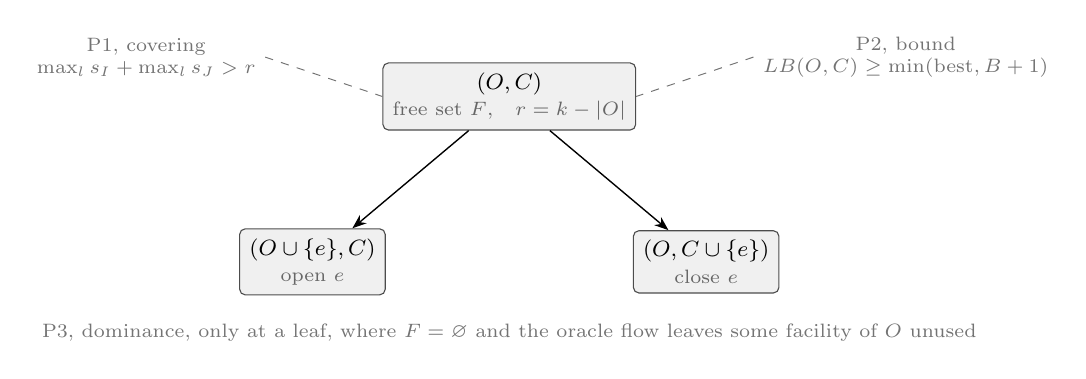
\begin{tikzpicture}[
      >={Stealth[length=1.8mm]},
      res/.style={draw=black!70,line width=0.4pt,fill=black!6,
        rounded corners=2pt,align=center,inner sep=3.5pt,
        font=\footnotesize},
      note/.style={font=\scriptsize,text=black!55,align=center},
      branch/.style={draw=black,line width=0.5pt,->},
      lead/.style={draw=black!55,line width=0.35pt,dashed}
    ]
    \node[res] (P) at (0,0)
      {$(O,C)$\\
       \textcolor{black!60}{\scriptsize free set $F$,\quad $r=k-|O|$}};
    \node[res] (L) at (-2.5,-2.1)
      {$(O\cup\{e\},C)$\\
       \textcolor{black!60}{\scriptsize open $e$}};
    \node[res] (R) at (2.5,-2.1)
      {$(O,C\cup\{e\})$\\
       \textcolor{black!60}{\scriptsize close $e$}};
    \draw[branch] (P) -- (L);
    \draw[branch] (P) -- (R);
    % P1 acts on the popped node, covering counts against r
    \node[note,anchor=east] (p1) at (-3.1,0.5)
      {P1, covering\\ $\max_l s_I+\max_l s_J>r$};
    \draw[lead] (p1.east) -- (P.west);
    % P2 acts on the popped node, admissible bound
    \node[note,anchor=west] (p2) at (3.1,0.5)
      {P2, bound\\ $LB(O,C)\ge\min(\mathrm{best},B+1)$};
    \draw[lead] (p2.west) -- (P.east);
    % P3 acts only at a leaf
    \node[note] (p3) at (0,-3.0)
      {P3, dominance, only at a leaf, where $F=\varnothing$ and the
       oracle flow leaves some facility of $O$ unused};
  \end{tikzpicture}
  \caption{One branching step of Algorithm~\ref{alg:xpbb}. A node
  carries the forced-open set $O$, the forced-closed set $C$, the free
  set $F$ and the remaining cardinality $r$, and branching on a free
  facility $e$ produces the two children along the solid arrows. The
  dashed leaders attach P1 and P2 to the popped node they test, while
  P3 fires only at a leaf, so the three prunes act exactly on the named
  quantities (Lemma~\ref{lem:cover},
  Proposition~\ref{prop:bbcorrect}).}
  \label{fig:bbtree}
\end{figure}


\begin{algorithm}[H]
\caption{Branch-and-bound for $\mathrm{MP\text{-}TSCFLP}(B,k)$
(Theorem~\ref{thm:xp}).}
\label{alg:xpbb}
\begin{pseudolines}
\item $k\gets\min(k,n)$ \algcomment{normalization, no design opens more}
\item \kw{for each} product $l$ sort $(b_{il})_i$ and $(p_{jl})_j$ and
  compute $k^\ast_I(l),k^\ast_J(l)$ \algcomment{Lemma~\ref{lem:cover}}
\item \kw{if}
  $\max_l k^\ast_I(l)+\max_l k^\ast_J(l)>k$ \kw{then} \kw{return}
  \textsc{no} with $\OPT_k=+\infty$
  \algcomment{a priori bound $k^\ast$}
\item $\mathrm{best}\gets+\infty$; push the root $(O,C)=(\emptyset,\emptyset)$
\item \kw{while} the stack is nonempty \kw{do}
\item \algin pop $(O,C)$; let $F$ be the free facilities and
  $r\gets k-|O|$; \kw{if} $r<0$ \kw{then} continue
\item \algin \kw{if}
  $\max_l s_I(l;O,C)+\max_l s_J(l;O,C)>r$ \kw{then} continue
  \algcomment{prune P1, Lemma~\ref{lem:cover}}
\item \algin evaluate the all-open completion by the oracle to get
  $v^{\uparrow}$ and $LB(O,C)$
\item \algin \kw{if} $v^{\uparrow}=+\infty$ \kw{or}
  $LB(O,C)\ge\min(\mathrm{best},B+1)$ \kw{then} continue
  \algcomment{prune P2}
\item \algin \kw{if} $F=\emptyset$ \kw{then}
  \algcomment{leaf, the design is $S=O$}
\item \algin\algin \kw{if} the oracle solution returned at the leaf
  leaves some facility of $O$ unused \kw{then} continue
  \algcomment{prune P3}
\item \algin\algin $\mathrm{best}\gets\min(\mathrm{best},LB(O,C))$
\item \algin \kw{else} pick $e\in F$ of least index and push
  $(O\cup\{e\},C)$ and $(O,C\cup\{e\})$
\item \kw{if} $\mathrm{best}<+\infty$ \kw{and} $\mathrm{best}\le B$
  \kw{then} \kw{return} \textsc{yes} \kw{else} \kw{return} \textsc{no},
  either way reporting $\mathrm{best}$
  \algcomment{run with $B=\infty$ to read $\OPT_k$ off either branch}
\end{pseudolines}
\end{algorithm}

\emph{P1, covering.} Every completion of $(O,C)$ opens $O$ together with
some free facilities. For such a completion $S$ and a product $l$, (F1)
reads $\sum_{i\in S\cap I}b_{il}\ge D_l$, which states that the free
factories of $S$ supply at least the residual demand
$\max(0,D_l-\sum_{i\in O\cap I}b_{il})$, so Lemma~\ref{lem:cover},
applied to $(b_{il})_{i\in F\cap I}$ against that residual demand, shows
that $S$ adds at least $s_I(l;O,C)$ free factories. One open set must
satisfy (F1) for all
products at once, so it adds at least $\max_l s_I(l;O,C)$ free factories,
and likewise at least $\max_l s_J(l;O,C)$ free depots. Factories and depots
are disjoint, so the two increments add, and when their sum exceeds $r$ no
completion has cardinality at most $k$, so P1 discards $(O,C)$ soundly.
An infinite count falls under the same reading, since
$s_I(l;O,C)=+\infty$ means that even opening every free factory leaves
(F1) violated for $l$, so no completion is feasible and the prune fires
for every finite $r$.

\emph{P2, bound.} Any completion opens a set $S$ with $O\subseteq
S\subseteq O\cup F$. Its fixed charge is at least $f(O)+g(O)$ by
nonnegativity of the charges, and its routing
value is at least $v(O\cup F)=v^{\uparrow}$ because $S\le O\cup F$
componentwise and $v$ is monotone (Proposition~\ref{prop:mono}). Hence
$LB(O,C)$ is a lower bound on the cost of \emph{every} completion, even one
opening more than $k$ facilities, which is all the bound needs. P2 discards
$(O,C)$ when $LB(O,C)\ge\min(\mathrm{best},B+1)$, and either threshold
justifies the discard. If $LB(O,C)\ge\mathrm{best}$ then no completion
improves the incumbent. If $LB(O,C)\ge B+1$ then no completion meets the
budget, because the data are nonnegative integers and the routing values
are integers by Proposition~\ref{prop:oracle}, so every cost is an
integer and a cost at most $B$ is a cost strictly below $B+1$. When
$v^{\uparrow}=+\infty$ the same monotonicity gives
$v(S)\ge v(O\cup F)=+\infty$ for every completion $S$, so every
completion is infeasible under the convention of
Section~\ref{sec:prelim} and discarding is again sound. At a
leaf, where $F=\emptyset$, one has $LB(O,C)=\mathrm{cost}(O)$.

\emph{P3, dominance.} When the oracle solution returned at the leaf
leaves an open facility of $O$ unused, closing that facility gives a
design of strictly smaller cardinality. The oracle solution returned at
the leaf carries nothing on any arc of the
closed facility, so it remains a feasible routing of the smaller design,
whence the routing value does not increase, and the fixed charge drops
by the nonnegative charge of that facility. The smaller design is
therefore feasible at no greater cost, so $O$ is dominated and P3
discards it.

With the three prunes justified, the remaining question is whether the
surviving search still reaches an optimum.

\begin{proposition}[correctness]\label{prop:bbcorrect}
Algorithm~\ref{alg:xpbb} decides $\mathrm{MP\text{-}TSCFLP}(B,k)$, and when
run with $B=+\infty$ it returns $\mathrm{best}=\OPT_k$.
\end{proposition}
The full argument appears in Appendix~\ref{app:bb}. Its three steps justify
the early return of line 3 through Lemma~\ref{lem:cover}, bound
$\mathrm{best}$ below by $\OPT_k$ because only feasible designs within
the cardinality budget ever reach a leaf, and bound it above by tracking
a minimum-cardinality optimum down the tree, checking that no prune ever
discards the node carrying it.

The prunes only discard nodes, and the tree they act on is itself
small. Branching always selects the free facility of least index, so at
every node the decided set $O\cup C$ is a prefix of the facility order
and the node is determined by the prefix length $m$ together with
$O\subseteq\{1,\dots,m\}$. Children are pushed only from nodes with
$|O|\le k$, so every node ever created has $|O|\le k+1$ and the tree
holds at most
$\sum_{m=0}^{n}\sum_{t=0}^{k+1}\binom{m}{t}=O(n^{k+2})$ nodes, since
$\sum_{t=0}^{k+1}\binom{m}{t}\le\sum_{t=0}^{k+1}n^{t}\le 2n^{k+1}$
for $n\ge 2$ by the geometric series and the cases $n\le 1$ are
trivial. Each
node performs the sorts and prefix scans of P1 and at most one oracle
call, so the whole search runs in
$O\bigl(n^{k+2}(T_{\mathrm{orac}}+n|L|\log n)+|K||L|\bigr)$ time, with
the additive term again reading the demand totals once, a
polynomial factor above the enumeration bound of Theorem~\ref{thm:xp}
and within the same $n^{k+O(1)}$ regime, which is all the
classification uses. On the seeded validation suite
recorded in the accompanying code, the reference implementation visited
roughly ninety per cent fewer nodes than the plain enumeration and returned
the brute-force optimum on every instance. The
linear exponent is essentially the best one can hope for, since under the
Exponential Time Hypothesis no algorithm decides the problem in time
$f(k)\cdot N^{o(k)}$ (Theorem~\ref{thm:eth}), so the enumeration of
supports is tight up to the constant in the exponent.

One relation among the prunes has consequences that
Section~\ref{sec:exp-q1} meets again on the machine, so we record it
here.

\begin{observation}[the covering prune in plain optimization]
\label{obs:p1redundant}
Run with $k=n$, prune P1 discards no node beyond the infeasibility
branch of P2, since at any node $r=n-|O|=|F|+|C|\ge|F|$. If the
all-open
completion $O\cup F$ is feasible, then for every product the free
facilities of each side supply that side's residual demand, so
Lemma~\ref{lem:cover} gives $\max_l s_I(l;O,C)\le|F\cap I|$ and
$\max_l s_J(l;O,C)\le|F\cap J|$, the two maxima add to at most
$|F|\le r$, and P1 does not fire. When P1 fires, therefore, the
all-open completion is infeasible, so $v^{\uparrow}=+\infty$ and the
infeasibility branch of P2 discards the same node at the price of one
oracle call. Under a binding cardinality $k<n$ the subsumption fails,
since a node may admit a feasible all-open completion while no
completion within the remaining budget $r$ exists, a situation P1 can detect
and the infeasibility branch of P2 cannot.
\end{observation}

\subsection{Fixed-parameter tractability and the size-parameter
dichotomy}\label{sec:fpt}

The parameter $k$ counts openings, whereas the four dimensions
$|I|,|J|,|K|,|L|$ measure the instance itself, and only the two facility
sides carry tractability. Enumerating designs rather than supports gives a
fixed-parameter algorithm in $|I|+|J|$, and coupling it with the hardness
slices of Section~\ref{sec:complexity} pins the exact border that
Figure~\ref{fig:dichotomy} maps over the sixteen subsets.

% Requires: \usetikzlibrary{positioning,fit}
\begin{figure}[H]
  \centering
  \resizebox{0.98\textwidth}{!}{%
  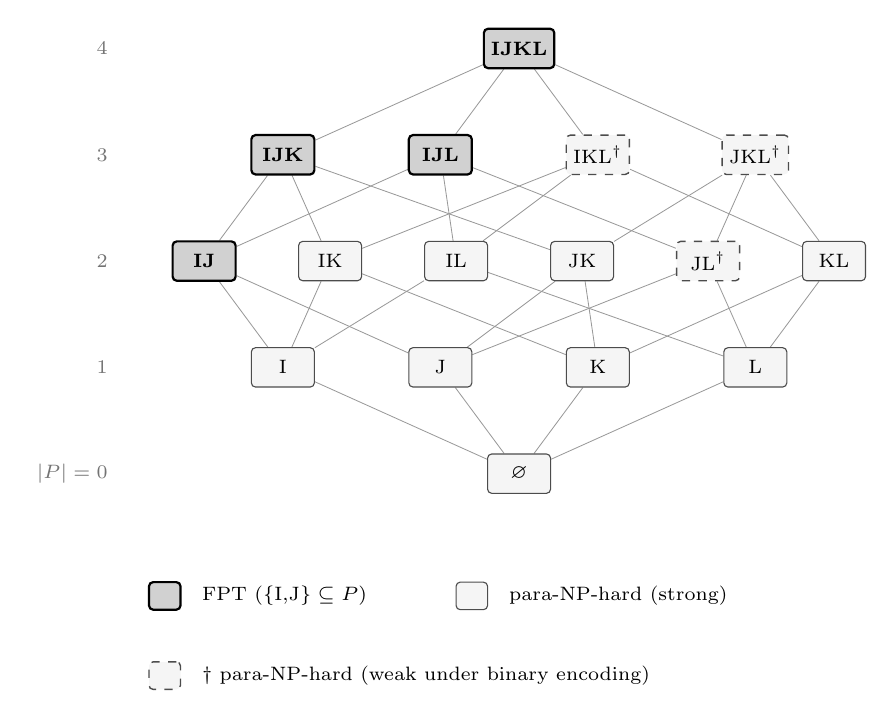
\begin{tikzpicture}[
      x=1cm,y=1.35cm,
      every node/.style={font=\scriptsize},
      nd/.style={draw=black!70,line width=0.4pt,fill=black!4,rounded corners=1.5pt,
        minimum width=8mm,minimum height=5mm,inner sep=2.5pt},
      fpt/.style={draw,line width=0.8pt,fill=black!18,rounded corners=1.5pt,
        font=\scriptsize\bfseries,minimum width=8mm,minimum height=5mm,inner sep=2.5pt},
      weak/.style={draw=black!70,line width=0.5pt,dashed,fill=black!4,rounded corners=1.5pt,
        minimum width=8mm,minimum height=5mm,inner sep=2.5pt},
      ed/.style={draw=black!40,line width=0.3pt}
    ]
    % rank 0
    \node[nd] (e) at (4.5,0) {$\varnothing$};
    % rank 1
    \node[nd] (I) at (1.5,1) {I}; \node[nd] (J) at (3.5,1) {J};
    \node[nd] (K) at (5.5,1) {K}; \node[nd] (L) at (7.5,1) {L};
    % rank 2
    \node[fpt] (IJ) at (0.5,2) {IJ}; \node[nd] (IK) at (2.1,2) {IK};
    \node[nd] (IL) at (3.7,2) {IL}; \node[nd] (JK) at (5.3,2) {JK};
    \node[weak] (JL) at (6.9,2) {JL$^\dagger$}; \node[nd] (KL) at (8.5,2) {KL};
    % rank 3
    \node[fpt] (IJK) at (1.5,3) {IJK}; \node[fpt] (IJL) at (3.5,3) {IJL};
    \node[weak] (IKL) at (5.5,3) {IKL$^\dagger$}; \node[weak] (JKL) at (7.5,3) {JKL$^\dagger$};
    % rank 4
    \node[fpt] (IJKL) at (4.5,4) {IJKL};
    % cover edges (drawn behind)
    \begin{scope}[on background layer]
      \foreach \a/\b in {e/I,e/J,e/K,e/L,
        I/IJ,I/IK,I/IL, J/IJ,J/JK,J/JL, K/IK,K/JK,K/KL, L/IL,L/JL,L/KL,
        IJ/IJK,IJ/IJL, IK/IJK,IK/IKL, IL/IJL,IL/IKL,
        JK/IJK,JK/JKL, JL/IJL,JL/JKL, KL/IKL,KL/JKL,
        IJK/IJKL,IJL/IJKL,IKL/IJKL,JKL/IJKL}{\draw[ed] (\a) -- (\b);}
    \end{scope}
    % rank labels
    \foreach \r/\t in {0/{$|P|=0$},1/{$1$},2/{$2$},3/{$3$},4/{$4$}}{
      \node[anchor=east,font=\scriptsize\itshape,text=black!55] at (-0.6,\r) {\t};}
    % legend
    \begin{scope}[shift={(0,-1.15)}]
      \node[fpt,minimum width=4mm,minimum height=3.5mm] (lf) at (0,0) {};
      \node[anchor=west] at (0.35,0) {FPT ($\{$I,J$\}\subseteq P$)};
      \node[nd,minimum width=4mm,minimum height=3.5mm] (ls) at (3.9,0) {};
      \node[anchor=west] at (4.25,0) {para-NP-hard (strong)};
      \node[weak,minimum width=4mm,minimum height=3.5mm] (lw) at (0,-0.75) {};
      \node[anchor=west] at (0.35,-0.75) {$\dagger$ para-NP-hard (weak under binary encoding)};
    \end{scope}
  \end{tikzpicture}%
  }
  \caption{The size-parameter dichotomy of Theorem~\ref{thm:dichotomy}
  over the sixteen subsets $P\subseteq\{|I|,|J|,|K|,|L|\}$, arranged by
  cardinality as a Hasse diagram whose edges are the cover relations.
  The problem is fixed-parameter tractable exactly on the four
  upward-closed sets that contain both facility layers I and J, shaded
  and shown in bold (Theorem~\ref{thm:fpt}), and para-NP-hard on the
  remaining twelve. Hardness is strong except at the three sets marked
  with a dagger, whose witnessing slices are only weakly NP-hard under a
  binary encoding (Theorem~\ref{thm:partition},
  Corollary~\ref{cor:partitionmirror}).}
  \label{fig:dichotomy}
\end{figure}


\begin{theorem}[fixed-parameter tractability]\label{thm:fpt}
$\mathrm{MP\text{-}TSCFLP}(B)$, its optimization form and its cardinality
version are solvable in time $2^{|I|+|J|}\cdot\mathrm{poly}(N)$, where $N$
is the input size. Hence the problem is \FPT\ in the combined parameter
$(|I|,|J|)$, and a fortiori under any parameter set containing both.
\end{theorem}
\begin{proof}
Enumerate all $2^{|I|+|J|}$ designs, test each by
Proposition~\ref{prop:feas}, price the feasible ones by
Proposition~\ref{prop:oracle}, filter by $\sum y+\sum z\le k$ when the
cardinality bound is present, and return the least cost, compared
against $B$ for the decision versions, reporting infeasibility through
the value $+\infty$ when no design passes the test. Correctness is immediate from the
attainment in Proposition~\ref{prop:oracle}, each step per design runs
in time polynomial in $N$, and the function $2^{|I|+|J|}$ reads only the
two facility counts, which is the definition of \FPT\ in the combined
parameter. The a fortiori clause follows because $2^{|I|+|J|}$ is also a
computable function of any parameter set that contains both facility
counts.
\end{proof}

The synthesis theorem states the border cleanly. For a parameter set $P$
drawn from the four dimensions the problem is fixed-parameter tractable
exactly when $P$ contains both facility sides, and otherwise it is hard
already at a fixed slice.

\begin{theorem}[dichotomy]\label{thm:dichotomy}
Let $P\subseteq\{|I|,|J|,|K|,|L|\}$ parameterize
$\mathrm{MP\text{-}TSCFLP}(B)$. If $\{|I|,|J|\}\subseteq P$ the problem is
\FPT, unconditionally. If $\{|I|,|J|\}\not\subseteq P$ it is
para-\NP-hard, unconditionally, because some assignment of fixed values to
the parameters of $P$ gives an \NP-hard slice, and then no \XP\ algorithm
exists unless $\Ppoly=\NP$. Assuming $\Ppoly\ne\NP$, therefore, the
problem is \FPT\ if and only if $\{|I|,|J|\}\subseteq P$. The same
statement transfers verbatim to $\mathrm{MP\text{-}TSCFLP}(B,k)$ by
appending $k:=n$.
\end{theorem}
\begin{proof}
The positive half is Theorem~\ref{thm:fpt}. For the negative half it
suffices to exhibit, for each of the twelve subsets $P$ with
$\{|I|,|J|\}\not\subseteq P$, an \NP-hard slice that fixes every parameter
of $P$ to the constant one, since a problem \NP-hard at a fixed parameter
value is para-\NP-hard and an \XP\ algorithm would decide that slice in
polynomial time. Six slices from Section~\ref{sec:complexity} cover all
twelve. The slice of Theorem~\ref{thm:cover} fixes $|I|=|L|=1$ and
witnesses $\emptyset$, $\{|I|\}$, $\{|L|\}$ and $\{|I|,|L|\}$. The slice of
Theorem~\ref{thm:products} fixes $|J|=|K|=1$ and witnesses $\{|J|\}$,
$\{|K|\}$ and $\{|J|,|K|\}$, while its mirror, Corollary~\ref{cor:mirror},
fixes $|I|=|K|=1$ and witnesses $\{|I|,|K|\}$. The slice of
Theorem~\ref{thm:numeric} fixes $|K|=|L|=1$ and witnesses $\{|K|,|L|\}$.
The weak slice of Theorem~\ref{thm:partition} fixes $|J|=|K|=|L|=1$ and
witnesses $\{|J|,|L|\}$ and the triple $\{|J|,|K|,|L|\}$, and its depot
mirror, Corollary~\ref{cor:partitionmirror}, fixes $|I|=|K|=|L|=1$ and
witnesses the remaining triple $\{|I|,|K|,|L|\}$. Each of the twelve
subsets with $\{|I|,|J|\}\not\subseteq P$ is contained in one of the six
fixed sets $\{|I|,|L|\}$, $\{|J|,|K|\}$, $\{|I|,|K|\}$, $\{|K|,|L|\}$,
$\{|J|,|K|,|L|\}$, $\{|I|,|K|,|L|\}$, and fixing a superset of $P$ to
constants fixes $P$, so the case analysis is complete. Appending $k:=n$
preserves the answer, because no design opens more than $n$ facilities,
so the appended bound is vacuous and the two problems coincide instance
by instance, and it leaves the fixed values of $P$ untouched.
\end{proof}

Two qualifications attach to the negative half. Para-\NP-hardness
asks only for \NP-hardness of a slice under the standard binary encoding,
and weak hardness already is \NP-hardness, so the weakly hard slices count
towards the dichotomy exactly as the strongly hard ones do. The encoding
matters only when we ask whether the border survives unary numbers. There
the positive half is untouched, and the negative half survives for the
nine parameter sets whose witnessing slices are strongly \NP-hard, while
for $\{|J|,|L|\}$ and the two triples $\{|I|,|K|,|L|\}$ and
$\{|J|,|K|,|L|\}$ the witnessing slices turn polynomial under unary data,
through the pseudo-polynomial programs of Theorem~\ref{thm:partition}
and Corollary~\ref{cor:partitionmirror},
and no other hard slice is known, so their unary status stays open.

\subsection{Certificates and a bridge to the exact
formulation}\label{sec:certificates}

The dichotomy settles what the parameters buy, and this subsection
turns the same oracle into certificates a mixed-integer solver can
consume. Each oracle call solves one transportation problem per product, and its
linear-programming dual both certifies the routing value and supplies a
cut that a Benders master can reuse. The fact that carries the
subsection is that the dual polyhedron depends only on the data, never
on the design, so a single dual point
yields an inequality valid for every design whose block is feasible.
Figure~\ref{fig:bendersflow} traces the pipeline the proposition
formalizes.

% Requires: \usetikzlibrary{positioning,arrows.meta}
\begin{figure}[H]
  \centering
  \resizebox{0.97\textwidth}{!}{%
  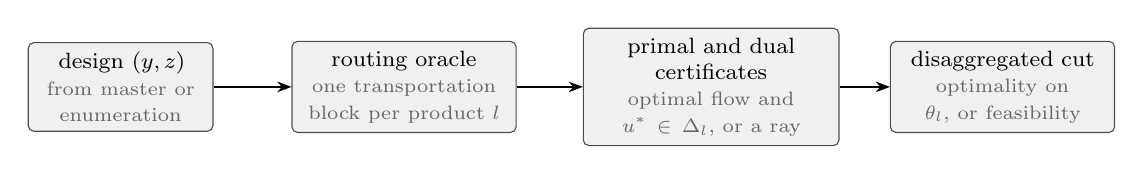
\begin{tikzpicture}[
      >={Stealth[length=1.8mm]},
      res/.style={draw=black!70,line width=0.4pt,fill=black!6,
        rounded corners=2pt,align=center,inner sep=3.5pt,
        font=\footnotesize},
      flow/.style={draw=black,line width=0.5pt,->}
    ]
    \node[res,text width=2.1cm] (D) at (0,0)
      {design $(y,z)$\\
       \textcolor{black!60}{\scriptsize from master or enumeration}};
    \node[res,text width=2.6cm] (O) at (3.6,0)
      {routing oracle\\
       \textcolor{black!60}{\scriptsize one transportation block per
       product $l$}};
    \node[res,text width=3.0cm] (C) at (7.5,0)
      {primal and dual certificates\\
       \textcolor{black!60}{\scriptsize optimal flow and
       $u^\ast\in\Delta_l$, or a ray}};
    \node[res,text width=2.6cm] (K) at (11.2,0)
      {disaggregated cut\\
       \textcolor{black!60}{\scriptsize optimality on $\theta_l$, or
       feasibility}};
    \draw[flow] (D) -- (O);
    \draw[flow] (O) -- (C);
    \draw[flow] (C) -- (K);
  \end{tikzpicture}%
  }
  \caption{From a design to a cut, the pipeline of
  Proposition~\ref{prop:duals}. Each oracle call of
  Proposition~\ref{prop:oracle} prices the design one product at a
  time, returns an optimal flow together with a dual point
  $u^\ast\in\Delta_l$ certifying the block value, and that dual point
  yields the disaggregated Benders optimality cut, valid for every
  design with a feasible block because $\Delta_l$ never depends on $(y,z)$, while an
  infeasible block yields a recession ray and a feasibility cut
  instead.}
  \label{fig:bendersflow}
\end{figure}


\begin{proposition}[routing certificate and Benders cuts]\label{prop:duals}
Fix a product $l$ and let $\Delta_l$ be the dual polyhedron of its
transportation block, which is independent of $(y,z)$. If the block is
feasible then some $u^\ast\in\Delta_l$ attains the dual value
$\mu_l(y,z)$, and the pair of an optimal flow and $u^\ast$ certifies
$\mu_l(y,z)$ in time $O(|I||J|+|J||K|)$. Further, writing $\theta_l$ for
a variable through which a master problem represents the block value, for
every $u=(\alpha,\beta,\sigma,\pi)\in\Delta_l$ the inequality
\[
\theta_l\ \ge\ \sum_k q_{kl}\,\alpha_k
      -\sum_i b_{il}\,\sigma_i\,y_i-\sum_j p_{jl}\,\pi_j\,z_j
\]
is valid for every design whose block $l$ is feasible, and it holds with
equality at the design that generated $u^\ast$. Two explicit recession
rays of $\Delta_l$ certify infeasibility, and their objectives are
positive exactly when (F1), respectively (F2), of
Proposition~\ref{prop:feas} fails.
\end{proposition}
The proof, given in Appendix~\ref{app:duals}, writes the block dual explicitly.
No dual constraint mentions the design, which yields the independence of
$\Delta_l$, weak duality yields the displayed inequality, strong duality
supplies the attaining point $u^\ast$, and the two recession rays are
exhibited coordinate by coordinate and matched to the failures of (F1)
and (F2).

These are precisely the per-product optimality cuts of a disaggregated
Benders decomposition, and the recession rays are its feasibility cuts.
The certificates the enumeration consumes are the objects the Benders
decomposition emits, so each oracle call in Algorithm~\ref{alg:xpbb} can
return, beside its value, the very cut that a branch-and-Benders-cut
master would add at that design. The proposition certifies the routing
value and the validity of the cuts, not the global optimum, which still
needs the master's own bounds.

\subsection{Kernelization}\label{sec:kernel}

Preprocessing is the last algorithmic question, and it divides cleanly.
On the positive side, customers with identical cost columns aggregate
exactly, a bound on costs and total demands yields a polynomial kernel
outright, and a bound on costs and budget still yields a polynomial
compression through the weight-reduction technique of
\citet{FrankTardos1987}. On the negative side, products do not
aggregate, and no polynomial kernel exists in
the winning parameter unless the polynomial hierarchy collapses. The first
reduction is safe and cheap.

\begin{proposition}[customer aggregation]\label{prop:aggregation}
If customers $k\ne k'$ have identical cost columns, that is
$d_{jkl}=d_{jk'l}$ for all $j,l$, then merging $k'$ into $k$ and adding
their demands preserves feasibility, routing value and cost of every
design, hence the optimal value, the set of optimal designs and the
answers of both decision versions. Feasible complete solutions
map in both directions under the explicit merge and split maps of the
proof, which never raise the cost and preserve the optimal routing
value of every design, and consequently one
may assume $|K|\le\tau$, where $\tau$
is the number of distinct second-stage cost columns, computable in
polynomial time.
\end{proposition}
We prove this in Appendix~\ref{app:agg} by exhibiting the two maps directly. The
merge adds the flow rows of the two customers and preserves every
constraint and every cost term. The split trims any surplus of the
merged row and expands it by the northwest-corner procedure, which
preserves feasibility at no cost increase, so the optimal routing
values agree design by design, and a companion reduction bounds the
capacities without touching any design.

\begin{remark}[aggregation up to additive shifts]\label{rem:addshift}
The exact-equality hypothesis can be relaxed at the price of a budget
shift. Suppose the columns of $k$ and $k'$ differ by a product-wise
constant, $d_{jk'l}=d_{jkl}+\alpha_l$ for all $j,l$. In a routing
trimmed as in the proof of Proposition~\ref{prop:aggregation},
customer $k'$ receives exactly $q_{k'l}$ units of product $l$, each
paying $\alpha_l$ more than under the column of $k$ at the same
depot. Replacing the column of $k'$ by that of $k$ therefore shifts
the
routing value of every feasible design by exactly
$-\sum_l\alpha_l q_{k'l}$, and the shift reaches the optima because
they are attained at trimmed routings, trimming never raising the
cost in either instance. The merge of
Proposition~\ref{prop:aggregation} then applies to the now identical
columns once the budget is replaced by
$B-\sum_l\alpha_l q_{k'l}$, the answer being \textsc{no} outright
when that quantity is negative, since costs are nonnegative. We keep
$\tau$ as defined, the refined count of columns distinct up to
product-wise shifts not being needed elsewhere.
\end{remark}

\begin{observation}[capacity capping]\label{obs:capping}
Replacing every capacity $b_{il}$ by $\min(b_{il},D_l)$ and every
$p_{jl}$ by $\min(p_{jl},D_l)$ preserves feasibility, routing value and
cost of every design, hence the optimum and both decision answers.
\end{observation}
Appendix~\ref{app:cap} proves this by trimming any routing until every
product moves exactly $D_l$ across each stage, at no cost increase,
after which no capacity beyond $D_l$ can carry flow and the cap changes
nothing.

The symmetric move on products is unsound. In analogy with
Proposition~\ref{prop:aggregation}, merging two products with identical
cost columns would add their demands and add their capacity columns
entrywise while keeping the shared cost columns, and that operation lets
the instance transfer capacity between the merged products. Take two
factories with charges $f=(0,10)$, one free depot of ample
capacity, one customer, all transport costs zero, and two products of unit
demand with capacities $b_{\cdot l}=(2,0)$ and $b_{\cdot l'}=(0,2)$.
In the original instance (F1) for $l'$ forces the second factory open at
charge $10$, while every other charge and every transport cost vanishes, so
the optimum $10$ is both forced and attained. The merged product has
demand $2$ against capacities $(2,2)$ and the
first factory alone serves it at cost $0$, so the merge can lower
the value. A variant shows the merge can also repair infeasibility. In
the same setting give the two products the capacity columns
$b_{\cdot l}=(2,0)$ and $b_{\cdot l'}=(0,0)$, so that the original
instance is infeasible, (F1) failing for $l'$ at every design, while the
merged product has demand $2$ against the column $(2,0)$ and the first
factory serves it. The natural rule that adds demands and capacity
columns is therefore unsound, and the paper advances no product-side
aggregation. A one-sided bound on the data still buys genuine
preprocessing, a kernel on one side and a compression on the other,
along the two routes that
Figure~\ref{fig:ftpipeline} lays out.

% Requires: \usetikzlibrary{positioning,arrows.meta}
\begin{figure}[H]
  \centering
  \resizebox{0.99\textwidth}{!}{%
  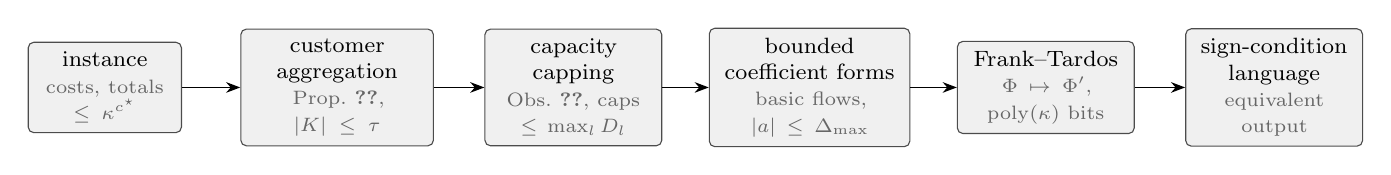
\begin{tikzpicture}[
      >={Stealth[length=1.8mm]},
      res/.style={draw=black!70,line width=0.4pt,fill=black!6,
        rounded corners=2pt,align=center,inner sep=3.5pt,
        font=\footnotesize},
      flow/.style={draw=black,line width=0.5pt,->}
    ]
    \node[res,text width=1.7cm] (I) at (0,0)
      {instance\\
       \textcolor{black!60}{\scriptsize costs, totals
       $\le\kappa^{c^\star}$}};
    \node[res,text width=2.2cm] (A) at (2.95,0)
      {customer aggregation\\
       \textcolor{black!60}{\scriptsize Prop.~\ref{prop:aggregation},
       $|K|\le\tau$}};
    \node[res,text width=2.0cm] (C) at (5.95,0)
      {capacity capping\\
       \textcolor{black!60}{\scriptsize Obs.~\ref{obs:capping}, caps
       $\le\max_l D_l$}};
    \node[res,text width=2.3cm] (S) at (8.95,0)
      {bounded coefficient forms\\
       \textcolor{black!60}{\scriptsize basic flows,
       $|a|\le\Delta_{\max}$}};
    \node[res,text width=2.0cm] (F) at (11.95,0)
      {Frank--Tardos\\
       \textcolor{black!60}{\scriptsize $\Phi\mapsto\Phi'$,
       $\mathrm{poly}(\kappa)$ bits}};
    \node[res,text width=2.0cm] (L) at (14.85,0)
      {sign-condition language\\
       \textcolor{black!60}{\scriptsize equivalent output}};
    \draw[flow] (I) -- (A);
    \draw[flow] (A) -- (C);
    \draw[flow] (C) -- (S);
    \draw[flow] (S) -- (F);
    \draw[flow] (F) -- (L);
  \end{tikzpicture}%
  }
  \caption{The compression pipeline of
  Proposition~\ref{prop:ftcompress}. Aggregation and capping
  (Prop.~\ref{prop:aggregation}, Obs.~\ref{obs:capping}) bound the
  entities and the numeric entries by $\mathrm{poly}(\kappa)$, total
  unimodularity of the oracle networks of
  Proposition~\ref{prop:oracle} turns acceptance into sign conditions
  on integer forms with coefficients of magnitude at most
  $\Delta_{\max}$, and the Frank--Tardos step replaces the cost vector
  $\Phi$ by an equivalent $\Phi'$ of $\mathrm{poly}(\kappa)$ bits, so
  the bounded subclass compresses in $\kappa$.}
  \label{fig:ftpipeline}
\end{figure}


\begin{proposition}[kernel and compression under one-sided
bounds]\label{prop:ftcompress}
Fix $c^\star$ and let $\kappa=|I|+|J|+|L|+\tau$. The subclass of
$\mathrm{MP\text{-}TSCFLP}(B)$ whose opening and transport costs
$f,g,c,d$ and whose total demands $D_1,\dots,D_{|L|}$ are integers at
most $\kappa^{c^\star}$, with capacities and budget unrestricted,
admits a polynomial kernel in $\kappa$, an equivalent instance of
$\mathrm{MP\text{-}TSCFLP}(B)$ itself of $\mathrm{poly}(\kappa)$
bits. The subclass with $\max(f,g,c,d,B)\le\kappa^{c^\star}$ and
capacities and demands unrestricted admits a
polynomial compression in $\kappa$ into a fixed sign-condition
language, which is not itself a location problem. The first subclass is nontrivial.
The strongly hard slice with $|K|=|L|=1$ of Theorem~\ref{thm:numeric}
has costs in $\{0,1\}$ and a single customer whose demand, the only
product total, is $|I|\,(|J|+1)\le\kappa^{2}$, so the slice lies in the
subclass for every $c^\star\ge 2$.
\end{proposition}
The proof, given in Appendix~\ref{app:ft}, is elementary for the first
subclass. Aggregation and capping leave every datum except the budget
within $\kappa^{c^\star}$, the all-open design decides feasibility
outright, and its cost, itself polynomially bounded in $\kappa$, caps
the budget, so the output is an ordinary instance of the problem. No
such cap exists in the second subclass, whose large numbers are the
capacities and demands, and there acceptance becomes a Boolean
combination of sign conditions on integer linear forms with
coefficients that total unimodularity bounds by a fixed power of
$\kappa$, which the
Frank--Tardos theorem compresses to
$\mathrm{poly}(\kappa)$ bits preserving every sign at once.

The matching negative result completes the account. Two cross-compositions
of \textsc{Set Cover} show that, unless
$\NP\subseteq\mathrm{coNP}/\mathrm{poly}$, the parameter of the dichotomy
admits no polynomial kernel, and
the same construction reaches the augmented parameters and the unary
encoding.

\begin{theorem}[no polynomial kernel]\label{thm:nokernel}
Unless $\NP\subseteq\mathrm{coNP}/\mathrm{poly}$,
$\mathrm{MP\text{-}TSCFLP}(B)$ parameterized by $|I|+|J|$ admits no
polynomial compression, and in particular no polynomial kernel, already on
the subclass $|I|=|L|=1$ and even with unary data. The exclusion transfers
to the parameters $|I|+|J|+|L|$ and $|I|+|J|+|K|$, to the cardinality
version $\mathrm{MP\text{-}TSCFLP}(B,k)$, and to the subclass $|K|=1$.
\end{theorem}
\begin{proof}
We give an OR-cross-composition of \textsc{Set Cover} \citep{Karp1972}
into $\mathrm{MP\text{-}TSCFLP}(B)$ parameterized by $|I|+|J|$, which by
the framework of \citet{BodlaenderJansenKratsch2014} rules out a
polynomial compression unless $\NP\subseteq\mathrm{coNP}/\mathrm{poly}$.
The framework asks for a polynomial equivalence relation, and we take
the relation $R$ that declares two well-formed instances equivalent when
they agree on the universe size $|U|$, the family size $m$ and the
target $t$, with $|U|\ge 1$ and $1\le t\le m$. Four further classes are
reserved, one for the malformed inputs, one for the well-formed
instances with empty universe, one for those with nonempty universe and
$t=0$, and one for those with nonempty universe and $t>m$.
Each instance falling in one of these four classes is decided
individually in polynomial time, a malformed input being rejected by
the syntactic check that recognizes it, an empty universe being covered
by the empty subfamily, a target of zero over a nonempty universe
admitting no cover, and a target above $m$ admitting one exactly when
the whole family covers the universe. On inputs from those classes the composition
therefore answers the OR of those individual answers, emitting a fixed
yes- or no-instance realizing it. Deciding $R$ compares three numbers, and
the triple $(|U|,m,t)$ takes at most cubically many values in the total
encoding length of the input list, so
$R$ is a polynomial equivalence relation in the sense of the framework.

Take now $T$ \textsc{Set Cover} instances $X_1,\dots,X_T$ from one
nontrivial class, sharing $|U|\ge 1$, $m$ and $t$ with $1\le t\le m$,
and assume
$T=2^{s}$ with $s=\lceil\log T\rceil$ by duplicating instances,
duplicating once more when $T=1$ so that $s\ge 1$. Identify the copies
with the strings of $\{0,1\}^{s}$ and write $c_a$ for the $a$th bit of
the copy index $c$. The budget is $B=s(t+1)+t$, the amplifier is
$Q=B+1$, and the customers comprise $T|U|$ copy customers and $s$ guard
customers, one guard per index bit, each of demand $Q$, so a customer
forced onto arcs of unit cost pays at least $Q>B$ even under divisible
service, exactly the accounting of Theorem~\ref{thm:cover}. The
composed instance has a single product and a single factory of opening
cost zero, capacity $(T|U|+s)\,Q$ equal to the total demand, and zero
first-stage costs, so the whole construction lives in the depot layer
and the second-stage matrix, and $|I|=|L|=1$ throughout.

\emph{Depots.} Use $m$ set-depots $D_1,\dots,D_m$ of opening cost $1$,
shared across all copies, and $s$ pairs of selector depots
$(P_a^{0},P_a^{1})$, one pair per index bit, each of opening cost $t+1$.
Every depot has capacity equal to the total demand. Sharing the
set-depots is sound, and no instance is merged, because the
copy-specific set membership is carried not by the depots but by the
cost matrix to the copy-specific customers introduced next. Opening
$P_a^{b}$ reads bit $a$ of the selected index as $b$. A guard customer
per pair reaches either selector of its own pair at cost $0$ and every
other depot at cost $1$. A pair with neither selector open therefore
leaves its guard on unit-cost arcs at a cost of at least $Q$, so at
least one selector per pair must open. The opening charges cap the
number of open selectors, since $s+1$ open selectors already cost
$(s+1)(t+1)=s(t+1)+t+1=B+1>B$, so
jointly with the guards a within-budget design opens exactly one
selector per pair, fixing a single index $\iota\in\{0,1\}^{s}$. Because
all routing costs are nonnegative, the selector charges leave for the
set-depot openings a residual budget of exactly $B-s(t+1)=t$.

\emph{Customers.} For every copy $c$ and element $u\in U$ create a
customer $(c,u)$ with demand $Q$. The cost from set-depot $D_j$ to
$(c,u)$ is $0$ when $u$ belongs to the $j$th set of copy $c$ and $1$
otherwise, so the whole of copy $c$'s instance lives in these costs. The
cost from selector $P_a^{b}$ to $(c,u)$ is $0$ when $c_a\ne b$, and $1$
otherwise.

\emph{Correctness.} Fix the selected index $\iota$. A copy $c\ne\iota$
differs from $\iota$ in some bit $a$, so the open selector
$P_a^{\iota_a}$ serves all of copy $c$ for free, and the non-selected
copies cost nothing beyond the selectors already open. The copy $\iota$
agrees with the pattern on every bit, so every selector arc into its
customers costs one, and each $(\iota,u)$, carrying demand $Q$, must be
served through a set-depot whose set in copy $\iota$ contains $u$, since
any other service costs at least $Q>B$. Each open set-depot costs $1$
against the residual budget $t$, so at most $t$ set-depots are open.
Every element $u$ therefore has an open set-depot whose set in copy
$\iota$ contains it, and those sets form a cover of
$X_\iota$ of size at most $t$. Conversely, if some $X_\iota$ has a cover
of size at most $t$, open the factory, the selector pattern of $\iota$ and
that cover. Every depot has capacity equal to the total demand, so with
the free factory and these depots open (F1) and (F2) hold and the design
is feasible by Proposition~\ref{prop:feas}. Completeness of the two
stages then lets every customer draw its demand through a zero-cost
depot. The guards use the open selector of their own pair, the customers
of a copy $c\ne\iota$ use the open selector $P_a^{\iota_a}$ at a bit $a$
where $c$ disagrees with $\iota$, as in the forward direction, and the
customers of copy $\iota$ use the depots of the cover, so the routing
cost is zero and the total cost is the fixed charge
$s(t+1)+|C|\le s(t+1)+t=B$. A within-budget design therefore exists if and
only if the OR of the $T$ instances is a yes-instance.

\emph{Parameter and robustness.} The depots number $m+2s$ and the
factories one, so $|I|+|J|=O(m+\log T)$, polynomially bounded in the
largest input and in $\log T$ exactly as the framework requires. The
construction writes $O((T|U|+s)(m+2s))$ cost entries and numbers of
$O(\log(T|U|m))$ bits, so it runs in time polynomial in
$\sum_c\lvert X_c\rvert$, which is the framework's time bound. The
largest numbers are the capacities, equal to the total demand
$(T|U|+s)\,Q$. Here $Q=B+1=s(t+1)+t+1\le(s+1)(m+1)=O(m\log T)$ since
$t\le m$, and $s\le T\le T|U|$ since $|U|\ge 1$, so the total demand is
$O(T\,|U|\,m\log T)$, hence polynomial in the output size,
so the composition is robust to a unary encoding, and the single product
places it in the subclass $|I|=|L|=1$ while inflating $|K|$.

\emph{Transfer to $|K|=1$.} The dual construction keeps one depot and one
customer and moves the composition to the factory and product sides,
mirroring the primal exactly as Corollary~\ref{cor:mirror} mirrors
Theorem~\ref{thm:products}. Introduce a product $(c,u)$ of demand $Q$ for every
copy $c$ and element $u$. Introduce $m$ shared set-factories
$F_1,\dots,F_m$ of opening cost $1$, whose first-stage cost to product
$(c,u)$ is $0$ when $u$ lies in the $i$th set of copy $c$ and $1$
otherwise, together with $s$ pairs of selector factories of opening cost $t+1$,
whose cost to $(c,u)$ is $0$ when $c_a\ne b$ for the pair's bit $a$ and
read value $b$, and $1$ otherwise. Add a guard product per pair, of
demand $Q$, free through either selector factory of its pair and costing
$1$ elsewhere. The budget is again $B=s(t+1)+t$ with amplifier $Q=B+1$.
The single depot and the single customer are free, the
customer demands $Q$ units of every product, and all second-stage costs
vanish. Every factory and the depot hold, in each product separately,
capacity equal to the total demand, so
feasibility reads through (F1) and (F2) as before, and since the second
stage carries zero cost the entire penalty sits on the first stage. The
paragraphs on depots and correctness of the primal now apply verbatim under
the substitution of set-factory for set-depot, selector factory for
selector depot, product $(c,u)$ for customer $(c,u)$, guard product for
guard customer, and first-stage cost for second-stage cost, with (F1),
(F2) and the budget arithmetic unchanged. In the transferred
construction the single depot receives every product through the first
stage and forwards it to the single customer, so constraint \eqref{eq:C2}
reads, for each product, first-stage inflow at least second-stage
outflow, and the routing that serves each product through its designated
factory satisfies it with equality. The orientation of the balance
constraint is therefore respected and the budget arithmetic is
unchanged. A within-budget design
therefore selects one index $\iota$ and covers copy $\iota$'s products
with at most $t$ set-factories, and conversely a cover of size at most
$t$ yields a design of cost at most $B$. This
keeps $|K|=1$ while inflating $|L|$, with $|I|+|J|=(m+2s)+1=O(m+\log T)$
and all numbers polynomial in the output, so it excludes a polynomial
kernel on the subclass $|K|=1$ too.

Finally, the augmented parameters
match the two compositions as follows. Adding $|L|$ leaves
$|I|+|J|+|L|$ polynomially bounded in the primal composition, where
$|L|=1$, and adding $|K|$ leaves $|I|+|J|+|K|$ polynomially bounded in
the dual composition, where $|K|=1$, so each augmented parameter
inherits the exclusion from its composition. Appending the cardinality
bound $k=1+s+t$ is likewise redundant. The total demand is positive, so
(F1) forces the single factory of the primal open and (F2) forces the
single depot of the dual open, and every within-budget design opens that
forced facility, exactly one selector per pair and at most $t$
set-facilities, hence at most $1+s+t=k$ facilities in all. The witness
of the converse direction opens $1+s+|C|\le 1+s+t=k$ of them, so the
bound thins the set of witnesses and breaks
neither direction.
\end{proof}

Fixed-parameter tractability in $|I|+|J|$ still yields an exponential
kernel, by the standard equivalence between fixed-parameter
tractability and kernelization \citep[e.g.][]{Cygan2015}, since on
instances larger than a threshold depending on the parameter the \FPT\
algorithm runs in polynomial time and a trivial equivalent instance can
be output, while below the threshold the instance is its own kernel. What
Theorem~\ref{thm:nokernel} rules out is only the polynomial one, and
whether a polynomial kernel exists for the full parameter
$|I|+|J|+|K|+|L|$ with general numbers, where the yes-certificate
comparison becomes genuinely bilinear, is left open.

\subsection{Width parameters}\label{sec:width}

A reader versed in algorithmic meta-theorems might hope to route the
tractable side through graph width, and this last remark closes that door
for the representation we analyse.
The natural incidence graph carries no useful width, and over that
representation the obstruction
is arithmetic rather than structural.

\begin{observation}[width is uninformative]\label{obs:cliquewidth}
We first fix the graph the claim is about.
For every instance the layered incidence graph on $I\cup J\cup K$ is the
complete bipartite graph $K_{J,\,I\cup K}$, since
$K_{I,J}\cup K_{J,K}=K_{J,\,I\cup K}$. Its clique-width is at most $2$,
witnessed by the expression that introduces every vertex of $J$ with
label $1$, introduces every vertex of $I\cup K$ with label $2$, and
performs a single join between the two labels.

Its treewidth
\citep{RobertsonSeymour1986} equals
$\min(|J|,|I|+|K|)$ once both sides are nonempty, and is therefore
unbounded over the class. Indeed, for $K_{m',n'}$ with
$1\le m'\le n'$, the bags formed by the smaller side together with one
vertex of the larger side, one bag per such vertex and arranged along a
path, give a decomposition of width $m'$. The matching lower bound
follows by contracting a matching of size $m'-1$ between the two sides.
The contracted
vertices become pairwise adjacent, and the remaining vertex of the
smaller side and any remaining vertex of the larger side are adjacent to
all of them and to each other, so $K_{m',n'}$ has a $K_{m'+1}$ minor,
and since $K_{m'+1}$ has treewidth $m'$ and treewidth never increases
under minors \citep{RobertsonSeymour1986}, the treewidth is exactly
$m'=\min(m',n')$.

The logical consequence closes the observation.
The treewidth-one star slice with $|J|=1$ is already strongly
\NP-hard, by Theorem~\ref{thm:products} (which fixes $|J|=|K|=1$). Were
the problem expressible in the
$\mathrm{MSO}_1$ optimization logic over the unweighted incidence graph
used here, the clique-width meta-theorem
\citep{CourcelleMakowskyRotics2000} together with the bound of at most
two would force a polynomial algorithm on the whole class,
contradicting strong \NP-hardness unless $\Ppoly=\NP$, so that route is
closed. The capacity and demand constraints compare sums of numbers,
which that logic over that graph cannot express, and over the
representation used here the obstruction is therefore arithmetic rather
than structural. This persists even when every capacity, demand and
cost lies in $\{0,1,m+1\}$ and the budget is at most $m$, where $m$ is
the size of the set family in the construction of
Theorem~\ref{thm:products}. Richer relational structures, weighted or
counting logics, or representations carrying products and constraints
as objects are not addressed by this observation, and their width
status simply remains open.
\end{observation}

The results of Sections~\ref{sec:complexity} and~\ref{sec:algorithms}
assemble into a single map, and Table~\ref{tab:landscape} records it.
Figure~\ref{fig:resultsmap} shows which result feeds which before the
table lists them row by row. Each
row names a parameter or a structural restriction, states the encoding
under which the entry holds, gives the status, and traces it to the
theorem that establishes it. The rows descend from the polynomial base
through the coverage layer, the size-parameter dichotomy, the parameter
$k$ and the numeric layer to the kernelization and width entries. The
table and the figure carry the detail row by row.

% Requires: \usetikzlibrary{positioning,arrows.meta}
\begin{figure}[H]
  \centering
  \resizebox{0.99\textwidth}{!}{%
  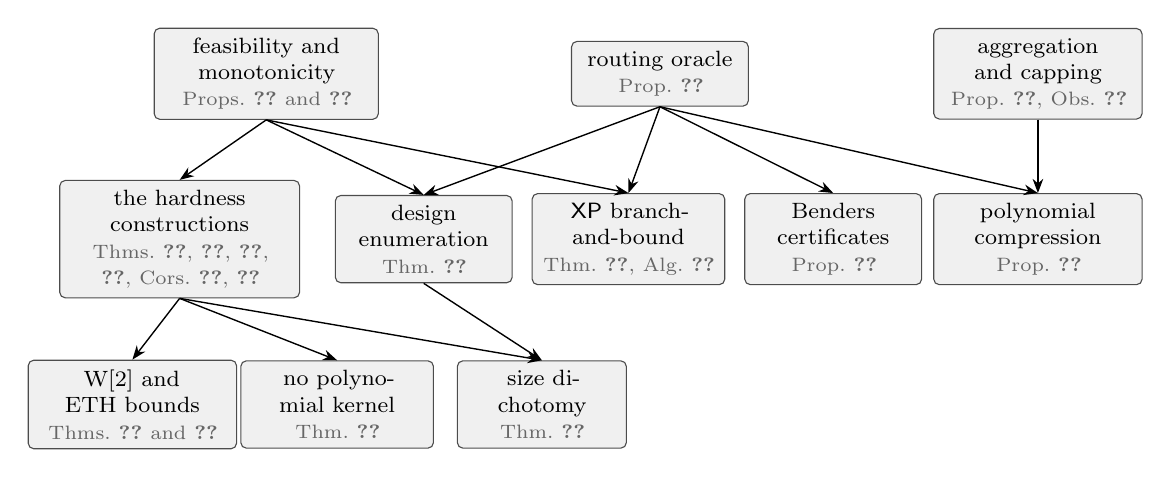
\begin{tikzpicture}[
      >={Stealth[length=1.8mm]},
      res/.style={draw=black!70,line width=0.4pt,fill=black!6,
        rounded corners=2pt,align=center,inner sep=3.5pt,
        font=\footnotesize},
      dep/.style={draw=black,line width=0.5pt,->}
    ]
    % row 1: the structural toolkit and the two reduction rules
    \node[res,text width=2.6cm] (FM) at (2.6,0)
      {feasibility and monotonicity\\
       \textcolor{black!60}{\scriptsize Props.~\ref{prop:feas}
       and~\ref{prop:mono}}};
    \node[res,text width=2.0cm] (OR) at (7.6,0)
      {routing oracle\\
       \textcolor{black!60}{\scriptsize Prop.~\ref{prop:oracle}}};
    \node[res,text width=2.4cm] (AGG) at (12.4,0)
      {aggregation and capping\\
       \textcolor{black!60}{\scriptsize Prop.~\ref{prop:aggregation},
       Obs.~\ref{obs:capping}}};
    % row 2: constructions, algorithms, certificates, compression
    \node[res,text width=2.8cm] (CC) at (1.5,-2.1)
      {the hardness constructions\\
       \textcolor{black!60}{\scriptsize Thms.~\ref{thm:cover},
       \ref{thm:products}, \ref{thm:partition}, \ref{thm:numeric},
       Cors.~\ref{cor:mirror}, \ref{cor:partitionmirror}}};
    \node[res,text width=2.0cm] (FPT) at (4.6,-2.1)
      {design enumeration\\
       \textcolor{black!60}{\scriptsize Thm.~\ref{thm:fpt}}};
    \node[res,text width=2.2cm] (XP) at (7.2,-2.1)
      {\XP\ branch-and-bound\\
       \textcolor{black!60}{\scriptsize Thm.~\ref{thm:xp},
       Alg.~\ref{alg:xpbb}}};
    \node[res,text width=2.0cm] (BC) at (9.8,-2.1)
      {Benders certificates\\
       \textcolor{black!60}{\scriptsize Prop.~\ref{prop:duals}}};
    \node[res,text width=2.4cm] (CP) at (12.4,-2.1)
      {polynomial compression\\
       \textcolor{black!60}{\scriptsize Prop.~\ref{prop:ftcompress}}};
    % row 3: the classification
    \node[res,text width=2.4cm] (W2) at (0.9,-4.2)
      {$\mathrm{W}[2]$ and ETH bounds\\
       \textcolor{black!60}{\scriptsize Thms.~\ref{thm:w2}
       and~\ref{thm:eth}}};
    \node[res,text width=2.2cm] (NK) at (3.5,-4.2)
      {no polynomial kernel\\
       \textcolor{black!60}{\scriptsize Thm.~\ref{thm:nokernel}}};
    \node[res,text width=1.9cm] (DI) at (6.1,-4.2)
      {size dichotomy\\
       \textcolor{black!60}{\scriptsize Thm.~\ref{thm:dichotomy}}};
    % dependencies
    \draw[dep] (FM.south) -- (CC.north);
    \draw[dep] (FM.south) -- (FPT.north);
    \draw[dep] (FM.south) -- (XP.north);
    \draw[dep] (OR.south) -- (FPT.north);
    \draw[dep] (OR.south) -- (XP.north);
    \draw[dep] (OR.south) -- (BC.north);
    \draw[dep] (OR.south) -- (CP.north);
    \draw[dep] (AGG.south) -- (CP.north);
    \draw[dep] (CC.south) -- (W2.north);
    \draw[dep] (CC.south) -- (NK.north);
    \draw[dep] (CC.south) -- (DI.north);
    \draw[dep] (FPT.south) -- (DI.north);
  \end{tikzpicture}%
  }
  \caption{The results of the paper as a diagram, each box naming its
  numbered statements. A solid arrow points from a result to one whose
  proof uses it, and no other relation is drawn. The structural layer
  feeds every branch, the hardness constructions carry the whole
  negative side, from the $\mathrm{W}[2]$ and ETH bounds
  (Theorems~\ref{thm:w2} and~\ref{thm:eth}) through the kernel
  exclusion (Theorem~\ref{thm:nokernel}) to the negative half of the
  dichotomy (Theorem~\ref{thm:dichotomy}), and the oracle feeds the
  algorithms, the cuts and the compression
  (Prop.~\ref{prop:ftcompress}).}
  \label{fig:resultsmap}
\end{figure}


\begingroup
\footnotesize
\setlength{\tabcolsep}{4pt}
\begin{longtable}{p{4.2cm}p{1.7cm}p{3.6cm}p{2.1cm}}
\caption{The parameterized complexity landscape of MP-TSCFLP. Each row
is a parameterization, a restriction, or a preprocessing guarantee, and
hard rows either name a witness slice or cite the witnessing
construction in their source cell. Sources refer to results of
Sections~\ref{sec:complexity} and~\ref{sec:algorithms}.}
\label{tab:landscape}\\
\toprule
Parameter / restriction & Encoding & Status & Source \\
\midrule
\endfirsthead
\multicolumn{4}{l}{\footnotesize\emph{Table~\ref{tab:landscape} (continued)}}\\
\toprule
Parameter / restriction & Encoding & Status & Source \\
\midrule
\endhead
\midrule
\multicolumn{4}{r}{\footnotesize\emph{continued on the next page}}\\
\endfoot
\bottomrule
\endlastfoot
\multicolumn{4}{l}{\emph{Polynomial base}}\\
$f\equiv 0$ and $g\equiv 0$ & both & \Ppoly & Prop.~\ref{prop:fzero}\\
$|I|=|J|=1$ & both & \Ppoly & Prop.~\ref{prop:onebyone}\\
\midrule
\multicolumn{4}{l}{\emph{Coverage layer}}\\
classical, no parameter, witness slice $|I|=|L|=1$ & both, unary-robust
& strongly \NP-hard &
Thm.~\ref{thm:cover}\\
approximation, witness $|I|=|L|=1$ & both, unary-robust & no
$\max\{1,(1-\varepsilon)\ln|K|\}$ factor unless $\Ppoly=\NP$ &
Cor.~\ref{cor:coverinapprox}\\
$|K|=1$, products carry the universe, witness slices $|J|=1$ and
$|I|=1$ & both, unary-robust & strongly \NP-hard &
Thm.~\ref{thm:products}, Cor.~\ref{cor:mirror}\\
\midrule
\multicolumn{4}{l}{\emph{Size-parameter dichotomy (under
$\Ppoly\neq\NP$, \FPT\ iff $\{|I|,|J|\}\subseteq P$)}}\\
$P\supseteq\{|I|,|J|\}$ (4 sets) & both & \FPT,
$2^{|I|+|J|}\,\mathrm{poly}(N)$ & Thm.~\ref{thm:fpt}\\
$\emptyset$, $\{|I|\}$, $\{|J|\}$, $\{|K|\}$, $\{|L|\}$,
$\{|I|,|K|\}$, $\{|I|,|L|\}$, $\{|J|,|K|\}$, $\{|K|,|L|\}$ & both &
para-\NP-hard, strong slice & Thm.~\ref{thm:dichotomy},
Cor.~\ref{cor:parak}, Cor.~\ref{cor:unary}\\
$\{|J|,|L|\}$, $\{|I|,|K|,|L|\}$, $\{|J|,|K|,|L|\}$ & binary &
para-\NP-hard, weak slice & Thm.~\ref{thm:dichotomy},
Thm.~\ref{thm:partition}, Cor.~\ref{cor:partitionmirror}\\
$\{|J|,|L|\}$, $\{|I|,|K|,|L|\}$, $\{|J|,|K|,|L|\}$ & unary & open &
Cor.~\ref{cor:unary}\\
\midrule
\multicolumn{4}{l}{\emph{The parameter $k$}}\\
$k$, lower bound, already at $|I|=|L|=1$, also budget $B$ alone and
depot count $k_z$ & both & $\mathrm W[2]$-hard & Thm.~\ref{thm:w2}\\
$k$, membership & both & in $\mathrm W[\mathrm P]\cap\XP$ &
Rem.~\ref{rem:w2mem}, Thm.~\ref{thm:xp}\\
$k$, algorithm & both & \XP, $O(n^{k}\,T_{\mathrm{orac}})$ &
Thm.~\ref{thm:xp}\\
$k$, fine bound & both & no $f(k)N^{o(k)}$ under ETH &
Thm.~\ref{thm:eth}\\
a priori bound $k^\ast$ & both & exact lower bound on the opening
count, $O(m\log m)$ & Lem.~\ref{lem:cover}\\
\midrule
\multicolumn{4}{l}{\emph{Numeric layer}}\\
$|K|=|L|=1$, general transport & both, unary-robust & strongly \NP-hard &
Thm.~\ref{thm:numeric}\\
$|K|=|L|=1$, separable $c_{ij}=\gamma_i+\delta_j$ & binary &
pseudo-polynomial & Thm.~\ref{thm:separable}\\
$|J|=|L|=1$ ($|I|,|K|$ free), hard already at $|K|=1$ & binary &
weakly \NP-hard, pseudo-polynomial &
Thm.~\ref{thm:partition}, Obs.~\ref{obs:quadrant},
Thm.~\ref{thm:separable}\\
$|I|=|K|=|L|=1$, depot mirror & binary & weakly \NP-hard,
pseudo-polynomial & Cor.~\ref{cor:partitionmirror}\\
\midrule
\multicolumn{4}{l}{\emph{Kernelization and width}}\\
customer aggregation, identical columns & both & exact,
$|K|\le\tau$ & Prop.~\ref{prop:aggregation}\\
capping $b_{il},p_{jl}\le D_l$ & both & exact & Obs.~\ref{obs:capping}\\
kernel in $|I|+|J|$ & both & exponential (standard equivalence) &
Thm.~\ref{thm:fpt}\\
polynomial kernel in $|I|+|J|$ ($+|K|$, $+|L|$, and the cardinality
version), already at $|I|=|L|=1$ and at $|K|=1$ & both, unary-robust &
none unless $\NP\subseteq\mathrm{coNP}/\mathrm{poly}$ &
Thm.~\ref{thm:nokernel}\\
compression in $\kappa=|I|+|J|+|L|+\tau$, costs and total demands
bounded by $\kappa^{c^\star}$ (capacities free), likewise costs and
$B$ bounded (capacities and demands free) & binary &
polynomial compression & Prop.~\ref{prop:ftcompress}\\
polynomial kernel in $|I|+|J|+|K|+|L|$, general numbers & binary & open &
Sec.~\ref{sec:kernel}\\
$\mathrm{cwd}(G_{\mathrm{inc}})$ & --- & $\le 2$, uninformative &
Obs.~\ref{obs:cliquewidth}\\
$\mathrm{tw}(G_{\mathrm{inc}})$ & --- & unbounded, slice $\mathrm{tw}=1$
strongly hard & Obs.~\ref{obs:cliquewidth},
Thm.~\ref{thm:products}\\
\end{longtable}
\endgroup

\section{Computational study}
\label{sec:experiments}

The experiments pursue three questions. (Q1) Is the enumeration algorithm of
Theorem~\ref{thm:xp} practical in its predicted regime, and where does that
regime end. (Q2) How does it compare with the standard mixed-integer approach.
(Q3) Does the covering bound $k^\ast$ track instance difficulty beyond the
algorithm that motivated it, and through which mechanism. The remainder of the section is organised so that
the reader can locate each answer directly. Section~\ref{sec:exp-setup}
describes the codes, the instance families and the machines.
Section~\ref{sec:exp-q1} answers Q1 on the family whose covering bound is
controlled by construction, Section~\ref{sec:exp-q2} addresses Q2 against
the integer programming baseline, and Section~\ref{sec:exp-q3} addresses
Q3 by
confronting $k^\ast$ with the effort of a solver that makes no use of it.

\subsection{Setup}
\label{sec:exp-setup}

The study compares three exact codes. The first (\textsc{Xp}) is a C++20
implementation of Algorithm~\ref{alg:xpbb}, with the covering pruning, the
admissible cost bound and the dominance rule of Section~\ref{sec:algorithms},
and a deadline-aware enumerator. The baseline (\textsc{Mip}) is the compact
model \eqref{eq:obj}--\eqref{eq:dom} solved by Gurobi. A third code
(\textsc{Bd}) solves the same model by a branch-and-Benders-cut in which the
per-product transportation subproblems are separated by the disaggregated cuts
of Proposition~\ref{prop:duals}. All three read the same instance files.
The \textsc{Xp} implementation was cross-validated against an independent
brute-force enumeration of all designs with an exact per-product min-cost-flow
oracle, matching it on $180$ small seeded instances and on $1{,}381$ exact
comparisons of optimal value, feasibility and covering bound across a full sweep
of the cardinality, with no disagreement. The verification battery in the
accompanying code performs on the order of nine hundred thousand
individual checks, spanning design enumerations, closed-form comparisons
and LP cross-checks, with no failure. More than $560{,}000$ of the
checks are exhaustive design enumerations validating the numeric-layer
constructions alone, roughly ten thousand are equivalence
verifications, two hundred are independent LP cross-checks, $1{,}381$
are cross-solver comparisons, and the remainder are per-construction
parameter sweeps.

The study uses two instance families, the first with a main grid and a
boundary extension, the second the benchmark. The first is a family with controlled
covering bound, built by a deterministic generator seeded by the parameter
tuple, in which, on each side, one facility fewer than the per-side target
receives capacities that jointly fall one unit short of the binding
product's demand, a choice that pins the per-side covering count to the
target. The main
grid has target per-side count in $\{2,3,4,5,6\}$, so $k^\ast\in\{4,6,8,10,12\}$,
factory and depot counts in $\{20,40\}$, customers in $\{50,100\}$, products in
$\{5,10\}$ and five seeds, for $400$ instances, and a boundary extension on
smaller graphs, with per-side target in $\{2,4,6,8\}$ so
$k^\ast\in\{4,8,12,16\}$ and $n=|I|+|J|$ over $\{20,24,28,30,40\}$, probes where
the regime ends, adding $60$ instances for $460$ runs in all. The
generator records the recomputed bound alongside each instance, and on
all $460$ instances the recomputed $k^\ast$ equals the target exactly.
The second family is the classical
benchmark of \citet{MauriEtAl2021}, its $100$ instances split into four size
groups $|I|$-$|J|$-$|K|$ of $50$-$100$-$200$ and $100$-$200$-$400$ with
$|L|\in\{5,10\}$, for which no optimal value was proven in \citet{MauriEtAl2021} nor, to
our knowledge, since. On these instances the customer-aggregation rule of
Proposition~\ref{prop:aggregation} never applies, since in every one of
the $100$ instances no two customers share their full cost column and
hence $\tau=|K|$. Capacity capping leaves every benchmark capacity
unchanged, since no capacity exceeds its product's total demand,
customer aggregation never applies as just noted, and the covering
bound is thus the only signal the paper's toolkit produces on these
instances. One by-product of
parsing them is used repeatedly
below and is recorded here. Every
datum is integral, so the optimal value is integral by
Proposition~\ref{prop:oracle}, and a solver that reports optimality with
an absolute gap below one therefore determines the exact optimum,
subject to the floating-point tolerances under which the solver
certifies its bound, a caveat Section~\ref{sec:exp-q2} makes explicit
for the three closed runs. The
terminal gap of a run is the relative optimality gap the solver reports
when it stops, the difference between incumbent and bound divided by the
incumbent, quoted in percent throughout.

The enumeration runs were executed under a fixed $60$~s limit. The
\textsc{Xp} binary is single-threaded C++20, compiled with g++~13.3.0 at
optimisation level O2, and ran on a Linux virtual machine with an Intel
Xeon processor at $2.1$~GHz.
The integer programming runs use Gurobi $13.0.2$ on an Intel Core i9-14900HX
with $24$ cores under Windows, with the controlled family limited to $600$~s
and the benchmark to $3{,}600$~s. Gurobi ran with default tolerances,
automatic thread count and a fixed seed recorded with every run, and on
each run the harness recomputed the incumbent's cost independently from
its flows, with agreement on all $900$ runs. The enumeration and the
integer programming codes ran on different machines, so times are
compared only within a code and never across codes, and the
solved-versus-censored contrasts that the section draws are insensitive
to the hardware difference. The asymmetry of the limits favours the
baseline by
design. The enumeration limit maps where that algorithm stops being fast, the
larger Gurobi budget gives the baseline its best chance of producing
reference optima, and a censored run enters a speed comparison only
through the lower bound its limit certifies. The time of a censored run
is recorded at its limit. Every completed enumeration run is
deterministic, and each instance was run once. The software archive with
the codes, the instance generator and manifests, the raw result files and
one verification script per hardness construction accompanies the
submission as supplementary material and is released at
\url{https://github.com/pehgonzalez/mp-tscflp-parameterized}.

\subsection{The regime of the enumeration algorithm (Q1)}
\label{sec:exp-q1}

The controlled family was built to probe the boundary that
Theorem~\ref{thm:xp} predicts, and the outcome is unambiguous. The main grid, whose
graphs all have $n=|I|+|J|\ge 40$, lies entirely outside the $60$~s regime, so
all $400$ instances are censored. This is the result rather than a failure of
protocol. At $n\ge 40$ the search processes a median of roughly
$2{,}700$ nodes before the limit, while a completed search at $n=24$
already needs a median of roughly $50{,}000$, and the cost of each node
grows with $|I|$, $|J|$, $|K|$ and $|L|$ through the oracle. The raw
per-run records in the archive carry node, pruning and oracle
counters. The boundary extension locates the frontier, and
Table~\ref{tab:q1boundary} reports it in full. Each boundary cell holds
three seeded runs and the medians are taken over solved runs only, so the
times are indicative and the visible values at $n=24$ are biased downward
by that conditioning. At $n=20$ every instance
solves, at $n=24$ seven of twelve solve, and from $n=28$ upward none solves
within the limit, so the boundary observed for this implementation
under this protocol, in plain optimisation mode,
sits at $n\approx 24$. The same table shows the covering-bound effect at
fixed size, with the median time at $n=20$ falling from $13.7$~s at
$k^\ast=4$ to $0.6$~s at $k^\ast=16$. Figure~\ref{fig:q1} shows both
readings graphically, the boundary in panel (a) and the covering-bound
effect in panel (b).

\begin{table}[H]
\centering
\caption{The boundary extension of Q1 under the $60$~s limit. Each cell
reports solved over attempted instances at the given $n=|I|+|J|$ and
covering-bound target $k^\ast$, with the median time in seconds of the
solved runs in parentheses. Solved runs vanish beyond $n=24$, and in the
solvable rows a larger bound solves faster. Starred cells have fewer
than three solved runs and their medians are individual observations.}
\label{tab:q1boundary}
\begin{tabular}{lcccc}
\hline
$n$ & $k^\ast=4$ & $k^\ast=8$ & $k^\ast=12$ & $k^\ast=16$ \\
\hline
$20$ & 3/3 (13.7) & 3/3 (4.0) & 3/3 (2.3) & 3/3 (0.6) \\
$24$ & 1/3 (58.7)$^{\star}$ & 1/3 (57.2)$^{\star}$ & 2/3 (36.2)$^{\star}$ & 3/3 (15.0) \\
$28$ & 0/3 & 0/3 & 0/3 & 0/3 \\
$30$ & 0/3 & 0/3 & 0/3 & 0/3 \\
$40$ & 0/3 & 0/3 & 0/3 & 0/3 \\
\hline
\end{tabular}
\end{table}


\begin{figure}[H]
\centering
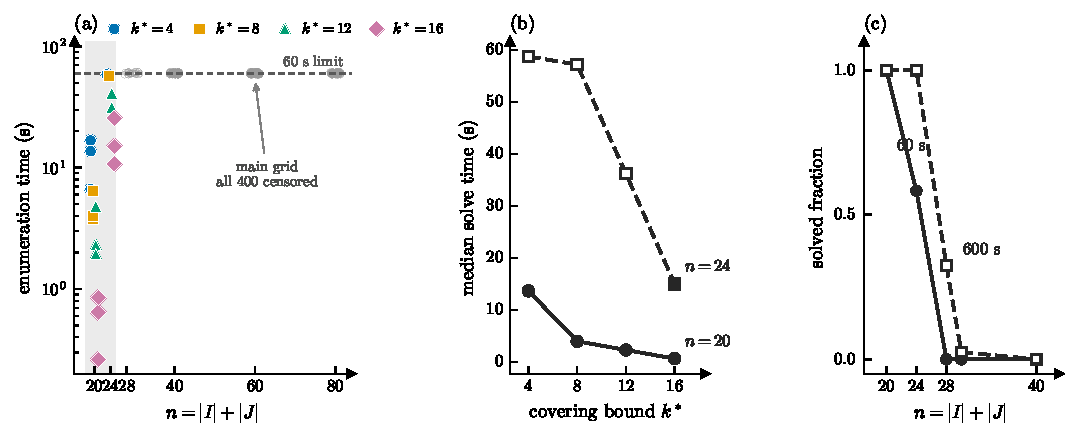
\includegraphics[width=\textwidth]{fig_q1_regime.pdf}
\caption{The enumeration algorithm on the controlled family, all $460$ runs
under the $60$~s limit. Panel (a) plots time against $n=|I|+|J|$. Solved runs
are filled and coloured by the covering bound $k^\ast$, and they occur only in
the shaded band up to $n\approx 24$. Every run beyond it is censored, shown as
grey open circles on the limit line, including the whole $400$-instance main
grid, which lies at $n\ge 40$. Panel (b) gives the median solve time against $k^\ast$ at
$n=20$ and $n=24$, where instances with a larger bound solve faster,
with medians taken over solved runs only. Open markers in panel (b) are
medians over fewer than three solved runs. Lower is better in both
panels, and the censored band beyond $n\approx 24$ is the observed
border of the regime that Theorem~\ref{thm:xp} delimits.}
\label{fig:q1}
\end{figure}

Within the solvable range the covering bound acts in a direction that
requires explanation. Time and node counts decrease as $k^\ast$ grows,
and the solved count at $n=24$ in Table~\ref{tab:q1boundary} rises from
one in three at $k^\ast=4$ to three in three at $k^\ast=16$. The
covering pruning of Lemma~\ref{lem:cover} is the mechanism compatible
with this pattern. In plain optimisation the
cardinality never binds, so $k^\ast$ can act on the search only through
that pruning, and tight capacities let it discard subtrees
that loose capacities leave standing. The generator, however, varies
capacities to move the bound and therefore moves other instance
features with it, so an ablation isolating the pruning is left for
future work. The mirror pattern expected for the
cardinality sweep, in which the exponent $n^k$ grows with the target count, is
left for a dedicated run.

\subsection{Comparison with the mixed-integer approach (Q2)}
\label{sec:exp-q2}

Q2 places the enumeration and the integer programming codes side by
side, each under its own protocol, and the observed outcome is an
empirical result consistent with the worst-case limitation of support
enumeration rather than a consequence of it. Outside the
small-$n$ regime the weight-independent enumeration bound gives \textsc{Xp} no
way to prune below $n^{k}$, whereas the compact model carries the linear
structure a modern solver exploits, so \textsc{Mip} is expected to close quickly the very controlled-family
instances on which \textsc{Xp} exhausts its $60$~s budget. The campaign
realises that expectation, and Table~\ref{tab:q2codes} summarises it.
\textsc{Mip} closes all $400$ controlled instances with a median solving
time of $0.55$~s, among them every instance the enumeration had left
censored at $60$~s.

\begin{table}[H]
\centering
\caption{The three exact codes on the $400$-instance main grid of the
controlled family, whose graphs all have $n\ge 40$. Solved means proven
optimal within the per-code limit. The median time is over solved runs
only, in seconds. \textsc{Mip} closes every instance the enumeration
leaves censored, the empirical face of the regime border of Q1. The
enumeration ran on a different machine from the two integer programming
codes, which shared one machine, so times compare only within a code
and between \textsc{Mip} and \textsc{Bd}, and the cross-code reading
is the solved-versus-censored contrast.}
\label{tab:q2codes}
\begin{tabular}{lccc}
\hline
code & limit (s) & solved & median time (s) \\
\hline
\textsc{Xp} & $60$ & $0/400$ & -- \\
\textsc{Mip} & $600$ & $400/400$ & 0.55 \\
\textsc{Bd} & $600$ & $8/400$ & 395.57 \\
\hline
\end{tabular}
\end{table}
 The value of
Theorem~\ref{thm:xp} is thus classificatory rather than competitive, and
the observed dominance is no defeat of the algorithm but an
empirical face consistent with the same hardness the theory maps. What the exact codes
earn is not speed but proof, since by the integrality remark of
Section~\ref{sec:exp-setup} a solver that closes an instance settles a
value the benchmark of \citet{MauriEtAl2021} had left to heuristics. On
the benchmark itself the $3{,}600$~s budget proves optimality on three of
the $100$ instances, all in the smaller size group with five products,
values the original study left unproven. The three instances are
PSC1-C1-50-5, PSC4-C1-50-5 and PSC5-C1-50-5, closed at optimal values
$1{,}923{,}801$, $1{,}909{,}659$ and $1{,}895{,}151$ in $2{,}001$, $642$
and $883$ seconds. Each value lies strictly below the best solution
reported for the same instance by \citet{MauriEtAl2021}, respectively
$1{,}923{,}813$, $1{,}910{,}011$ and $1{,}896{,}699$, so the campaign
closes the three instances and improves their best-known solutions at the
same time. On these three runs the terminal bound equalled the incumbent
at the recorded precision, and we report the optima subject to the
solver's default floating-point certificates, with the incumbent costs
confirmed by the independent recomputation noted above.
The branch-and-Benders-cut \textsc{Bd} enters here not as a faster
solver, for it closes $8$ of the $400$ controlled instances within the
same budget, but as a device for cross-validation and for the structural
reading of Proposition~\ref{prop:duals}, and the codes are compared only
on optimal values they jointly certify.

\subsection{The covering bound and the root relaxation (Q3)}
\label{sec:exp-q3}

The last question asks whether $k^\ast$ tracks difficulty beyond the
algorithm that motivated it, and through which mechanism, so we
confront the covering bound with the integer
solver on the benchmark that the original study left without a single proven
optimum. The bound is available
without solving anything, computed by one sort and one prefix scan,
and it varies widely across the benchmark, as Figure~\ref{fig:q3} shows. Table~\ref{tab:q3groups} reports the campaign by
size group, the range of the bound, the median terminal gap, the proven
optima and the within-group correlations with their Holm-adjusted
$p$-values. Within every size group the
bound spreads over a factor of four or more, and this spread at fixed
size removes the most evident confounder, instance size, while other
instance features still vary within a group, so the bound may in part
proxy properties the design does not separate.

\begin{table}[H]
\centering
\caption{The benchmark campaign by size group, $3{,}600$~s per instance.
Columns give the group $|I|$-$|L|$, the instance count, the minimum,
median and maximum of the covering bound $k^\ast$, the median terminal
gap in percent, the number of proven optima, the within-group Spearman
correlation between $k^\ast$ and the terminal gap, and its
Holm-adjusted two-sided permutation $p$-value. Correlations carry
percentile bootstrap $95\%$ confidence intervals in brackets. Each
interval describes one group alone, and the within-group column is the
sharper instrument, the pooled value mixing the group effect with size.
The pooled correlation over all $100$ instances is $-0.28$,
Holm-adjusted $p=0.013$.}
\label{tab:q3groups}
\small
\setlength{\tabcolsep}{4pt}
\begin{tabular}{lcccccc}
\hline
group & $\#$ & $k^\ast$ min/med/max & gap (\%) & opt.\ &
$\rho$ [$95\%$ CI] & $p$ \\
\hline
$50$-$5$ & $25$ & $8$/$17$/$36$ & $0.4$ & $3$ & $-0.59$ [$-0.81$, $-0.22$] & $0.006$ \\
$50$-$10$ & $25$ & $8$/$17$/$35$ & $0.4$ & $0$ & $-0.39$ [$-0.69$, $+0.09$] & $0.102$ \\
$100$-$5$ & $25$ & $14$/$32$/$67$ & $1.1$ & $0$ & $-0.70$ [$-0.86$, $-0.45$] & $0.001$ \\
$100$-$10$ & $25$ & $14$/$33$/$69$ & $4.2$ & $0$ & $-0.40$ [$-0.75$, $+0.12$] & $0.102$ \\
\hline
\end{tabular}
\end{table}


\begin{figure}[H]
\centering
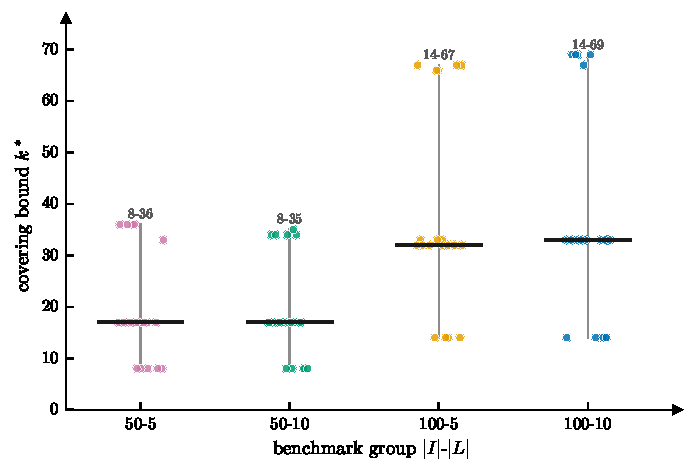
\includegraphics[width=0.8\textwidth]{fig_q3_kstar.pdf}
\caption{The covering bound $k^\ast$ across the four benchmark groups. Each
point is one instance and the bar marks the group median. The bound spreads by
a factor of more than four inside every group, varying across instances of
equal size, so its variation is not a proxy for instance size.}
\label{fig:q3}
\end{figure}

The completed campaign lets the correlation between $k^\ast$ and the
effort \textsc{Mip} spends on the $100$ benchmark instances be read
directly, with a within-group control that separates the effect of the
bound from the effect of size. Pooled over the benchmark, the covering
bound and the terminal gap are rank-correlated with Spearman
$\rho=-0.28$. Ninety-seven of the hundred runs end at the limit, so
solving time carries no usable signal on this benchmark and the analysis
reads the terminal gap alone. The terminal gap blends primal and dual
progress and depends on the objective scale and on the solver
tolerances, so it is an imperfect proxy of computational effort.
Within the four size groups the association strengthens, the four
coefficients being negative throughout and ranging from
$-0.39$ to $-0.70$ with descriptive mean $-0.52$, as the $\rho$ column
of Table~\ref{tab:q3groups}
shows. Significance was assessed by a two-sided permutation test on the
Spearman statistic. The test is Monte Carlo with $20{,}000$
permutations under a fixed seed, the $p$-value uses the add-one
convention so it cannot vanish, ties including zero gaps are handled by
mid-ranks, and every reported $p$-value is Holm-adjusted over the five
gap correlations. The pooled correlation and the two five-product
groups survive the correction, with adjusted $p$-values of $0.013$,
$0.006$ and $0.001$, while the two ten-product groups do not, and the
$p$ column of Table~\ref{tab:q3groups} reports the adjusted value of
every group. The direction is negative in all four groups, established
where the test passes and inconclusive where it does not. The bootstrap
intervals of Table~\ref{tab:q3groups} tell the same story, excluding
zero exactly in the groups that survive the correction.
Figure~\ref{fig:q3scatter} plots the hundred instances behind these
coefficients, and the negative drift is visible inside each group.
The sign is the substantive finding. A naive reading
of the bound would predict the opposite, a small $k^\ast$ meaning few
facilities to open and hence an easy instance, but on this benchmark
larger bounds go with smaller terminal gaps, the same inverse direction
the enumeration exhibits in Q1, where tight capacities give the covering
pruning its greatest effect.

The stored solver logs admit a mediation analysis that locates the
mechanism, extracted by a pinned script with no further runs. The
terminal gap on this benchmark is essentially the root relaxation gap,
the two rank-correlating between $+0.89$ and $+1.00$ within groups and
at $+0.97$ pooled. The covering bound correlates with the root gap
between $-0.42$ and $-0.73$ in every group ($-0.36$ pooled), and once
the root gap is controlled the partial rank correlation of the bound
with the terminal gap collapses, ranging from $-0.04$ to $+0.52$ across
groups with no stable sign ($+0.29$ pooled). The bound moreover
correlates positively with the explored node count in every group. The
association of the bound with solver effort is therefore mediated by
the relaxation. Tight capacities give tight root relaxations, and
within the $3{,}600$~s budget the solver rarely moves far from its root
bound. On this benchmark the covering bound annotates relaxation
tightness rather than search difficulty, its direction stable across
groups and its strength moderate within the five-product groups and
weaker pooled. We make no causal claim beyond the controlled
comparison.

\begin{figure}[H]
\centering
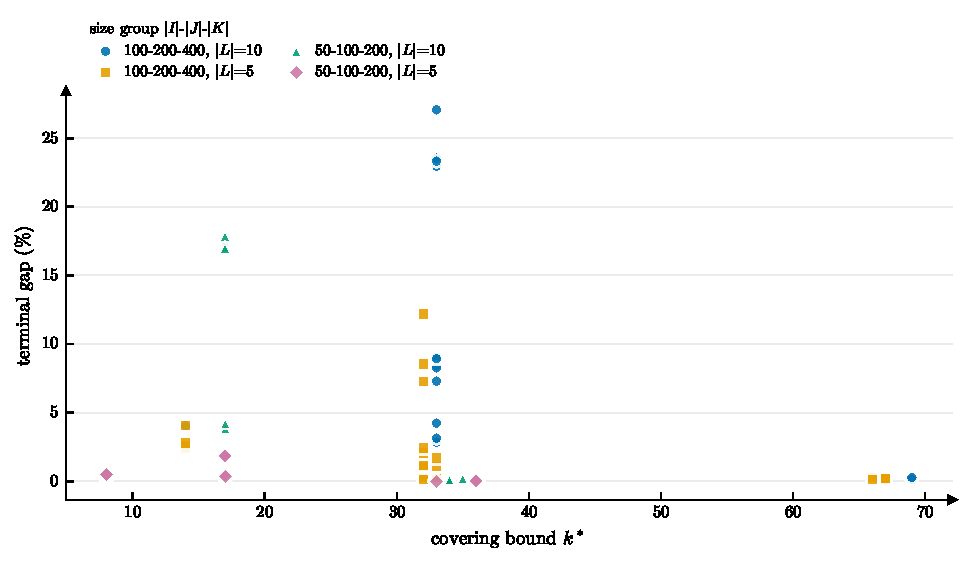
\includegraphics[width=0.85\textwidth]{fig_q3_scatter.pdf}
\caption{Terminal gap of \textsc{Mip} under the $3{,}600$~s limit
against the covering bound $k^\ast$, one marker per benchmark
instance, coloured by size group. Within every group larger bounds
accompany smaller gaps, the association Table~\ref{tab:q3groups}
quantifies. The within-group reading is what controls for instance
size.}
\label{fig:q3scatter}
\end{figure}

\section{Conclusion}\label{sec:conclusion}

We gave a parameterized account of MP-TSCFLP, and the picture that
emerges has two layers, a coverage layer, structural and strong, that
fires wherever a facility side sees a dimension discriminating it
through a $\{0,1\}$ incidence matrix, and a numeric layer, weak, that
dissolves under a unary encoding where no pair discriminates.
Table~\ref{tab:landscape} and Figure~\ref{fig:resultsmap} record the
resulting landscape entry by entry, from the size-parameter dichotomy
through the bracketing of the parameter $k$ to the kernelization and
width results, with witnesses on both sides of every border of the
binary-encoding map.

Five questions remain, and we regard them as the natural continuation of
this work. The first asks for a greedy $\ln|K|$ upper bound matching the
inapproximability of the coverage layer, the constructive half that would
close the approximability of that layer from above and below, with the
non-metric uncapacitated median problem \citep{Hochbaum1982} as the
precedent. A parameterized companion attaches to the same layer. The
reduction behind Theorem~\ref{thm:cover}, run with the enlarged
amplifier of Corollary~\ref{cor:coverinapprox}, maps the minimum cover
size onto the optimum value while shifting the parameter by one, so a
constant-factor \FPT\ approximation in $k$ for MP-TSCFLP would hand
back one for \textsc{Set Cover} parameterized by the cover size, which
is itself $\mathrm W[2]$-hard to approximate within any constant
\citep{LinRenSunWang2023}, and we conjecture that no such approximation
exists. The second concerns membership of the parameter $k$ in $\mathrm
W[2]$, since our sandwich leaves the exact class as the one open
classification of the project, and the barrier of binary arithmetic and
flow minimisation inside the verifier against weft two is of interest
beyond this model. The third would settle the unary status of $\{|J|,|L|\}$ and
of the two triples $\{|I|,|K|,|L|\}$ and $\{|J|,|K|,|L|\}$, the only gaps
of the sixteen-by-two dichotomy table, where the witnessing slices go
polynomial under unary data and no other hard slice is yet known. The
fourth is whether a polynomial kernel exists in the full parameter
$|I|+|J|+|K|+|L|$ with general numbers, the exact point where the
yes-certificate comparison turns bilinear and both weight families would
have to be reduced at once, a genuine methodological frontier of weighted
kernelization. The fifth turns to transport costs structured
beyond separability, uniform per side, metric or of low rank, fall on the
tractable or the hard side, refining the frontier over the cost classes
that appear in real data. Every hardness construction in the paper uses
transport costs without metric structure, so the map may bind
differently on distance-based data, and the fifth open problem asks
exactly that question. Progress on any one of the five would redraw a
border of the landscape assembled here.

For practice the reading is brief and concrete. The a priori bound
$k^\ast$ is computed by a sort and a prefix scan of the capacities per
product and side, and by nothing costlier,
lower-bounds the
facilities any feasible design must open, and is the very threshold on
which our enumeration prunes. The completed campaign
tests it against solver effort on the full benchmark and finds a
direction a naive reading would not guess, for larger bounds accompany
smaller terminal gaps, in an association that is negative in every size
group and survives multiplicity correction pooled and in the
five-product groups. The log analysis places that association at the
root relaxation rather than at the search, since almost every run ends
at the time limit with its bound close to the root value, so on this
benchmark the bound is best read as an annotation of relaxation
tightness and not as a forecast of search effort.


\section*{Acknowledgments}

This research was financed in part by the Conselho Nacional de
Desenvolvimento Cient\'ifico e Tecnol\'ogico - CNPq (304043/2025-7),
Funda\c{c}\~ao Carlos Chagas Filho de Amparo \`a Pesquisa do Estado do
Rio de Janeiro - FAPERJ (E-26/204.211/2025, E-26/202.365/2025) and
Federal University of Rio de Janeiro - UFRJ (23079.227622/2023-70).

\bibliographystyle{elsarticle-num-names}
\bibliography{references}

\appendix
\section{Proofs of the structural propositions}\label{app:proofs}

This appendix collects the full proofs of the three structural
propositions of Section~\ref{sec:prelim}, which rest on classical
network-flow and transportation techniques. The body keeps their
statements, the layered-network construction they build on, and the
facts that the later sections consume, and the proofs appear here in
statement order.

\medskip\noindent
\textbf{Proposition~\ref{prop:oracle} (routing oracle).}
\emph{Fix $(y,z)\in\{0,1\}^{I}\times\{0,1\}^{J}$. The residual routing problem
separates over products, and for each product $l$ its optimal cost equals
the minimum cost $\mu_l$ of an $S$--$T$ flow of value $D_l$ in the layered
network $N_l(y,z)$ of Section~\ref{sec:prelim}, with $\mu_l=+\infty$ when
no such flow exists. The finite $\mu_l$ are attained by integral flows and
are nonnegative integers, and $v(y,z)=\sum_l\mu_l$. Hence $v(y,z)$ is
computable in strongly polynomial time by $|L|$ minimum-cost flow
computations \citep{Orlin1993}.}

\begin{proof}[Proof of Proposition~\ref{prop:oracle}]
We argue through the correspondence between routings and flows. The
routing splits into independent per-product blocks, each block optimum
is identified with the minimum cost of a value-$D_l$ flow in the network
$N_l(y,z)$ constructed in Section~\ref{sec:prelim}, and the claims of the statement all follow
from that identification.

\emph{Separation.} Each of~\eqref{eq:C1}--\eqref{eq:C4} constrains a
single product $l$, and the objective is a sum of per-product terms, so
the feasible set of routings is the product of the per-product feasible
sets and the objective is separable. The minimum is thus the sum over $l$
of the per-product minima, and the design is feasible if and only if every
product admits a routing. In particular, if some product admits no
routing, then its per-product minimum is $+\infty$, the correspondence
established below yields $\mu_l=+\infty$ for that product, and both
$v(y,z)$ and $\sum_l\mu_l$ equal $+\infty$, so the claimed identity holds
under the stated convention. The correspondence itself needs no
finiteness assumption, so we now fix a product $l$ and establish it in
general.

\emph{Routings and flows coincide.} We show the block optimum equals
$\mu_l$. Take a feasible routing $(x,w)$ of block $l$. First lower the
flows into each over-served customer until $\sum_j w_{jkl}=q_{kl}$, then
lower the flows into each depot until $\sum_i x_{ijl}=\sum_k w_{jkl}$.
Which coordinates are lowered is immaterial, and each stopping rule halts
exactly at equality, so \eqref{eq:C1} and~\eqref{eq:C2} hold with
equality afterwards. Feasibility of the routing persists throughout the
lowering. Each lowering decreases only the tracked left-hand side,
\eqref{eq:C1} for $w$ and \eqref{eq:C2} for $x$, which stops exactly at
its target, together with quantities whose decrease merely slackens
\eqref{eq:C2}, \eqref{eq:C3} and~\eqref{eq:C4}. No variable becomes negative, since each lowering drives a
nonnegative total down to a nonnegative target. Each lowering removes
flow from arcs of nonnegative cost, so the cost does not rise.
By~\eqref{eq:C3} at $y_i=0$ and~\eqref{eq:C4} at $z_j=0$, together with
nonnegativity, every $x_{ijl}$ with $y_i=0$ and every $w_{jkl}$ with
$z_j=0$ vanishes, so restricting attention to the open facilities
discards no flow and no cost. Setting $f(S\!\to\! i)=\sum_j x_{ijl}$,
$f(i\!\to\! j_{\mathrm{in}})=x_{ijl}$, the split-arc flow
$=\sum_i x_{ijl}$, $f(j_{\mathrm{out}}\!\to\! k)=w_{jkl}$ and
$f(k\!\to\! T)=q_{kl}$ then conserves flow at every node and respects
every capacity. The result is an $S$--$T$ flow whose value, the total
inflow $\sum_k f(k\!\to\! T)$ at the sink, equals $\sum_k q_{kl}=D_l$,
and its cost is that of the lowered routing, hence at most that of
$(x,w)$.

Conversely, given an $S$--$T$ flow $f$ of value $D_l$, set
$x_{ijl}=f(i\!\to\! j_{\mathrm{in}})$ and
$w_{jkl}=f(j_{\mathrm{out}}\!\to\! k)$ at the open facilities, and set
$x_{ijl}=0$ whenever $y_i=0$ and $w_{jkl}=0$ whenever $z_j=0$. At the
closed facilities \eqref{eq:C3} and~\eqref{eq:C4} read $0\le 0$ and
hold. Value $D_l$ saturates every arc $k\!\to\! T$. Indeed the value
equals $\sum_k f(k\!\to\! T)\le\sum_k q_{kl}=D_l$, so the two sums are
equal, and since each term obeys $f(k\!\to\! T)\le q_{kl}$ every term is
at capacity. Conservation at $k$ then gives $\sum_j w_{jkl}=q_{kl}$,
which is~\eqref{eq:C1}, conservation at the split node gives
$\sum_i x_{ijl}=\sum_k w_{jkl}$, which is~\eqref{eq:C2}, and the split-
and source-arc capacities give~\eqref{eq:C4} and~\eqref{eq:C3} at the
open facilities. The routing so obtained is therefore feasible, and its
cost equals that of the flow because the costs agree arc by arc.
Assembling the two directions, every feasible routing of block $l$
yields a value-$D_l$ flow of no greater cost, so $\mu_l$ is at most the
block optimum, and every value-$D_l$ flow yields a feasible routing of
equal cost, so the block optimum is at most $\mu_l$. The two inequalities
together give the equality, and a value-$D_l$ flow exists if and only if
the block admits a routing, so $\mu_l=+\infty$ exactly when the block is
infeasible.

\emph{Integrality and complexity.} The node--arc incidence matrix of a
flow network is totally unimodular \citep{Schrijver1986}, and all finite
arc capacities $b_{il},p_{jl},q_{kl}$ are integers. Every arc of
$N_l(y,z)$ belongs to one layer, and each layer is an $S$--$T$ cut that
every path crosses exactly once and only forwards, so the arc flows
within a layer sum to the flow value. Since the flows are nonnegative,
every arc in a flow of value $D_l$ therefore carries at most $D_l$, and
the polytope of value-$D_l$ flows is bounded. A finite $\mu_l$ is thus
attained at a vertex of that polytope, since a linear function on a
nonempty bounded polytope attains its minimum at a vertex
\citep{Schrijver1986}. The vertex is integral by the Hoffman--Kruskal
theorem \citep{Schrijver1986}, and the nonnegative integer arc costs
make $\mu_l$ a nonnegative integer. Each $N_l$ has $O(n+|K|)$ nodes and
$O(|I||J|+|J||K|+n+|K|)$ arcs, and a minimum-cost flow of prescribed value is
computed in strongly polynomial time \citep{Orlin1993}. Summing over the
$|L|$ products gives $v(y,z)=\sum_l\mu_l$ within the stated bound.
\end{proof}

\medskip\noindent
\textbf{Proposition~\ref{prop:feas} (feasibility).}
\emph{A design $(y,z)$ is feasible if and only if, for every product $l$,
$\sum_{i\in I}b_{il}\,y_i\ge D_l$ (F1) and
$\sum_{j\in J}p_{jl}\,z_j\ge D_l$ (F2). The test runs in
$O((n+|K|)\,|L|)$ time, of which $O(|K|\,|L|)$ computes the totals
$D_l$.}

\begin{proof}[Proof of Proposition~\ref{prop:feas}]
Necessity will come from aggregating the four constraint groups, and
sufficiency from exhibiting a flow of value $D_l$ in the layered network
$N_l(y,z)$. For necessity fix a feasible routing
and a product $l$.
Summing~\eqref{eq:C1} over $k$ gives $\sum_{j,k}w_{jkl}\ge D_l$, and
summing~\eqref{eq:C4} over $j$ gives
$\sum_{j,k}w_{jkl}\le\sum_j p_{jl}z_j$, so (F2) holds.
Summing~\eqref{eq:C2} over $j$ gives
$\sum_{i,j}x_{ijl}\ge\sum_{j,k}w_{jkl}\ge D_l$, and
summing~\eqref{eq:C3} over $i$ gives
$\sum_{i,j}x_{ijl}\le\sum_i b_{il}y_i$, so (F1) holds.

For sufficiency we route each product $l$ independently and exhibit a flow
of value $D_l$ in $N_l(y,z)$. By the flow-to-routing direction of the
correspondence established for Proposition~\ref{prop:oracle}, any flow of value exactly
$D_l$ in $N_l(y,z)$ reads back as a feasible routing of block $l$, so such
flows for all products assemble into a feasible routing for the design.
The finite-capacity arcs of $N_l(y,z)$ fall into three layers, the source
arcs $S\!\to\! i$ with total capacity $\sum_i b_{il}y_i$, the depot split
arcs with total $\sum_j p_{jl}z_j$, and the demand arcs $k\!\to\! T$ with
total $D_l$. Every $S$--$T$ path crosses each layer exactly once, so each
layer is an $S$--$T$ cut. Since the value of any flow is at most the
capacity of any $S$--$T$ cut \citep{Schrijver1986}, the maximum flow is
at most each of the three totals. We claim it attains the least total,
and since (F1) and (F2) make that least total equal to $D_l$, a flow of
value $D_l$ then exists.

Let $F$ be the least of the three totals.
Because $F$ does not exceed any layer total, one can choose factory loads
$a_i\le b_{il}y_i$, depot loads $e_j\le p_{jl}z_j$ and customer intakes
$r_k\le q_{kl}$ each summing to $F$, for instance by scanning the terms
of each layer in a fixed order and truncating the running sum once it
reaches $F$. Both bipartite stages are complete and uncapacitated, so for
any two nonnegative load vectors with equal totals there is a transfer
between them that meets those loads as its row and column sums. One such
transfer, the northwest-corner procedure of transportation theory,
maintains a current supplier and a current receiver, assigns
them the minimum of the remaining supply and the remaining demand, and
advances past whichever of the two is exhausted. Every step reduces the
residual supply total and the residual demand total by the same amount
and exhausts a supplier or a receiver, so the procedure terminates, and
since the two totals stay equal it ends with every supply and every
demand met exactly, which is the required row and column sums. Route $a$
to $e$ across the first stage and $e$ to $r$ across the second by such
transfers, and put $a_i$ on the source arc $S\!\to\! i$ and $r_k$ on the
demand arc $k\!\to\! T$. Flow is conserved at each factory node because
the first transfer has row sums $a$, and at each customer node because
the second transfer has column sums $r$. Each depot's inflow and outflow
both equal $e_j\le p_{jl}z_j$, so flow is conserved at the split arc and
its capacity is respected. The source and demand arcs carry
$a_i\le b_{il}y_i$ and $r_k\le q_{kl}$, within their capacities, and the
result is an $S$--$T$ flow of value $\sum_k r_k=F$. Hence the maximum
flow equals $F$, and under (F1) and (F2) the least of the three totals is
$D_l$, so a flow of value $D_l$ exists and the design is feasible.
Finally we bound the running time. One pass over the demand matrix
computes every total $D_l$ in $O(|K|\,|L|)$ time, after which the test
evaluates $2|L|$ sums of at most $n$ terms each, for $O((n+|K|)\,|L|)$
in total.
\end{proof}

\medskip\noindent
\textbf{Proposition~\ref{prop:mono} (monotonicity).}
\emph{If $(y,z)\le(y',z')$ componentwise then feasibility of $(y,z)$
implies feasibility of $(y',z')$, and $v(y',z')\le v(y,z)$ always, with
the convention $v=+\infty$ on infeasible designs. In particular the
all-open design attains the least routing value among all feasible
designs.}

\begin{proof}[Proof of Proposition~\ref{prop:mono}]
Since the data
satisfy $b_{il}\ge 0$ and $p_{jl}\ge 0$, the left-hand sides
$\sum_i b_{il}y_i$ and $\sum_j p_{jl}z_j$ of (F1) and (F2) are
nondecreasing in $(y,z)$. If $(y,z)$ is feasible, the necessity direction
of Proposition~\ref{prop:feas} gives (F1) and (F2) at $(y,z)$, hence at
$(y',z')$, and the sufficiency direction then gives feasibility of
$(y',z')$. If $(y,z)$ is infeasible then $v(y,z)=+\infty$ and the
inequality is trivial, so assume $(y,z)$ feasible, in which case
$(y',z')$ is feasible too. Since $(y,z)\le(y',z')$ componentwise, every
node and arc of $N_l(y,z)$ appears in $N_l(y',z')$ with the same capacity
and cost, so $N_l(y,z)$ is a subnetwork of $N_l(y',z')$ and the passage
from one to the other only adds the nodes and arcs of newly opened
facilities. Every $S$--$T$ flow of value $D_l$ in $N_l(y,z)$ is therefore
still one in $N_l(y',z')$, carrying zero on the new arcs, at the same
cost. The feasible set of value-$D_l$ flows only grows and its minimum
cost cannot increase, so $\mu_l(y',z')\le\mu_l(y,z)$ for every $l$, where
$\mu_l(\cdot,\cdot)$ denotes the block optimum of
Proposition~\ref{prop:oracle} viewed as a function of the design. Since
$v=\sum_l\mu_l$ by that proposition, summing over the products gives
$v(y',z')\le v(y,z)$. For the final claim, every design satisfies
$(y,z)\le(\mathbf 1,\mathbf 1)$ componentwise because the variables are
binary. The feasibility part then makes the all-open design feasible
whenever some feasible design exists, and the value part gives
$v(\mathbf 1,\mathbf 1)\le v(y,z)$ for every feasible $(y,z)$, so the
all-open design attains the least routing value among feasible designs,
a claim vacuous when none exists.
\end{proof}
\section{Technical verifications}\label{app:tech}

This appendix collects the proofs whose methods are standard, invariant
tracking for the correctness of the branch-and-bound, linear-programming
duality for the certificates, exchange arguments for the two
preprocessing reductions, dynamic programming for the separable
subclass, and the weight-reduction technique of \citet{FrankTardos1987}
for the compression. The statements remain in the body, each with a
paragraph naming the route of its proof, and the proofs appear here
grouped by result, one subsection each, so that a reference from the
body lands directly on the argument it names.

\subsection{The separable first stage}\label{app:sep}

\noindent
\textbf{Theorem~\ref{thm:separable} (separable first stage).}
\emph{On the group $|K|=|L|=1$, if the first-stage matrix is separable, that is
$c_{ij}=\gamma_i+\delta_j$ for integers $\gamma,\delta$ with the costs
nonnegative, then the problem is solvable in pseudo-polynomial time
$O\bigl(|I||J|+(|I|+|J|)\cdot D\bigr)$.
Separability is decidable in $O(|I||J|)$ time.}

\begin{proof}[Proof of Theorem~\ref{thm:separable}]
The argument reduces the routing cost to a function of its marginals,
and then each facility layer to a knapsack-cover program. With $|K|=|L|=1$ there is
one customer and one product. Write $D=q_{11}$,
$w_j$ for the flow depot $j$ forwards to the customer, and $d_j=d_{j11}$
for its unit second-stage cost. Fix a feasible design $(Y,Z)$. In an
optimal solution we may assume that \eqref{eq:C1} and~\eqref{eq:C2} are
tight, since lowering flow on the nonnegative-cost arcs cannot raise the
cost. The lowering argument is the one in the proof of
Proposition~\ref{prop:oracle} in \ref{app:proofs}. Under
this assumption the depot marginal $e_j=\sum_i x_{ij}=w_j$
is both the inflow and the outflow of depot $j$, the factory marginal
$a_i=\sum_j x_{ij}$ is the load of factory $i$, and $\sum_i a_i=\sum_j
e_j=D$, with $0\le a_i\le b_i$ ($a_i=0$ for $i\notin Y$) and $0\le e_j\le
p_j$ ($e_j=0$ for $j\notin Z$). The total routing cost is
\[
\sum_{ij}c_{ij}x_{ij}+\sum_j d_j w_j
=\sum_{ij}(\gamma_i+\delta_j)x_{ij}+\sum_j d_j e_j
=\sum_i\gamma_i a_i+\sum_j(\delta_j+d_j)\,e_j,
\]
using $\sum_i x_{ij}=e_j$ and $\sum_j x_{ij}=a_i$. The second-stage cost
is thus a per-unit depot cost $d_j$ folded into the depot term. The cost
depends on the transport plan only through the marginals, and on the
complete uncapacitated bipartite stage any nonnegative $a$ and $e$ with
$\sum_i a_i=\sum_j e_j$ are realized by some plan, for instance the
northwest-corner procedure used in the proof of
Proposition~\ref{prop:feas}. A load $a_i>0$ forces $y_i=1$
by~\eqref{eq:C3} and a load $e_j>0$ forces $z_j=1$ by~\eqref{eq:C4},
while an open facility with zero load may be closed at no extra cost
since $f,g\ge 0$, so we may identify the open facilities with the
supports of the loads. Conversely any nonnegative loads within the
capacities and summing to $D$ on each side define a feasible solution
that opens exactly the supports. Adding the fixed charges, the optimum
therefore
splits into two independent problems, one per layer, namely
\[
\min_{a}\Bigl(\sum_{i:a_i>0}f_i+\sum_i\gamma_i a_i\Bigr)
\ \text{ and }\
\min_{e}\Bigl(\sum_{j:e_j>0}g_j+\sum_j(\delta_j+d_j)e_j\Bigr),
\]
each over nonnegative loads bounded by the capacities and summing to $D$.
The two split problems range over real loads while the dynamic program
below ranges over integer ones. For a fixed support the fixed charges
are constant and each problem becomes a linear program over a box
intersected with a single equality, a polytope whose vertices are
integral for integer capacities and integer $D$, so the real and the
integer optima coincide and the restriction to integer loads loses
nothing.
Solve the factory problem by the dynamic program
\[
V(i,s)=\min\Bigl\{\,V(i-1,s),\ \min_{1\le a\le b_i}V(i-1,s-a)+f_i+\gamma_i
a\,\Bigr\},
\]
with $V(0,0)=0$, with $V(0,s)=+\infty$ for $s>0$, with the convention
$V(i-1,s-a)=+\infty$ when $s<a$, and with $s$ ranging over
$0,\dots,D$. The first branch closes factory $i$ and the second opens it
with load $a$. The optimum of the factory problem is $V(|I|,D)$, the
value $+\infty$ signalling that no factory loads reach $D$ within the
capacities, in which case the instance is infeasible. Substituting
$t=s-a$ linearizes the inner minimum, since
\[
\min_{1\le a\le b_i}V(i-1,s-a)+f_i+\gamma_i a
= f_i+\gamma_i s+\min_{\max(0,s-b_i)\le t\le s-1}
\bigl(V(i-1,t)-\gamma_i t\bigr).
\]
As $s$ runs from $0$ to $D$ the window of admissible $t$ slides
monotonically to the right, so a monotone double-ended queue over the
keys $V(i-1,t)-\gamma_i t$ returns each window minimum in $O(1)$
amortized time, every index entering and leaving the queue once per
row. The device works whatever the sign of $\gamma_i$, and the
infinite entries are skipped since they can never attain a finite
minimum. Each row therefore
costs $O(D)$ and the factory table $O(|I|\cdot D)$ time. The depot
problem is the
same recurrence with $g_j$, $\delta_j+d_j$ and $p_j$, in $O(|J|\cdot
D)$ time, its value $+\infty$ likewise signalling
infeasibility. Their sum is the instance optimum, within the
stated bound. The matrix is separable exactly when
$c_{ij}+c_{11}=c_{i1}+c_{1j}$ for all $i,j$, the condition being necessary by
substituting $c_{ij}=\gamma_i+\delta_j$, and sufficient because then
$\gamma_i=c_{i1}-c_{11}$ and $\delta_j=c_{1j}$ satisfy
$\gamma_i+\delta_j=c_{i1}+c_{1j}-c_{11}=c_{ij}$, and it is checked in
$O(|I||J|)$ time. The $O(|I||J|)$ term of the stated running time reads
the matrix, checks separability and recovers $\gamma$ and $\delta$.
\end{proof}

\subsection{Correctness of the branch-and-bound}\label{app:bb}

\noindent
\textbf{Proposition~\ref{prop:bbcorrect} (correctness).}
\emph{Algorithm~\ref{alg:xpbb} decides $\mathrm{MP\text{-}TSCFLP}(B,k)$, and when
run with $B=+\infty$ it returns $\mathrm{best}=\OPT_k$.}

\begin{proof}[Proof of Proposition~\ref{prop:bbcorrect}]
The proof runs in three steps, justifying the early return of line 3,
bounding $\mathrm{best}$ from below by soundness, and bounding it from
above by tracking one distinguished optimum through the search.

\emph{The early return.} Line 3 is the root instance of P1. If some
feasible design $O$ opens at most $k$ facilities, then for every product
$l$ the factories of $O$ satisfy (F1), so Lemma~\ref{lem:cover} gives
$k^\ast_I(l)\le|O\cap I|$, and likewise $k^\ast_J(l)\le|O\cap J|$, whence
$\max_l k^\ast_I(l)+\max_l k^\ast_J(l)\le|O|\le k$ and the return does
not fire. When it fires, therefore, no feasible design opens at most $k$
facilities, so $\OPT_k=+\infty$ and the answer \textsc{no} is correct.

\emph{Soundness.} $\mathrm{best}$ is assigned only at a leaf, to
$LB(O,C)=\mathrm{cost}(O)$. Such a leaf survived P2, so
$v^{\uparrow}=v(O\cup\emptyset)=v(O)<+\infty$ and $O$ is feasible, and it
survived the cardinality test of line 6, so $r=k-|O|\ge 0$ and
$|O|\le k$. Hence $\mathrm{best}\ge\OPT_k$ throughout, where
$\OPT_k=+\infty$ if no feasible design opens at most $k$ facilities.

\emph{Completeness under $\OPT_k\le B$.} Suppose $\OPT_k\le B$ and fix
$O^\ast$, a feasible design with
$|O^\ast|\le k$ and $\mathrm{cost}(O^\ast)=\OPT_k$, of least cardinality
among such. Call a stack node $(O,C)$ \emph{live} if $O\subseteq O^\ast$
and $O^\ast\cap C=\emptyset$, in which case $O^\ast\subseteq O\cup F$,
since $O^\ast$ avoids $C$ and every facility lies in $O\cup C\cup F$. A
step of the search is one iteration of the while loop, and we show by
induction over steps that either $\mathrm{best}=\OPT_k$ or the stack
holds a live node. Before the first step the stack holds the root, which
is live. Once $\mathrm{best}=\OPT_k$ holds it holds forever, since
$\mathrm{best}$ never increases and soundness bounds it below by
$\OPT_k$. When a step pops a node that is not live while a live node is
on the stack, the live node stays there untouched and the invariant
survives, so assume the popped node $(O,C)$ is live and
$\mathrm{best}>\OPT_k$.

We first check that no test removes the live node. It has
$|O|\le|O^\ast|\le k$, so $r\ge 0$ and line 6 keeps it. Beyond $O$ the
design $O^\ast$ opens only free facilities, and for every product $l$
the added factories $(O^\ast\setminus O)\cap I$ supply the residual
demand of (F1), so Lemma~\ref{lem:cover} gives
$s_I(l;O,C)\le|(O^\ast\setminus O)\cap I|$ and likewise
$s_J(l;O,C)\le|(O^\ast\setminus O)\cap J|$. Hence
\[
\max_l s_I(l;O,C)+\max_l s_J(l;O,C)\ \le\ |O^\ast\setminus O|
\ =\ |O^\ast|-|O|\ \le\ k-|O|\ =\ r,
\]
and P1 spares the node. Monotonicity along $O^\ast\subseteq O\cup F$
gives $v^{\uparrow}=v(O\cup F)\le v(O^\ast)<+\infty$
(Proposition~\ref{prop:mono}), so the infeasibility branch of P2 does
not fire, and $O^\ast$ is a completion of $(O,C)$, so
$LB(O,C)\le\mathrm{cost}(O^\ast)=\OPT_k<\mathrm{best}$, which with
$\OPT_k\le B$ gives $LB(O,C)<\min(\mathrm{best},B+1)$ and the bound
branch of P2 spares it as well.

If the live node is internal it is expanded on a free facility $e$, and
the child that records the status of $e$ in $O^\ast$, namely
$(O\cup\{e\},C)$ when $e\in O^\ast$ and $(O,C\cup\{e\})$ otherwise, is
live, so the invariant survives. If the live node is a leaf then
$F=\emptyset$, so $O^\ast\subseteq O\cup F=O$, and $O\subseteq O^\ast$
forces $O=O^\ast$. The oracle solution returned at the leaf is an
optimal flow of $O^\ast$ and leaves no open facility
unused, since closing an unused facility would give a feasible design
opening at most $k$ facilities at cost at most $\OPT_k$, hence an
optimum of smaller cardinality than $O^\ast$, against its choice. P3
therefore does not fire, and the leaf sets $\mathrm{best}$ to
$LB(O^\ast,C)=\mathrm{cost}(O^\ast)=\OPT_k$, after which the invariant
persists in its first form. Each child carries one fewer free facility
than its parent, so the search tree has depth at most $n$ and finitely
many nodes, and the loop terminates. At termination the stack is empty,
so the invariant leaves only $\mathrm{best}=\OPT_k$.

\emph{Conclusion.} If $\OPT_k\le B$ then completeness gives
$\mathrm{best}=\OPT_k\le B$, a finite value since the budget $B$ of the
decision problem is a nonnegative integer, so both tests of line 14 pass
and the algorithm returns \textsc{yes}. If $\OPT_k>B$ then
$\mathrm{best}\ge\OPT_k>B$ by soundness, one of the two tests fails
whether $\mathrm{best}$ is finite or not, and the algorithm returns
\textsc{no}, and the answer \textsc{no} of line 3, when that return
fires instead, is correct by the early-return argument. Either
way the algorithm decides $\mathrm{MP\text{-}TSCFLP}(B,k)$. Running with
$B=+\infty$ makes $\OPT_k\le B$ hold whenever $\OPT_k$ is finite, so
completeness gives $\mathrm{best}=\OPT_k$ in the finite case. When
$\OPT_k=+\infty$ soundness keeps $\mathrm{best}$ unassigned, so it
retains its initial value $+\infty=\OPT_k$, the finiteness test of
line 14 fails and the label is \textsc{no}, and when the early return
fires instead line 3 reports the same infinite optimum. On either
branch of line 14 the reported $\mathrm{best}$ equals $\OPT_k$, so the
run with $B=+\infty$ reads the optimum off every exit.
\end{proof}

\subsection{Routing certificates and Benders cuts}\label{app:duals}

\noindent
\textbf{Proposition~\ref{prop:duals} (routing certificate and Benders cuts).}
\emph{Fix a product $l$ and let $\Delta_l$ be the dual polyhedron of its
transportation block, which is independent of $(y,z)$. If the block is
feasible then some $u^\ast\in\Delta_l$ attains the dual value
$\mu_l(y,z)$, and the pair of an optimal flow and $u^\ast$ certifies
$\mu_l(y,z)$ in time $O(|I||J|+|J||K|)$. Further, writing $\theta_l$ for
a variable through which a master problem represents the block value, for
every $u=(\alpha,\beta,\sigma,\pi)\in\Delta_l$ the inequality
\[
\theta_l\ \ge\ \sum_k q_{kl}\,\alpha_k
      -\sum_i b_{il}\,\sigma_i\,y_i-\sum_j p_{jl}\,\pi_j\,z_j
\]
is valid for every design whose block $l$ is feasible, and it holds with
equality at the design that generated $u^\ast$. Two explicit recession
rays of $\Delta_l$ certify infeasibility, and their objectives are
positive exactly when (F1), respectively (F2), of
Proposition~\ref{prop:feas} fails.}

\begin{proof}[Proof of Proposition~\ref{prop:duals}]
The block dual, once written explicitly, yields the certificate, the
cuts and the rays. Write the block primal as the minimization
of
$\sum_{ij}c_{ijl}x_{ijl}+\sum_{jk}d_{jkl}w_{jkl}$ over nonnegative flows
subject to the demand rows~\eqref{eq:C1}, the balance
rows~\eqref{eq:C2}, oriented as $\sum_i x_{ijl}-\sum_k w_{jkl}\ge 0$,
the factory rows~\eqref{eq:C3} with right-hand side $b_{il}y_i$, and the
depot rows~\eqref{eq:C4} with right-hand side $p_{jl}z_j$. The trimming
step in the proof of Proposition~\ref{prop:oracle}, given in
\ref{app:proofs}, lowers flows at no
cost increase until~\eqref{eq:C2} is tight, so replacing~\eqref{eq:C2}
by the equality $\sum_i x_{ijl}=\sum_k w_{jkl}$ changes neither the
feasibility nor the optimal value of the block, and we dualize it in
that equality form, which is what licenses a free multiplier on the
balance rows. Assign dual
multipliers $\alpha_k\ge 0$ to the demand rows, a free $\beta_j$ to the
balance equalities, and $\sigma_i\ge 0$ and
$\pi_j\ge 0$ to the two capacity groups. The dual constraints, one per primal
variable, read $\beta_j-\sigma_i\le c_{ijl}$ for $x_{ijl}$ and
$\alpha_k-\beta_j-\pi_j\le d_{jkl}$ for $w_{jkl}$, and none of them
mentions the design, so the dual feasible set $\Delta_l$ is indeed
independent of $(y,z)$. The dual objective is
$\sum_k q_{kl}\alpha_k-\sum_i b_{il}y_i\sigma_i-\sum_j p_{jl}z_j\pi_j$,
so weak duality gives, for every $u\in\Delta_l$, the displayed lower
bound on the block value $\theta_l$, valid across all designs whose block
is feasible precisely because $\Delta_l$ carries no design. When the block
is feasible its primal is bounded below by $0$ through the nonnegative
costs, so the finite optimum makes linear-programming strong duality
supply a $u^\ast\in\Delta_l$ attaining $\mu_l(y,z)$, giving equality
there. Checking a certificate pair is verifying primal and dual
feasibility and equal objectives, which certifies optimality by weak
duality, in one pass over the $O(|I||J|+|J||K|)$ coefficients. When
the block is infeasible the primal is empty, and $\Delta_l$ contains the
point $u=0$ by nonnegativity of the costs $c$ and $d$, so the dual is
feasible and therefore unbounded
along a recession ray of $\Delta_l$, whose cone is $\beta_j-\sigma_i\le
0$, $\alpha_k-\beta_j-\pi_j\le 0$ with $\alpha,\sigma,\pi\ge 0$. Two
rays realize the feasibility cuts. The ray $\alpha\equiv 1$, $\beta\equiv
1$, $\sigma\equiv 1$, $\pi\equiv 0$ lies in the cone, since its constraint
values are $\beta_j-\sigma_i=1-1=0\le 0$ and
$\alpha_k-\beta_j-\pi_j=1-1-0=0\le 0$, and it has objective
$\sum_k q_{kl}-\sum_i b_{il}y_i=D_l-\sum_i b_{il}y_i$, positive exactly
when (F1) fails. The ray $\alpha\equiv 1$, $\beta\equiv 0$, $\sigma\equiv
0$, $\pi\equiv 1$ lies in the cone through $\beta_j-\sigma_i=0\le 0$
and $\alpha_k-\beta_j-\pi_j=1-0-1=0\le 0$, and has objective
$D_l-\sum_j p_{jl}z_j$, positive exactly
when (F2) fails. For the concluding equivalence note that block $l$ is
feasible exactly when (F1) and (F2) hold for $l$, since both the
aggregation argument for necessity and the flow construction for
sufficiency in the proof of Proposition~\ref{prop:feas} treat each
product on its own. A design's block is therefore infeasible if and only
if (F1) or (F2) fails for $l$, which happens if and only if one of
these two rays has positive objective, recovering the aggregate test of
Proposition~\ref{prop:feas}.
\end{proof}

\subsection{Customer aggregation}\label{app:agg}

\noindent
\textbf{Proposition~\ref{prop:aggregation} (customer aggregation).}
\emph{If customers $k\ne k'$ have identical cost columns, that is
$d_{jkl}=d_{jk'l}$ for all $j,l$, then merging $k'$ into $k$ and adding
their demands preserves feasibility, routing value and cost of every
design, hence the optimal value, the set of optimal designs and the
answers of both decision versions. Feasible complete solutions
map in both directions under the explicit merge and split maps of the
proof, which never raise the cost and preserve the optimal routing
value of every design, and consequently one
may assume $|K|\le\tau$, where $\tau$
is the number of distinct second-stage cost columns, computable in
polynomial time.}

\begin{proof}[Proof of Proposition~\ref{prop:aggregation}]
Fix a design and a product $l$. The first stage and the fixed
charges are
untouched, so only the second-stage cost of serving $k$ and $k'$ against
the merged customer $\hat k$ with demand $q_{kl}+q_{k'l}$ is at issue,
and the two customers share the cost column $d_{j\bullet l}$. Given a
routing serving both, the merge map sets
$w_{j\hat kl}=w_{jkl}+w_{jk'l}$. This serves
the merged demand, leaves every depot total unchanged, so~\eqref{eq:C2}
and~\eqref{eq:C4} still hold, and costs
$\sum_j d_{j\bullet l}(w_{jkl}+w_{jk'l})$, exactly the original cost.
Conversely, given a routing serving $\hat k$, trim any surplus so that
$\sum_j w_{j\hat kl}=q_{kl}+q_{k'l}$, which only slackens~\eqref{eq:C2}
and~\eqref{eq:C4} and, by nonnegativity of $d$, does not raise the cost,
then apply the split map, a
northwest-corner expansion of each $w_{j\hat kl}$ into $w_{jkl}+w_{jk'l}$ with
$\sum_j w_{jkl}=q_{kl}$ and $\sum_j w_{jk'l}=q_{k'l}$, which is possible
because only the totals are constrained. The cost is again unchanged.
The two instances therefore have the same feasible designs with the same
routing values and costs, hence the same optimal value, the same
optimal designs and the same decision answers. The merge map preserves
the cost exactly, and the split map, run after the trim, never raises
it, so the two maps carry feasible complete solutions across in both
directions and preserve the optimal routing value of every design,
although the trim may strictly lower the cost of a routing that
carries surplus, so the correspondence is not a cost-preserving
bijection on all complete solutions. Iterating over
equal columns leaves at most one customer per
distinct column, so $|K|\le\tau$.
\end{proof}

\subsection{Capacity capping}\label{app:cap}

\noindent
\textbf{Observation~\ref{obs:capping} (capacity capping).}
\emph{Replacing every capacity $b_{il}$ by $\min(b_{il},D_l)$ and every
$p_{jl}$ by $\min(p_{jl},D_l)$ preserves feasibility, routing value and
cost of every design, hence the optimum and both decision answers.}

\begin{proof}[Proof of Observation~\ref{obs:capping}]
Fix a design of
the original instance. Any routing of it can be trimmed, as in
the proof of Proposition~\ref{prop:oracle} in \ref{app:proofs}, until each product's total
flow across each stage equals $D_l$, at no increase in cost. A
trimmed routing sends at most $D_l$ units of product $l$ through any
single factory or depot, so it respects the capped capacities and is a
routing of the capped instance at the same cost. Conversely every
routing of the capped instance is one of the original, because capping
only lowers capacities, so the two instances give every design the same
routing value. Feasibility is also unchanged, since
$\sum_i\min(b_{il},D_l)\,y_i\ge D_l$ holds if and only if
$\sum_i b_{il}\,y_i\ge D_l$, either because some open factory alone
reaches $D_l$ or because no cap binds, and the depot side is identical.
The two instances therefore share feasible designs, routing values and
costs, hence the optimum and both decision answers.
\end{proof}

\subsection{Kernel and compression under one-sided bounds}\label{app:ft}

\noindent
\textbf{Proposition~\ref{prop:ftcompress} (kernel and compression
under one-sided bounds).}
\emph{Fix $c^\star$ and let $\kappa=|I|+|J|+|L|+\tau$. The subclass of
$\mathrm{MP\text{-}TSCFLP}(B)$ whose opening and transport costs
$f,g,c,d$ and whose total demands $D_1,\dots,D_{|L|}$ are integers at
most $\kappa^{c^\star}$, with capacities and budget unrestricted,
admits a polynomial kernel in $\kappa$, an equivalent instance of
$\mathrm{MP\text{-}TSCFLP}(B)$ itself of $\mathrm{poly}(\kappa)$
bits. The subclass with $\max(f,g,c,d,B)\le\kappa^{c^\star}$ and
capacities and demands unrestricted admits a
polynomial compression in $\kappa$ into a fixed sign-condition
language, which is not itself a location problem. The first subclass is nontrivial.
The strongly hard slice with $|K|=|L|=1$ of Theorem~\ref{thm:numeric}
has costs in $\{0,1\}$ and a single customer whose demand, the only
product total, is $|I|\,(|J|+1)\le\kappa^{2}$, so the slice lies in the
subclass for every $c^\star\ge 2$.}

\begin{proof}[Proof of Proposition~\ref{prop:ftcompress}]
Consider the first subclass, in which the opening and transport costs
and the totals $D_l$ are integers at most $\kappa^{c^\star}$ while the
capacities and the budget carry no bound.
Proposition~\ref{prop:aggregation} leaves $|K|\le\tau$ customers, each
merged demand entry is a sum of original entries of the same product
and hence at most $D_l\le\kappa^{c^\star}$, and the totals $D_l$
themselves survive the merge unchanged. The capping of
Observation~\ref{obs:capping} then bounds every capacity by
$\max_l D_l\le\kappa^{c^\star}$. After these two reductions at most
$\kappa$ facilities, $\tau\le\kappa$ customers and $|L|\le\kappa$
products remain and every datum except the budget is an integer at
most $\kappa^{c^\star}$, so the instance without its budget occupies
$\mathrm{poly}(\kappa)$ bits and only $B$ stands in the way of a
kernel.

The budget is capped against the all-open design. If that design is
infeasible then no design is feasible, since every design lies
componentwise below it and feasibility is monotone by
Proposition~\ref{prop:mono}, and the kernel outputs a fixed
no-instance, a single facility pair of zero capacities facing one unit
of demand. Otherwise one oracle call prices the all-open design in
polynomial time (Proposition~\ref{prop:oracle}) at
$U=f(I)+g(J)+v(\mathbf 1,\mathbf 1)$. The fixed charges total at most
$\kappa\cdot\kappa^{c^\star}$, at most
$\sum_l D_l\le\kappa^{c^\star+1}$ units of flow move in all, and each
unit traverses one first-stage and one second-stage arc of costs at
most $\kappa^{c^\star}$ each, so
$U\le\kappa^{c^\star+1}+2\kappa^{2c^\star+1}\le
3\kappa^{2c^\star+1}$. If $B\ge U$ the all-open design already
witnesses acceptance and the kernel outputs a fixed yes-instance, one
facility pair of zero costs and zero demand with budget zero. Otherwise
$B<U\le 3\kappa^{2c^\star+1}$, the budget fits in $O(\log\kappa)$
bits for fixed $c^\star$, and the reduced instance, an ordinary
instance of $\mathrm{MP\text{-}TSCFLP}(B)$ equivalent to the original
one, occupies $\mathrm{poly}(\kappa)$ bits in total, which is the
kernel claimed.

In the second subclass the costs and the budget are at most
$\kappa^{c^\star}$ and the large numbers are the capacities and
demands, so no polynomially bounded cost of a witness design is
available to cap them and the argument changes tool. The compression
treats the extended vector
$\Psi=(b,p,q,1)$ at once, whose final coordinate absorbs the additive
constants below, and customer aggregation brings the dimension of
$\Psi$ down to $\mathrm{poly}(\kappa)$. For any fixed design $S$ the
routing value is the sum over products $l$ of a minimum-cost flow in
the network $N_l(S)$ of Proposition~\ref{prop:oracle}, and each
per-product minimum is attained at a basic (vertex) flow. The
node--arc incidence matrix of each $N_l(S)$ is totally unimodular
\citep{Schrijver1986}, so every subdeterminant lies in $\{-1,0,1\}$, a
nonsingular basis matrix $M$ has determinant $\pm 1$, and by Cramer's
rule each entry of $M^{-1}$, a cofactor divided by that determinant,
lies in $\{-1,0,1\}$ as well. Every basic-flow value is therefore a
$\{-1,0,1\}$-combination of right-hand sides drawn from $\Psi$, so the
nonnegativity of a basic flow and the comparison of its routing cost
against the budget $B$ minus the fixed charge of the design are sign
conditions on integer linear forms in $\Psi$. The coefficients of these
forms on the capacity--demand entries are signed sums of the small cost
entries, of magnitude $\mathrm{poly}(\kappa)$, the coefficient on the
final entry is an integer of magnitude at most $B$ plus the total fixed
charge, again $\mathrm{poly}(\kappa)$, and the tests (F1) and (F2)
contribute further forms with coefficients in $\{-1,0,1\}$. Acceptance
is thus a Boolean combination of sign conditions on integer linear
forms in $\Psi$ of dimension $\nu=\mathrm{poly}(\kappa)$ with
coefficients bounded by some
$\Delta_{\max}=\mathrm{poly}(\kappa)$. The Frank--Tardos theorem
\citep{FrankTardos1987,EtscheidKratschMnichRoeglin2017} produces, for
any prescribed bound $N_0$, in time
polynomial in the encoding length of $\Psi$ and in $\log N_0$, an integer vector $\Psi'$ of
$\mathrm{poly}(\nu,\log N_0)$ bits such that
$\operatorname{sign}(a\cdot\Psi')=\operatorname{sign}(a\cdot\Psi)$ for
every integer vector $a$ whose $\ell_1$-norm is strictly below $N_0$.
We invoke it with $N_0=\nu\,\Delta_{\max}+1$. Every acceptance form
has $\lVert a\rVert_{\infty}\le\Delta_{\max}$ and hence
$\lVert a\rVert_{1}\le\nu\,\Delta_{\max}=N_0-1$, so every form is
strictly covered, and $\log N_0=O(\log\kappa)$ for fixed $c^\star$,
so $\Psi'$ has $\mathrm{poly}(\kappa)$ bits and replacing $\Psi$ by
$\Psi'$ preserves the answer. The output pairs the unchanged
small data with the compressed vector, the Boolean combination of sign
conditions still decides acceptance, and the map is a polynomial
compression onto the fixed language of these sign conditions rather
than a well-formed instance of $\mathrm{MP\text{-}TSCFLP}(B)$, because
entries of $\Psi'$ may be negative. For each fixed $c^\star$ that
target language is a fixed problem, and the compression framework
places no requirement that it lie in \NP. With
both sides free the acceptance condition compares products of a large cost
with a large capacity, the forms become bilinear, and the tool no longer
applies.
\end{proof}


\end{document}
